\documentclass[11pt,a4paper]{article}
\usepackage[text={6.5in,10in},centering,a4paper]{geometry}
\usepackage{indentfirst}
\usepackage{setspace}
\usepackage{amssymb,amsmath} % Equations
\usepackage{tabularx} % Tables
\usepackage{graphicx,color} % Graphics, Figures
\usepackage[tight,footnotesize]{subfigure}
\usepackage{pgfgantt} % for gantt chart
\usepackage[hidelinks]{hyperref}
\usepackage[titletoc]{appendix}
\usepackage[nottoc,numbib]{tocbibind}
\usepackage[numbers]{natbib}
\usepackage[no-math]{fontspec}
\usepackage{xunicode} % for Thai fonts
\usepackage{xltxtra} % for Thai fonts
\usepackage{circuitikz}
\usepackage{pgfplots}
\usepackage{tikz}
\usepackage{pdfpages}
\usepackage{float}

\usetikzlibrary{shapes.geometric,arrows}

\def\figurename{รูปที่}
\def\tablename{ตารางที่}
\def \refname{เอกสารอ้างอิง}
\def\chaptername{บทที่}
\def\abstractname{\large Abstract}
\def\contentsname{สารบัญ}
\def\listfigurename{สารบัญรูป}
\def\listtablename{สารบัญตาราง}
\def\figurename{รูป}
\def\tablename{ตาราง}
\def\appendixname{ภาคผนวก}

\graphicspath{{figures/}} % create a director 'figures' in your local dir and all pics are kept here

%========== Thai Font ===========================
\XeTeXlinebreaklocale "th_TH"
\defaultfontfeatures{Scale=1.0, Mapping=tex-text}
\setmainfont[Scale=1.2]{TH Sarabun New}
%========== Thai Font ===========================

%=========== Flowchart ==========================
\tikzstyle{startstop} = [rectangle,rounded corners, minimum width= 3cm, minimum height =1cm, text centered, draw=black, fill=red!30]
\tikzstyle{io} = [trapezium,trapezium left angle = 70, trapezium right angle =110, minimum width = 3cm, minimum height=1cm, text centered, draw=black,fill=blue!30]
\tikzstyle{process} = [rectangle, minimum width=3cm, minimum height=1cm, text centered, draw=black, fill=orange!30]
\tikzstyle{decision} = [diamond, minimum width=3cm, minimum height=1cm, text centered, draw=black, fill=green!30]
\tikzstyle{arrow} = [thick,->,>=stealth]
%=========== Flowchart ==========================

\usetikzlibrary{math}

\begin{document}
\thispagestyle{empty}
\begin{center}
    \doublespacing
    {\LARGE \bf ข้อเสนอโครงงานวิศวกรรมไฟฟ้า วิชา 2102490}
    \vfill
    {
        \LARGE \bf
        % ชื่อโครงงานภาษาไทย
        อิเล็กทรอนิกส์กำลังสำหรับระบบเก็บเกี่ยวพลังงานชนิดเครื่องจักรกลไฟฟ้า \\[2ex]
        % ชื่อโครงงานภาษาอังกฤษ
        Power Electronics for Electromechanical Energy-Harvesting System
    }
    \vfill
    {\LARGE \bf นายณัฐพล กาบแก้ว เลขประจำตัว 6130176521}\\[2ex]
    {\LARGE \bf นายสันติ ว่องประเสริฐ เลขประจำตัว 6130553421}\\[2ex]
    {\LARGE \bf อาจารย์ที่ปรึกษา รศ.ดร. สุรพงศ์ สุวรรณกวิน}
    \vfill
    {\LARGE \bf ภาควิชาวิศวกรรมไฟฟ้า คณะวิศวกรรมศาสตร์}\\[2ex]
    {\LARGE \bf จุฬาลงกรณ์มหาวิทยาลัย}\\[2ex]
    {\LARGE \bf ปีการศึกษา 2564}
\end{center}

\newpage
\thispagestyle{empty}
\tableofcontents

\newpage
\setcounter{page}{1}
\section{บทนำ}
\subsection{บทคัดย่อ}
% add other commercial product details
แผ่นพื้นเก็บเกี่ยวพลังงานด้วยเครื่องจักรกลไฟฟ้าได้ถูกพัฒนาขึ้น โดยมีความสามารถในการจ่ายกำลังไฟฟ้าให้กับอุปกรณ์ที่ใช้พลังงานต่ำได้ โครงงานฉบับนี้ มีจุดประสงค์ในการพัฒนาแผ่นพื้นเก็บเกี่ยวพลังงานด้วยเครื่องจักรกลไฟฟ้าซิงโครนัส ประเภทแม่เหล็กถาวร (Permanent Magnet Synchronous Motor; PMSM) โดยใช้โปรแกรม MATLAB\textsuperscript{TM}/Simulink\textsuperscript{TM} โดยโปรแกรม จะช่วยในการทดสอบ (Test) ทวนสอบ (Verify) ออกแบบให้ได้ผลดีที่สุด (Optimize design) และใช้โปรแกรมในการสร้างโค๊ดภาษาซี และซีพลัสพลัส ที่ถูกออกแบบสำหรับระบบฝังตัว (Generate C/C++ Code Optimized for Embedded Systems)  จากแบบจำลองที่ได้ออกแบบไว้ และใช้เทคนิคในการลดกำลังสูญเสียในอินเวอร์เตอร์ คืออัลกอริทึมในการมอดูเลตแบบสองแขน (Two Arm Modulation Algorithm) และการติดตามการทำงานในจตุภาคที่หนึ่ง (First Quadrant Tracking Algorithm) และได้เพิ่มประสิทธิภาพของระบบโดยรวมด้วยการนำอัลกอริทึมในการติดตามจุดทำงานที่ให้กำลังสูงสุด (Maximum Power Point Tracking Algorithm; MPPT )

\begin{figure}
    \centering
    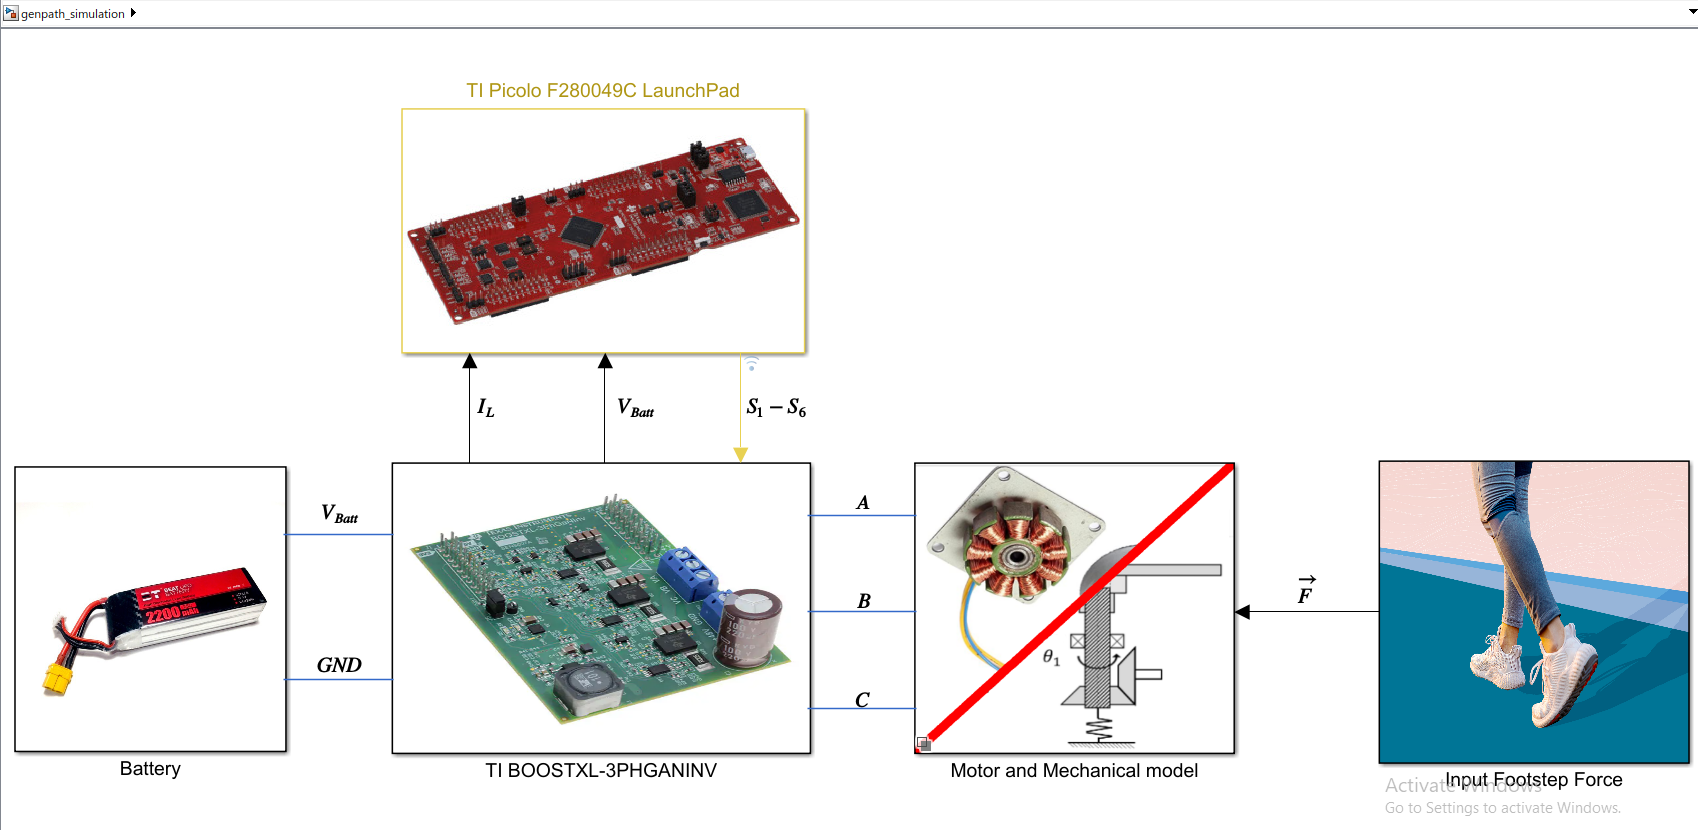
\includegraphics[width=\textwidth]{layer0.png}
    \caption{ภาพรวมของระบบแผ่นพื้นเก็บพลังงานที่ถูกสร้างในรายงานฉบับนี้}
\end{figure}

\subsection{ที่มาและความสำคัญของโครงงาน}
การเก็บเกี่ยวพลังงานจากการเคลื่อนไหวของมนุษย์นั้น เป็นเรื่องที่น่าสนใจ สามารถนำมาทำให้เกิดขึ้นจริงได้ เช่นในกรณีของแผ่นพื้นเก็บพลังงานนั้น ได้ถูกนำมาสร้างเป็นผลิตภัณฑ์ที่สามารถสร้างรายได้ และได้มีการติดตั้งใช้งานแล้วในหลายๆ ที่ เช่นกรณีตัวอย่างของ Pavegen\textsuperscript{TM} Pavegen\textsuperscript{TM} เป็นบริษัท Startup ที่สร้างแผ่นพื้นเก็บพลังงาน เพื่อที่จะจ่ายพลังงานให้กับอุปกรณ์ขนาดเล็ก เช่น เซนเซอร์ต่างๆ ที่เชื่อมต่อกับระบบอินเทอร์เน็ตของสรรพสิ่ง (Internet of Things; IoT) หรืออุปกรณ์ส่องสว่างประเภทหลอด LED หรือกักเก็บพลังงานไว้ในแบตเตอร์รี

\begin{figure}
    \centering
    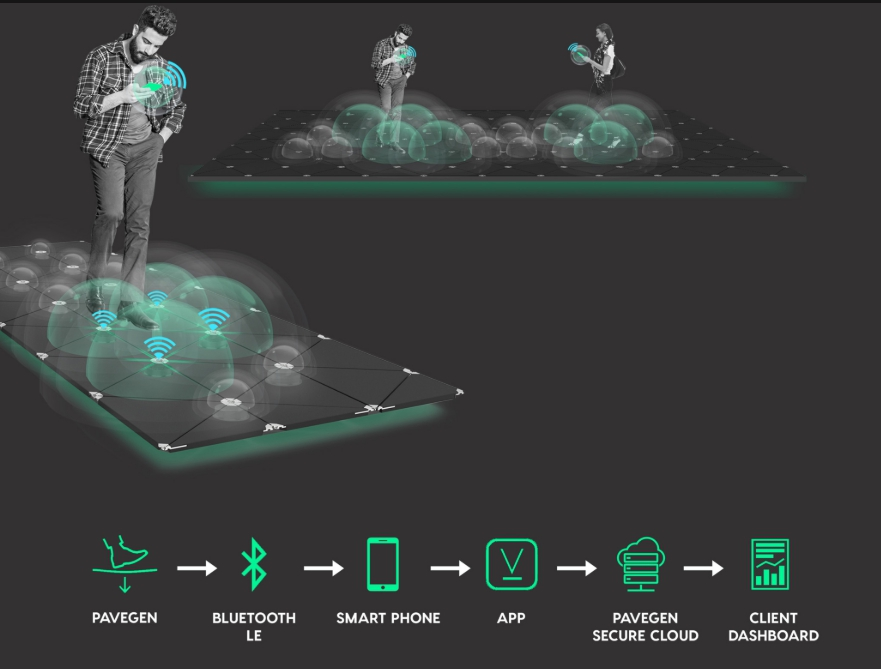
\includegraphics[width=\textwidth]{pavegen_poster.jpg}
    \caption{โปสเตอร์ของ Pavegen\textsuperscript{TM}}
\end{figure}

\begin{figure}
    \centering
    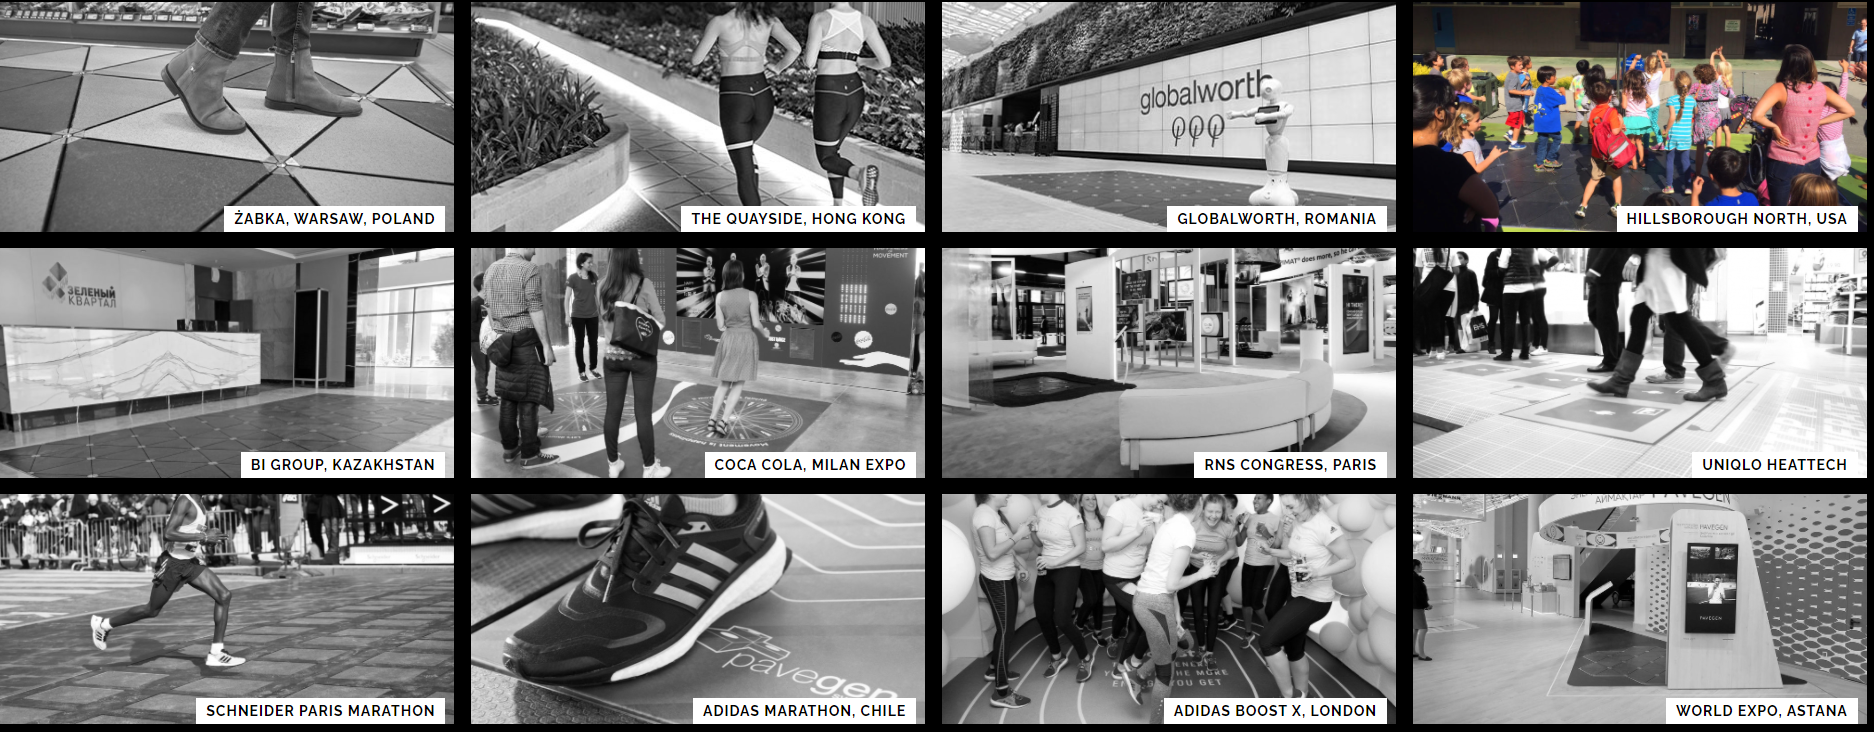
\includegraphics[width=\textwidth]{pavegen_usecase.png}
    \caption{สถานที่ที่ได้มีการติดตั้ง Pavegen\textsuperscript{TM}}
\end{figure}

จากค้นคว้าจากการศึกษาในครั้งก่อนๆ \cite{biomech} \cite{GpH:01} ได้ค้นพบว่า พลังงานที่ได้ในแต่ละการเหยียบแต่ละครั้งนั้น มีค่าน้อยมาก นั่นคือประมาณ 1-5 จูล เท่านั้น ดังนั้น หัวใจในการเก็บเกี่ยวพลังงานจากระบบดังกล่าว คือการมีประสิทธิภาพที่ดี จึงจะสามารถเก็บพลังงานได้เพียงพอกับการใช้งานต่อไป ดังนั้น การศึกษาในโครงงานฉบับนี้ จึงได้มุ่งเน้นในการเพิ่มประสิทธิภาพให้กับระบบเก็บพลังงานเป็นหลัก

จากโครงงานปี 2563 กำลังไฟฟ้าขาออกของเครื่องกำเนิดไฟฟ้าไม่ได้เป็นค่าสูงสุด โดยจากการทดสอบมีค่าประมาณ หนึ่งในสี่ ของพลังงานขาเข้าที่มาจากแรงเท้าเหยียบของมนุษย์ และไม่ได้มีการลดการกำลังสูญเสียของวงจรแปลงผัน โครงงานปี 2564 นี้ มีการพัฒนาการออกแบบทางไฟฟ้าและทางกลเพื่อประปรุงประสิทธิภาพของแผ่นพื้นเก็บพลังงาน โดยมี 2 ส่วน คือ

1.สร้างแบบจำลองทางไฟฟ้าที่รวมระบบทางกลของแผ่นพื้นเก็บพลังงานและเครื่องจักรไฟฟ้าซิงโครนัสชนิดแม่เหล็กถาวร เพื่อทราบเงื่อนไขของแรงดันออกตามหลักการติดตามจุดทำงานสูงสุด

2.การลดกำลังสูญเสียในอินเวอร์เตอร์ ด้วยอัลกอรึทึมการมอดูเลตแบบสองแขน และการติดตามการทำงานในจตุภาคที่หนึ่ง


\subsection{วัตถุประสงค์ของโครงงาน}
\begin{enumerate}
    \item เพื่อศึกษาแบบจำลองทางคณิตศาสตร์และสร้างแบบจำลองพลวัตของระบบแผ่นพื้นเก็บพลังงานด้วยโปรแกรม MATLAB\textsuperscript{TM}/Simulink\textsuperscript{TM} เพื่อตรวจสอบผลลัพธ์ที่ได้ก่อนนำไปใช้กับอุปกรณ์จริง
    \item เพื่อหาแนวทางในการลดพลังงานสูญเสียในระบบขับเคลื่อนเครื่องจักรกลไฟฟ้าซิงโครนัสประเภทแม่เหล็กถาวร และพัฒนาชุดอัลกอริทึมในการเพิ่มประสิทธิภาพให้กับระบบแผ่นพื้นเก็บพลังงาน
    \item เพื่อสร้างต้นแบบอุปกรณ์ แผ่นพื้นเก็บพลังงาน ที่สามารถใช้งานได้จริง

\end{enumerate}

\subsection{ขอบเขตของโครงงาน}
\begin{enumerate}
    \item โครงงานฉบับนี้จะใช้เครื่องจักรกลไฟฟ้าชนิดแม่เหล็กถาวร เป็นตัวกำเนิดไฟฟ้า
    \item โครงงานฉบับนี้จะใช้ไมโครคอนโทรลเลอร์ TI\textsuperscript{TM} F280049C ที่อยู่บนชุดทดลอง Picolo\textsuperscript{TM} LaunchPad\textsuperscript{TM} เป็นระบบฝังตัวแกนกลางในคำนวนอัลกอริทึมต่างๆ
    \item โครงงานฉบับนี้จะใช้บอร์ดอินเวอร์เตอร์ TI\textsuperscript{TM} BOOSTXL-3PHGaNINV เป็นสวิตช์สำหรับวงจรอินเวอร์เตอร์
    \item โครงงานฉบับนี้จะโปรแกรมระบบฝังตัวดังกล่าวผ่านการสร้างโค๊ดบนแพลตฟอร์ม Simulink\textsuperscript{TM} Embedded Coder\textsuperscript{TM}
\end{enumerate}

\subsection{ผลลัพธ์ที่คาดหวังจากโครงงาน}

\begin{enumerate}
    \item แผ่นพื้นเก็บพลังงานต้นแบบที่มีประสิทธิภาพสูง และสามารถใช้งานได้จริง
    \item อัลกอริทึมในการลดกำลังสูญเสียในอินเวอร์เตอร์ ที่สามารถนำไปใช้กับระบบแผ่นพื้นเก็บพลังงาน และยังสามารถนำไปใช้กับอินเวอร์เตอร์ใดๆ นอกเหนือจากระบบแผ่นพื้นเก็บพลังงานได้อีกด้วย
    \item อัลกอริทึมในการติดตามจุดทำงาน ที่ให้กำลังไฟฟ้าสูงสุด ที่สามารถนำไปใช้กับระบบแผ่นพื้นเก็บพลังงาน
\end{enumerate}

\section{หลักการและทฤษฎีที่เกี่ยวข้อง}

\subsection{การลดกำลังสูญเสียในอินเวอร์เตอร์ ด้วยอัลกอริทึมการมอดูเลตแบบสองแขน และการติดตามการทำงานในจตุภาคที่หนึ่ง (Two Arm Modulation and First Quadrant Tracking Algorithm)}

\subsubsection{การมอดูเลตความกว้างพัลส์แบบใช้สัญญาณพาหะ และ อินเวอร์เตอร์โหมดแรงดันแบบสามเฟส}
ในการขับเคลื่อนเครื่องจักรกลไฟฟ้าโดยทั่วไปนั้นอาศัยการสร้างสนามแม่เหล็กหมุน มาเหนี่ยวนำให้เกิดแรงบิด ซึ่งในกรณีของเครื่องจักรกลไฟฟ้าซิงโครนัสแบบแม่เหล็กถาวรนั้นอาศัยการสร้างสนามแม่เหล็กหมุนโดยใช้ไฟฟ้ากระแสสลับ อินเวอร์เตอร์ จึงเป็นอุปกรณ์ที่จำเป็นต่อระบบขับเคลื่อนเครื่องจักรกลไฟฟ้าซิงโครนัสแบบแม่เหล็กถาวรด้วยแหล่งจ่ายไฟฟ้ากระแสตรง ในโครงงานฉบับนี้ ได้นำเครื่องจักรกลไฟฟ้าซิงโครนัสแบบแม่เหล็กถาวรสามเฟส มาเป็นเครื่องกำเนิดไฟฟ้า สำหรับระบบแผ่นพื้นเก็บพลังงาน โดยจะเก็บพลังงานที่ผลิตได้ไว้กับแบตเตอร์รี ในโครงงานฉบับนี้ จึงเลือกใช้อินเวอร์เตอร์สามเฟสที่มีทอพอโลยีดังรูปที่ \ref{3phaseinv}
\begin{figure}[!h]
    \centering
    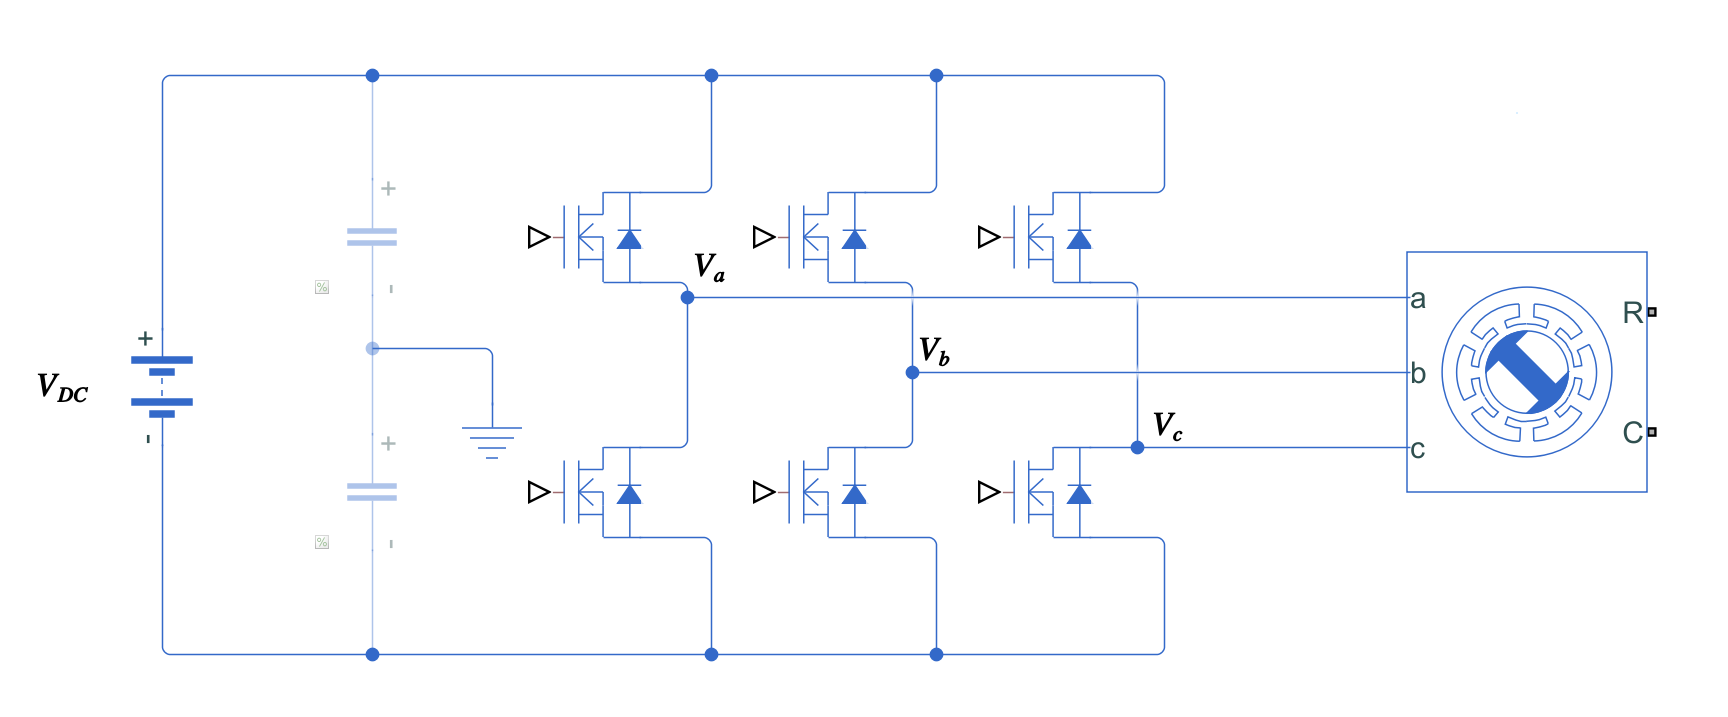
\includegraphics[width=\textwidth]{inverter_topology.png}
    \caption{ทอพอโลยีของอินเวอร์เตอร์สามเฟส}
    \label{3phaseinv}
\end{figure}

อินเวอร์เตอร์ทอพอโลยีที่ได้นำเสนอมาข้างต้น สามารถสร้างแรงดันออกที่แต่ละขั้วทั้งสามได้เพียงแค่ 2 ค่าเท่านั้นคือ
\begin{equation}
    V_t = \begin{cases}
        V_{DC}, & \text{ถ้าสวิตช์ตัวบนปิด และสวิตช์ตัวล่างเปิด} \\
        0,      & \text{ถ้าสวิตช์ตัวบนปิด และสวิตช์ตัวล่างเปิด}
    \end{cases}
\end{equation}
โดยที่ $V_t$ เป็นแรงดันที่ขั้วออกของอินเวอร์เตอร์
และถ้าหากพิจารณาให้กึ่งกลางบัสแรงดันไฟฟ้ากระแสตรงเป็นจุดอ้างอิงแรงดัน จะได้ว่า
\begin{equation}
    V_{t0} = \begin{cases}
        V_{DC}/2,  & \text{ถ้าสวิตช์ตัวบนปิด และสวิตช์ตัวล่างเปิด} \\
        -V_{DC}/2, & \text{ถ้าสวิตช์ตัวบนปิด และสวิตช์ตัวล่างเปิด}
    \end{cases}
\end{equation}

เนื่องจากกระขับเคลื่อนเครื่องจักรกลไฟฟ้าซิงโครนัสสามเฟสประเภทแม่เหล็กถาวรนั้น จำเป็นต้องใช้ไฟฟ้ากระแสสลับคลื่นรูปไซน์ ดังนั้น เทคนิคการมอดูเลตความกว้างพัลส์โดยใช้สัญญาณพาหะ (Carrier-based Pulse Width Modulation) จึงได้ถูกนำมาใช้ โดยการมอดูเลตความกว้างพัลส์โดยใช้สัญญาณพาหะมีหลักการในการทำงานคือ นำสัญญาณพาหะรูปสามเหลี่ยม มาเปรียบเทียบกับสัญญาณคำสั่ง โดยผลลัพธ์ของการเปรียบเทียบนั้น จะได้เป็นสัญญาณขับนำของสวิตช์ ดังรูปที่ \ref{cbpwm} ซึ่งจะส่งผลให้ แรงดันที่ขั้วของอินเวอร์เตอร์ มีค่าเฉลี่ยเท่ากับแรงดันคำสั่ง

\begin{figure}[!h]
    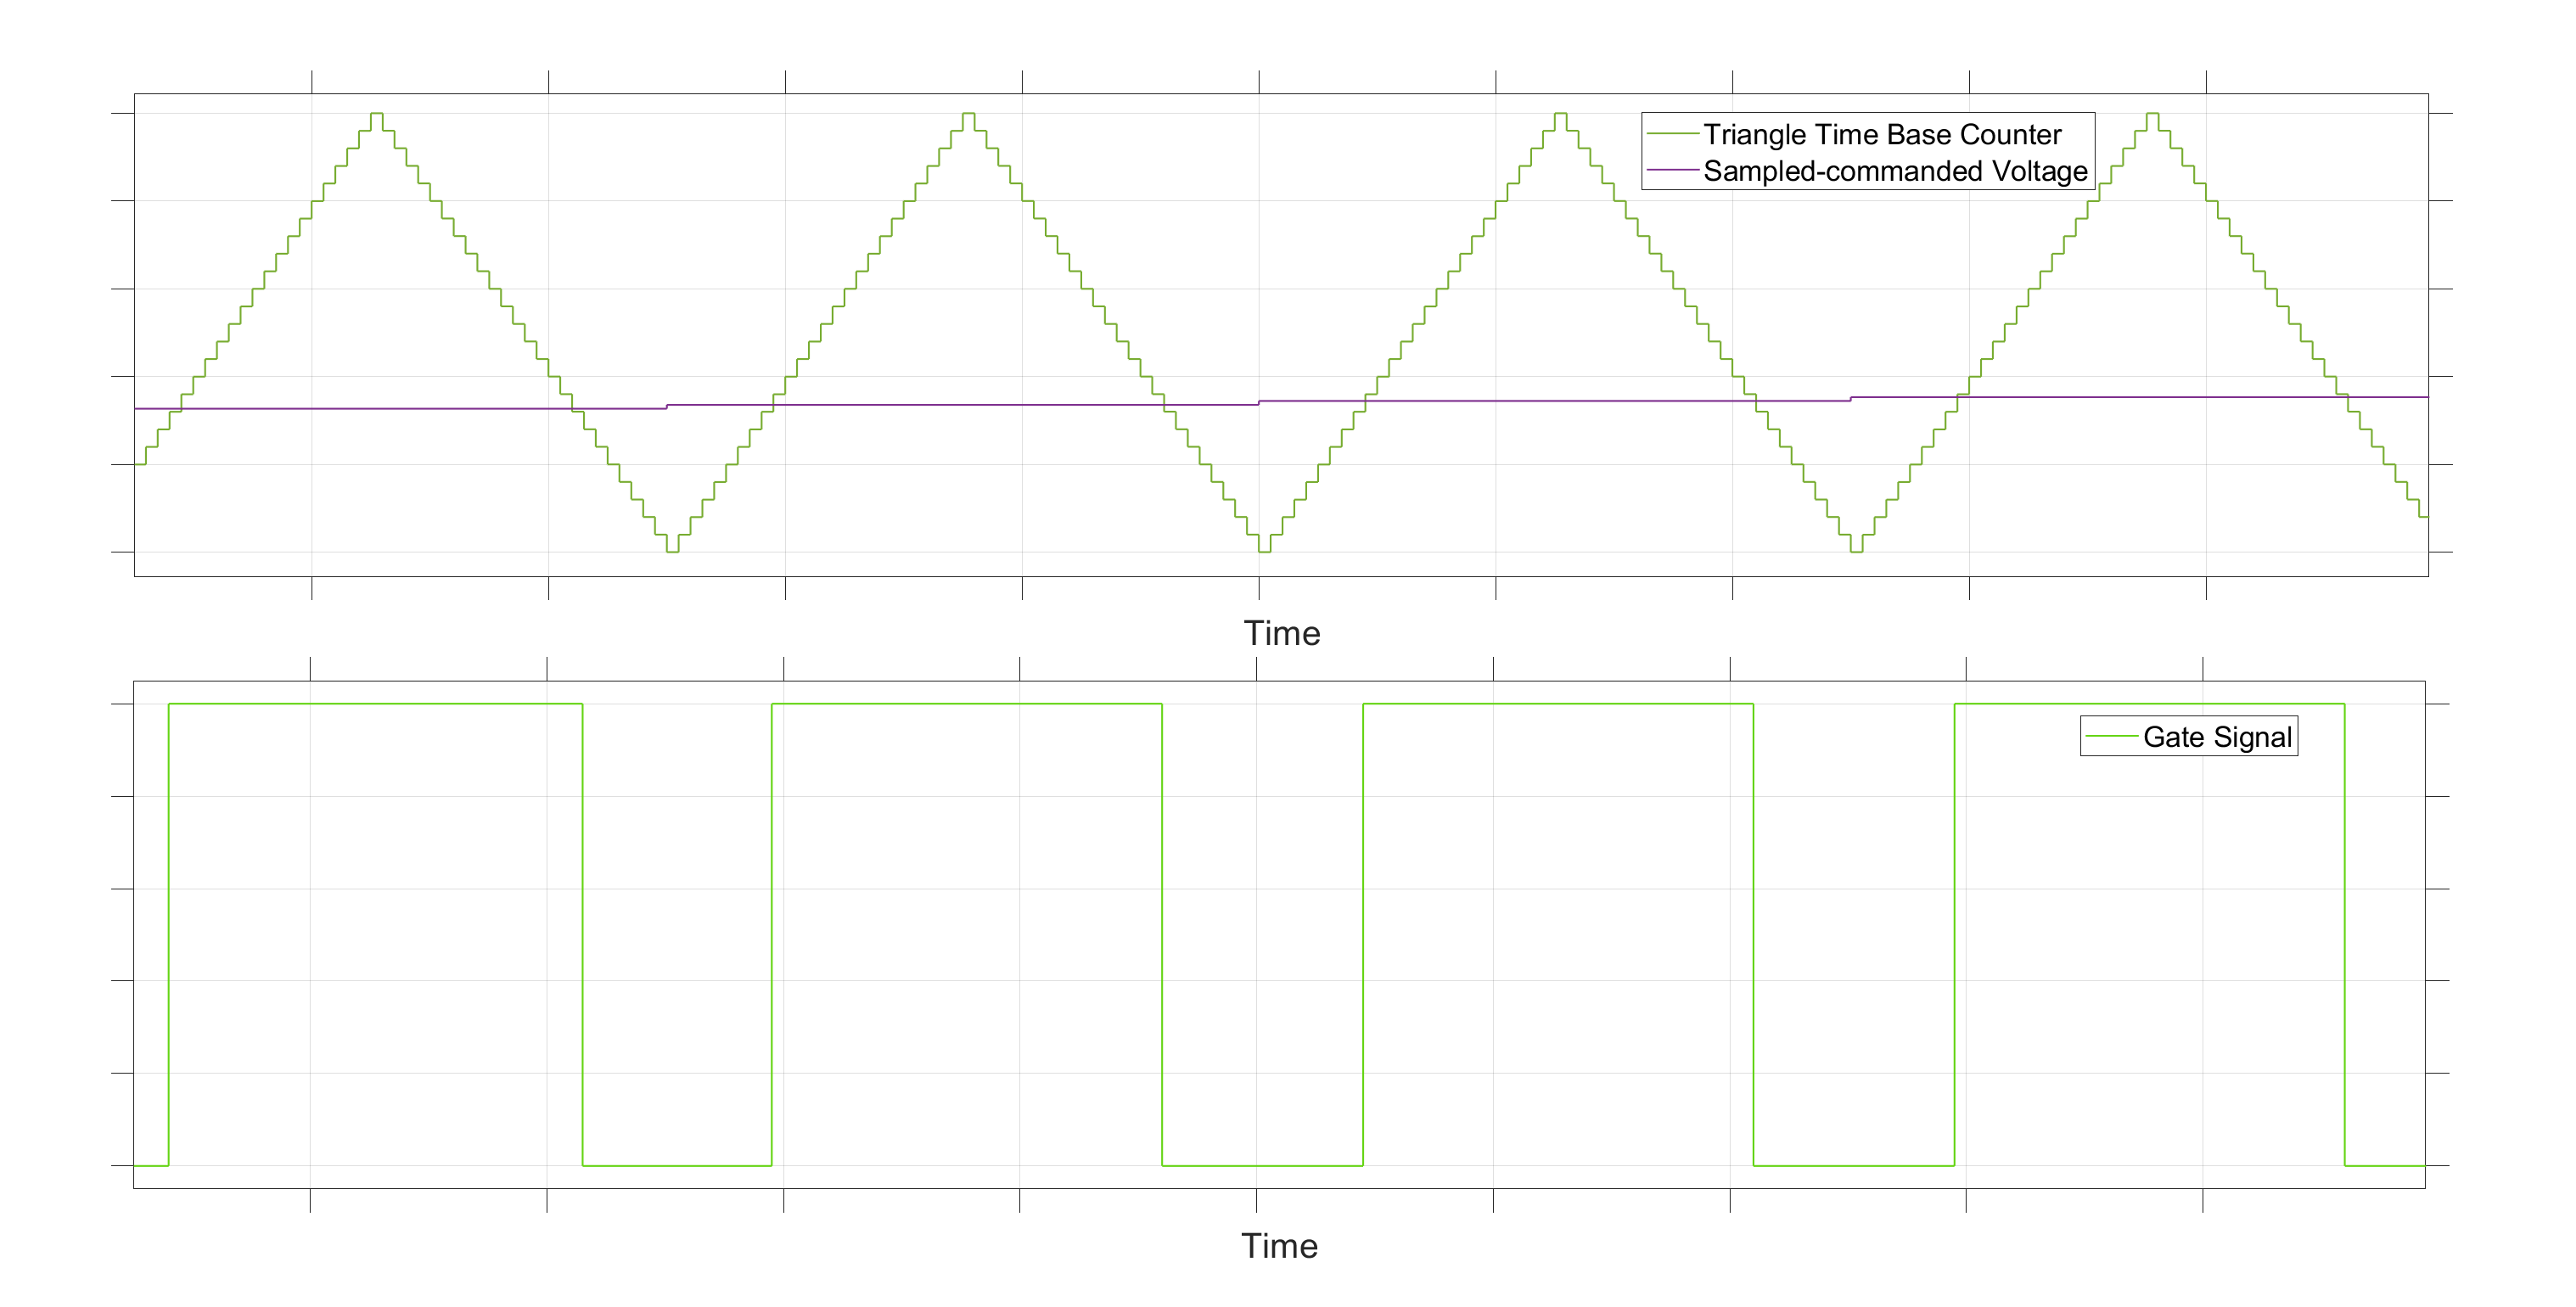
\includegraphics[width=\textwidth]{spwm.eps}
    \caption{การมอดูเลตความกว้างพัลส์โดยใช้สัญญาณพาหะ}
    \label{cbpwm}
\end{figure}

จากรูปข้างต้น จะเห็นได้ว่าความกว้างพัลส์ของสัญญาณขับนำนั้น เปลี่ยนไปตามขนาดของสัญญาณคำสั่ง และสัญญาณที่จะนำมาเปรียบเทียบนั้น จะเป็นสัญญาณที่ถูกสุ่มตัวอย่างแล้วคงค่า (Sample and Hold) เพราะว่า อัลกอริทึมการมอดูเลตที่เลือกใช้ในโครงงานฉบับนี้นั้น เป็นการคำนวนบนระบบฝังตัว ซึ่งเป็นการประมวลผลในโดเมนดิจิทัล

\subsubsection{กำลังสูญเสียในสวิตช์ของอินเวอร์เตอร์}
กำลังสูญเสียในสวิตช์ของอินเวอร์เตอร์มีอยู่ด้วยกันสองประเภท คือ กำลังสูญเสียระหว่างสวิตช์ (Switching Loss) และกำลังสูญเสียระหว่างนำกระแส (Conduction Loss)
\begin{equation}
    P_{loss} = P_{sw} + P_{cond}
\end{equation}

\begin{figure}[h]
    \centering
    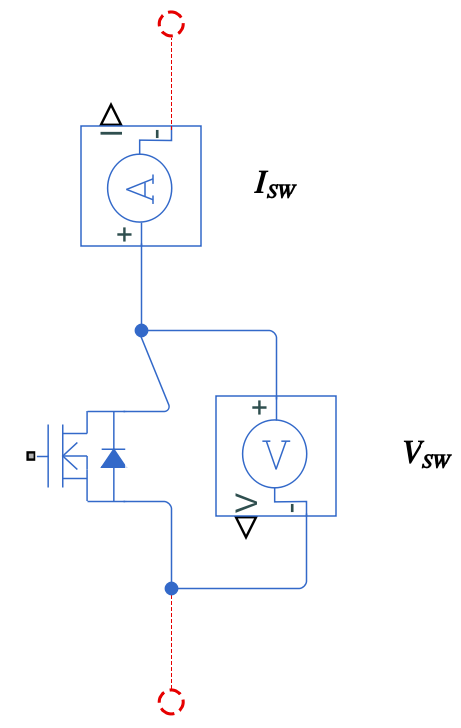
\includegraphics[width=0.25\textwidth]{vsw_isw.png}
    \caption{นิยามของ $V_{SW}, I_{SW}$}
    \label{vsw_isw_definition}
\end{figure}

\begin{figure}[h!]
    \centering
    \begin{tikzpicture}
        \pgfplotsset{width=\textwidth,height=\textwidth/3}
        \begin{axis}[
                axis x line=middle,
                axis y line=middle,
                xlabel=$Time$,
                xmax=45,
                ymax=25,
                ytick=\empty,
                xtick=\empty,
                xlabel near ticks,
                xmin=0,
                ymin=0,
                every axis plot/.append style={ultra thick}
            ]
            % Plots
            \draw[fill=pink,opacity=0.2] (axis cs:2,0) rectangle (axis cs:10,25);
            \node at (axis cs:6,22) {\tiny $Switch-On$ $Region$};
            \draw[fill=green,opacity=0.2] (axis cs:10,0) rectangle (axis cs:25,25);
            \node at (axis cs:18,22) {\tiny $Conduction$ $Region$};
            \draw[fill=pink,opacity=0.2] (axis cs:25,0) rectangle (axis cs:32,25);
            \node at (axis cs:29,22) {\tiny $Switch-Off$ $Region$};
            \addplot[color=red] coordinates {(0,20) (5,20) (10,1) (25,1) (30,20) (35,20)};
            \addplot[color=blue] coordinates {(0,0) (2,0) (8,15) (27,15) (32,0) (35,0)};
            \legend{\tiny $V_{SW}$,\tiny $I_{SW}$}
        \end{axis}
    \end{tikzpicture}
    \begin{tikzpicture}
        \pgfplotsset{width=\textwidth,height=\textwidth/3}
        \begin{axis}[
                axis x line=middle,
                axis y line=middle,
                xlabel=$Time$,
                xmax=45,
                ymax=25,
                ytick=\empty,
                xtick=\empty,
                xlabel near ticks,
                xmin=0,
                ymin=0,
                every axis plot/.append style={ultra thick}
            ]
            % Plots
            \draw[fill=pink,opacity=0.2] (axis cs:2,0) rectangle (axis cs:10,25);
            \node at (axis cs:6,22) {\tiny $Switch-On$ $Region$};
            \draw[fill=green,opacity=0.2] (axis cs:10,0) rectangle (axis cs:25,25);
            \node at (axis cs:18,22) {\tiny $Conduction$ $Region$};
            \draw[fill=pink,opacity=0.2] (axis cs:25,0) rectangle (axis cs:32,25);
            \node at (axis cs:29,22) {\tiny $Switch-Off$ $Region$};
            \addplot[color=orange] coordinates {(5,0) (7.77,10) (8,8) (10,2) (25,2) (27,8) (27.33,10) (32,0)};
            \legend{\tiny $P_{loss}$}
        \end{axis}
    \end{tikzpicture}

    \caption{แรงดันตกคร่อมสวิตช์ กระแสของสวิตช์ และกำลังสูญเสียในสวิตช์}
    \label{switchloss}
\end{figure}

จากรูปที่ \ref{switchloss} จะเห็นได้ว่า ในขณะที่กำลังเปิดสวิตช์ กระแสและแรงดันตกคร่อมสวิตช์จะเหลื่อมกัน ซึ่งเกิดจากโครงสร้างทางกายภาพของทรานซิสเตอร์ จะทำให้เกิดกำลังสูญเสียในขณะสวิตช์ ซึ่งจะคำนวณได้จาก

\begin{equation}
    P_{sw} = \frac{1}{T_{sw}}\int\limits_{T_{sw}}{v_{sw}(t)i_{sw}(t)dt}\; \text{เมื่อ $T_{sw}$ คือเวลาที่สวิตช์อยู่ในช่วงกำลังสวิตช์}
\end{equation}

แต่เมื่อพอสวิตช์เปิดเต็มที่แล้ว สวิตช์จะมีแรงดันตกคร่อมอยู่เล็กน้อย ทำให้เกิดกำลังสูญเสียในขณะนำกระแส
\begin{equation}
    P_{cond} = v_{sw(on)}i_{sw(on)}
\end{equation}
เมื่อ $v_{sw(on)},i_{sw(on)}$ คือแรงดันตกคร่อมสวิตช์ และกระแสที่ไหลผ่านสวิตช์ในขณะนำกระแส ตามลำดับ

กำลังสูญเสียระหว่างสวิตช์นั้น ขึ้นอยู่กับคุณลักษณะสมบัติของสวิตช์ที่เลือกใช้ และจำนวนครั้งในการสวิตช์ นั้นคือ ถ้าหากสวิตช์ที่เลือกใช้มีคุณลักษณะสมบัติที่ทำให้อยู่ในย่านกำลังสวิตช์นาน หรือมีจำนวนครั้งในการสวิตช์มาก ก็จะทำให้กำลังสูญเสียขณะสวิตช์สูงตามไปด้วย

กำลังสูญเสียขณะนำกระแสนั้น ขึ้นอยู่กับว่าในขณะนำกระแสนั้นมีแรงดันตกคร่อมสวิตช์มากแค่ไหน ถ้าหากแรงดันตกคร่อมสวิตช์มาก ก็จะทำให้กำลังสูญเสียขณะนำกระแสมากขึ้นตามมา

\subsubsection{การนำกระแสในจตุภาคที่ 3 ของทรานซิสเตอร์สนามไฟฟ้าแกลเลียม ไนไตรท์}
ทรานซิสเตอร์สนามไฟฟ้าแกลเลียม ไนไตรท์ หรือ แกน (Gallium Nitride; GaN) ถือเป็นทางเลือกที่ดีสำหรับผู้ออกแบบในงานอิเล็กทรอนิกส์กำลัง เพราะว่าทรานซิสเตอร์แกน มีข้อดีกว่าทรานซิสเตอร์แบบซิลิคอนในหลายด้านคือ การไม่มีบอดีไดโอด ซึ่งทำให้ไม่มี reverse recovery loss ในบอดีไดโอด ข้อได้เปรียบนี้ทำให้ทรานซิสเตอร์แบบแกนมีการกำลังสูญเสียในขณะสวิตช์น้อยกว่าแบบดั้งเดิม ทำให้ทำงานได้ที่ความถี่สูงขึ้น ใช้ทรานซิสเตอร์ตัวเล็กลงได้ และความร้อนน้อยลง ซึ่งในโครงงานฉบับนี้ ได้เลือกใช้ทรานซิสเตอร์แกนเป็นสวิตช์ในอินเวอร์เตอร์

เนื่องจากโครงสร้างที่ไม่เหมือนกันของทรานซิสเตอร์แบบแกน ทำให้การนำกระแสในจตุภาคที่สามของทรานซิสเตอร์แบบแกนนั้นแตกต่างไปจากทรานซิสเตอร์แบบซิลิคอน \cite{ganfet} คือ การนำกระแสผ่านบอดีไดโอด

เงื่อนไขที่จะทำให้ทรานซิสเตอร์แกนนำกระแสในทิศทางไปข้างหน้า (Forward) และย้อนกลับ (Reverse) เป็นไปดังรูปที่ \ref{gan_on_condition} คือ

\begin{figure}[h!]
    \centering
    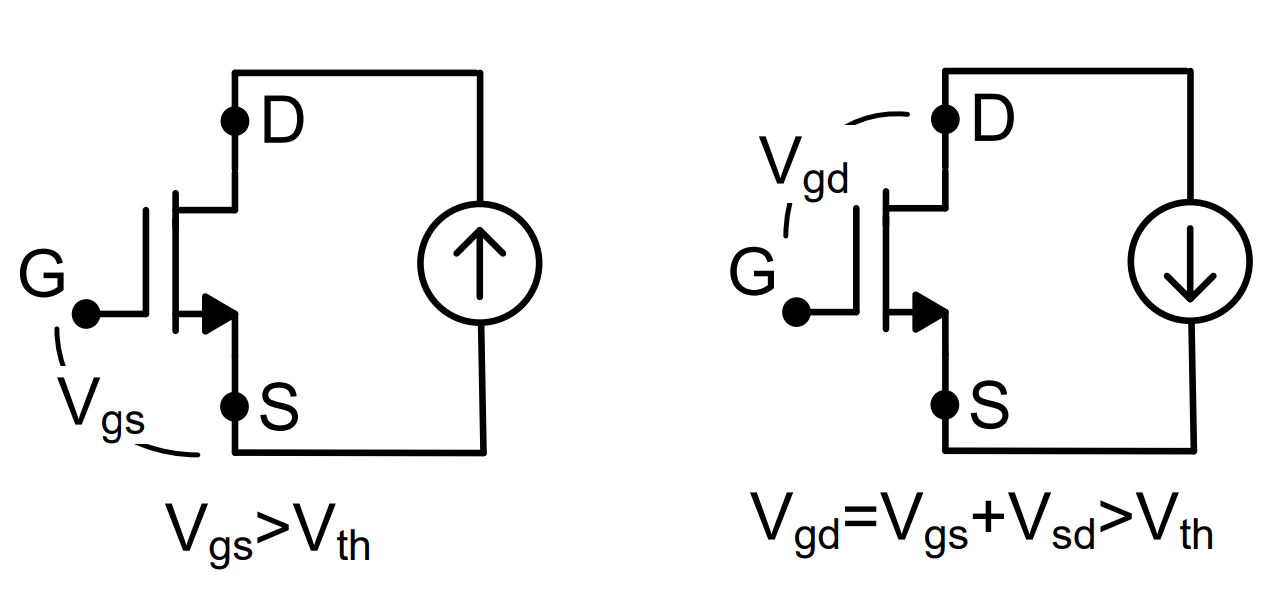
\includegraphics[width=0.4\textwidth]{gan_on_condition.png}
    \caption{เงื่อนไขที่จะทำให้ทรานซิสเตอร์แกนนำกระแสในทิศทางไปข้างหน้า และย้อนกลับ}
    \label{gan_on_condition}
\end{figure}

ถ้าหากพิจารณาตัวอย่างที่เกิดขึ้นจริงในอินเวอร์เตอร์เพื่อให้เห็นภาพพจน์ชัดเจนขึ้น ตามรูปวงจรของอินเวอร์เตอร์ ที่ตัดมาพิจารณาเฉพาะหนึ่งเฟส ตามรูปที่ \ref{inverter1p}

\begin{figure}[h!]
    \centering
    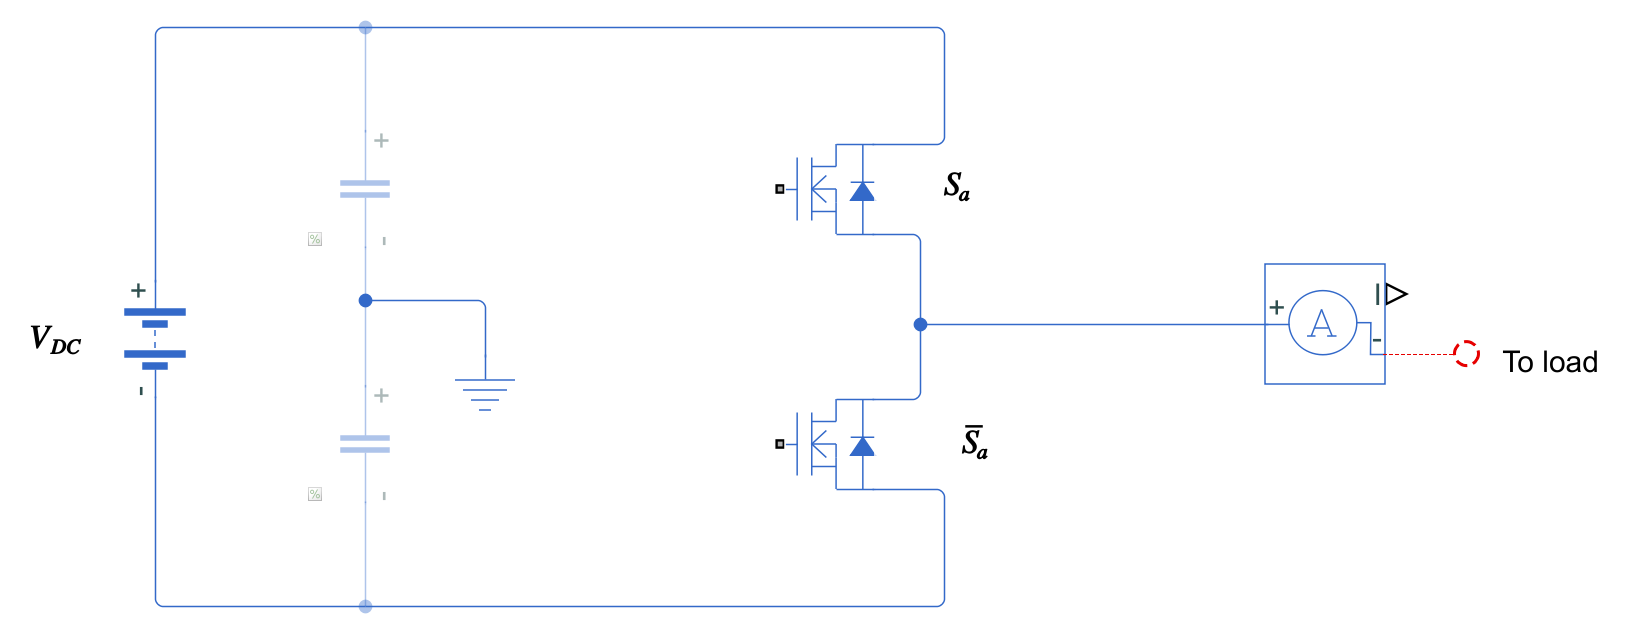
\includegraphics[width=0.7\textwidth]{first_third_inverter.png}
    \caption{กรณีตัวอย่างการนำกระแสที่เกิดขึ้นจริงในอินเวอร์เตอร์}
    \label{inverter1p}
\end{figure}

เรากำหนดให้สวิตช์ $S_a$ เป็นสวิตช์ที่เราสนใจ โดยถ้าหากเราขับนำสวิตช์ให้สวิตช์นำกระแส (On) นั่นคือ เราขับนำสัญญาณขา $V_{gs} > V_{th}$ แล้วถ้าหากโหลดที่ต่ออยู่กับขาซอร์สของสวิตช์ $S_a$ ดึงกระแสออกไปจากอินเวอร์เตอร์ นั่นคือ $I_a > 0$ จะทำให้ แรงดันตกคร่อมขาเดรนซอร์สของสวิตช์ $S_a$ เป็นค่าบวก นั่นคือ $V_{ds} > 0$ เนื่องจากสวิตช์ $S_a$ กำลังนำกระแสอยู่ ดังนั้นสวิตช์ $\bar{S_a}$ ไม่สามารถนำกระแสพร้อมๆ กับสวิตช์ $S_a$ ได้ เพราะจะลัดวงจร ดังนั้น กระแส $I_a$ ทั้งหมด ก็จะไหลผ่านสวิตช์ $S_a$ ทำให้กระแส $I_{ds} = I_a > 0$ เนื่องจากกระแส $I_{ds} > 0$ และ $V_{ds} > 0$ ดังนั้น สวิตช์จะนํากระแสในทิศทางไปข้างหน้า จุดทำงานที่กล่าวถึงข้างต้นจะแสดงในรูป \ref{inverter_q1}

\begin{figure}[h!]
    \centering
    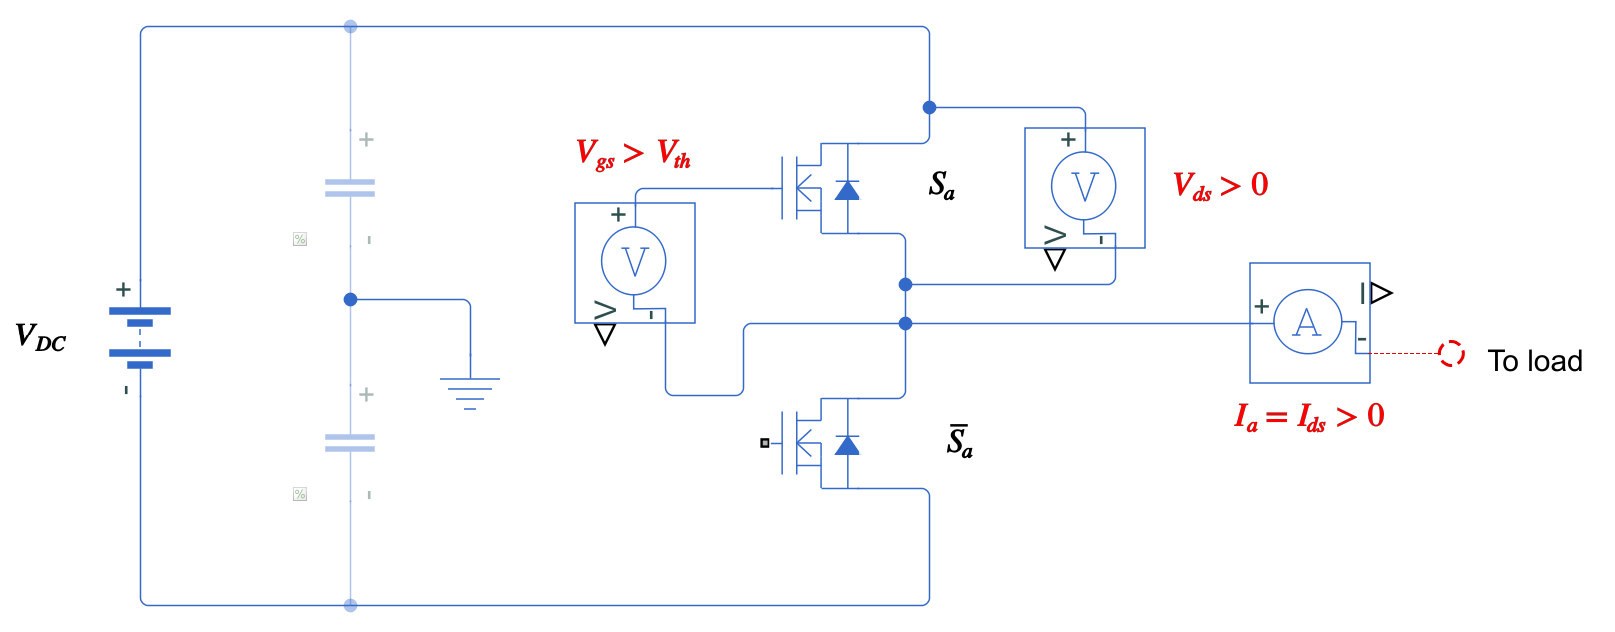
\includegraphics[width=0.7\textwidth]{inverter_q1.png}
    \caption{กรณีตัวอย่างการนำกระแสในทิศทางไปข้างหน้า: $V_{gs} > V_{th}$, $I_{ds} > 0$}
    \label{inverter_q1}
\end{figure}

ถ้าหากพิจารณากรณีถัดไปคือการขับนำสวิตช์ในลักษณะเดิมคือ การขับสัญญาณขา $V_{gs} > V_{th}$ แต่มีสิ่งที่เปลี่ยนไปคือ ทิศทางการไหลของกระแส นั่นคือ ถ้าหากโหลดมีการดึงกระแสเข้าอินเวอร์เตอร์ $I_a = I_{sd} >0$ จะทำให้ แรงดันตกคร่อมขาเดรนซอร์สของสวิตช์เป็นค่าลบ นั่นคือ $V_{ds} <0; V_{sd} > 0$ เนื่องจาก $V_{gd} = V_{gs} + V_{sd} =($ ค่าที่มากกว่า $V_{th})+$ ค่าที่เป็นบวก ดังนั้น $V_{gd} > V_{th}$ และ $I_{ds} < 0$ ทำให้สวิตช์นำกระแสย้อนกลับ

\begin{figure}[h!]
    \centering
    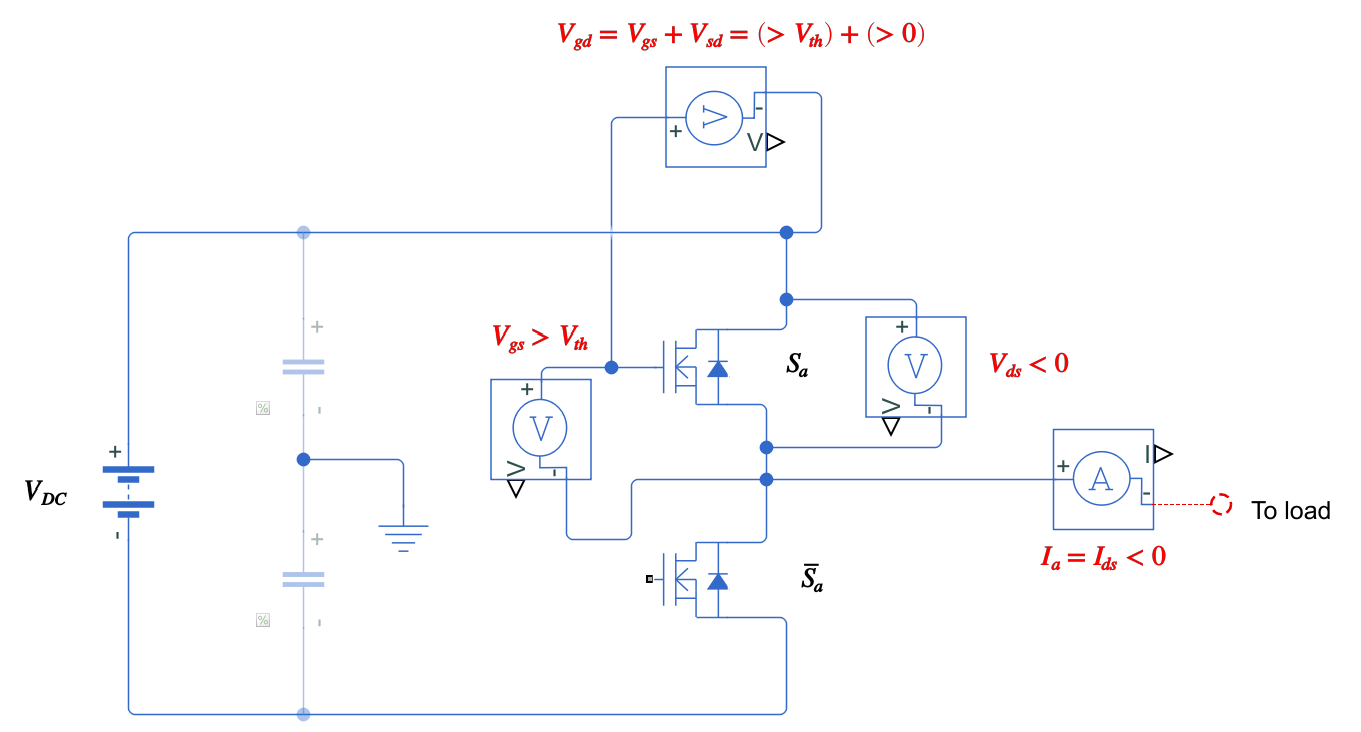
\includegraphics[width=0.7\textwidth]{inverter_q3.png}
    \caption{กรณีตัวอย่างการนำกระแสในทิศทางย้อนกลับ: $V_{gd} > V_{th}$, $I_{ds} < 0$}
    \label{inverter_q3}
\end{figure}

เราจะสามารถเขียนความสัมพันธ์ของกระแสและแรงดันขณะนำกระแสไปข้างหน้าได้โดย

\begin{equation}
    V_{ds} = I_{ds}R_{ds(on)}
\end{equation}

เมื่อแรงดันที่ขาเกตเทียบกับซอร์สของทรานซิสเตอร์ มากกว่าค่าแรงดันขีดแบ่ง และแรงดันที่ขาเดรนเทียบซอร์สเป็นบวก จะทำให้แกนนำกระแสในจตุภาคที่หนึ่ง โดยที่เรานิยาม $R_{ds(on)}$ เป็นความต้านทานสมมูลของทรานซิสเตอร์ในขณะที่กำลังทำงานในจตุภาคที่หนึ่ง

และเราก็สามารถเขียนคามสัมพันธ์ของกระแสและแรงดันขณะนำกระแสย้อนกลับได้โดย

\begin{equation}
    V_{sd} = I_{sd}R_{sd(on)}
\end{equation}

ในการนำกระแสย้อนกลับ ข้อมูลต่างๆ จะเป็นทวิลักษณ์ของข้อมูลในขณะนำกระแสไปข้างหน้าเลยคือ เมื่อแรงดันที่ขาเกตเทียบกับเดรน มากกว่าค่าแรงดันขีดแบ่ง และแรงดันที่ขาซอร์สเทียบกับเดรนเป็นบวก จะทำให้ทรานซิสเตอร์นำกระแสในจตุภาคที่สาม

\begin{figure}[h]
    \centering
    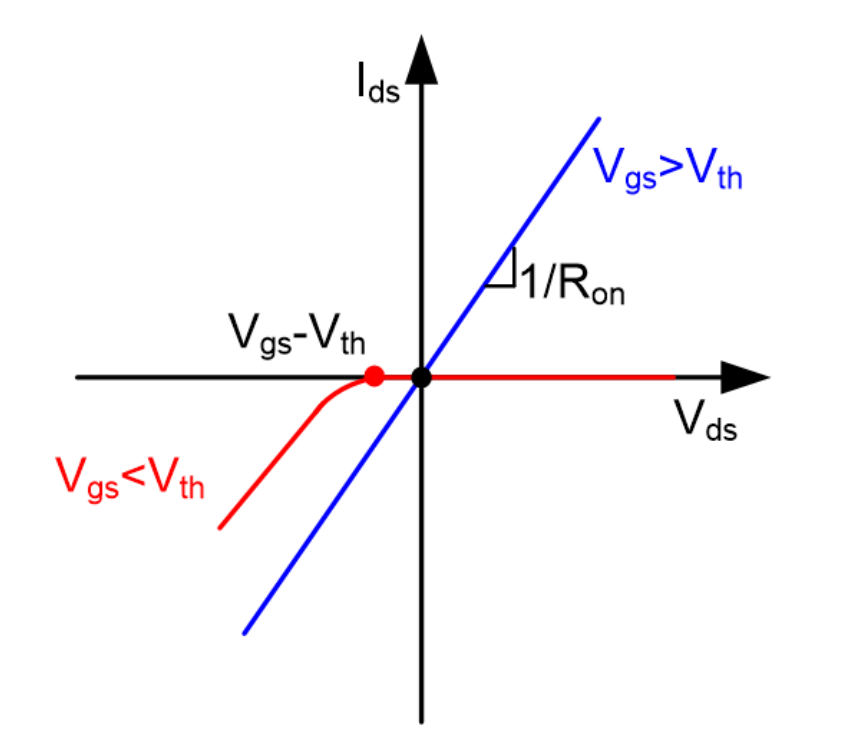
\includegraphics[width=0.4\textwidth]{gan_behavior.png}
    \caption{พฤติกรรมการนำกระแสในจตุภาคที่หนึ่ง และจตุภาคที่สามของทรานซิสเตอร์แกน}
    \label{gan_behavior}
\end{figure}

จากรูปที่ \ref{gan_behavior} จะเห็นได้ว่า แรงดันตกคร่อมทรานซิสเตอร์ในจตุภาคที่สาม จะมากกว่าแรงดันตกคร่อมทรานซิสเตอร์ในจตุภาคที่หนึ่งที่ค่ากระแสเท่ากัน ซึ่งทำให้การนำกระแสในจตุภาคที่สามนั้นมีกำลังสูญเสียในขณะนำกระแสมากกว่าการนำกระแสในจตุภาคที่หนึ่ง

\subsubsection{การลดกำลังสูญเสียในการมอดูเลตแบบใช้สัญญาณพาหะ ด้วยการมอดูเลตแบบสองแขน}

จากที่ได้นำเสนอไปแล้วในส่วนของการมอดูเลตแบบใช้สัญญาณพาหะ ว่า เป็นการมอดูเลตที่มีจำนวนครั้งในการสวิตช์มาก ซึ่งทำให้กำลังสูญเสียในขณะสวิตช์สูง แต่เรามีเทคนิคในการลดกำลังสูญเสียขขณะสวิตช์ในการมอดูเลตแบบใช้สัญญาณพาหะด้วยการลดจำนวนครั้งในการสวิตช์คือ การมอดูเลตแบบสองแขน

แขนของการมอดูเลต คือ คู่ของทรานซิสเตอร์ที่ใช้ในการสร้างแรงดันออกที่ขั้วของอินเวอร์เตอร์ จะประกอบไปด้วยทรานซิสเตอร์ตัวบน ซึ่งเป็นทรานซิสเตอร์ที่ต่ออยู่กับบัสแรงดันไฟตรงที่ขั้วบวก และทรานซิสเตอร์ตัวล่าง ซึ่งเป็นทรานซิสเตอร์ที่ต่ออยู่กับบัสแรงดันไฟตรงที่ขั้วลบ จากทอพอโลยีของอินเวอร์เตอร์ที่เราเลือกใช้ในโครงงานฉบับนี้ ซึ่งแสดงไว้ ณ รูปที่ \ref{3phaseinv} จะเห็นได้ว่า จะมีแขนของการมอดูเลตทั้งหมดสามแขน

จากการพิจารณาจะเห็นได้ว่า หากเราต้องการสร้างแรงดันรูปไซน์ที่ขั้วของอินเวอร์เตอร์ เราจำเป็นต้องสวิตช์ทั้งสามแขนไปพร้อมๆ กัน แต่ถ้าหากเราพิจารณาความจริงที่ว่า แรงดันที่สร้างกระแสของมอเตอร์ที่ต่อแบบสามเฟสสามสาย เป็นแรงดันระหว่างสาย คือ

\begin{eqnarray}
    v_{ab} &=& v_{a0} - v_{b0} \\
    v_{bc} &=& v_{b0} - v_{c0} \\
    v_{ca} &=& v_{c0} - v_{a0}
\end{eqnarray}

และถ้าหากเราเพิ่มแรงดันลำดับศูนย์ (Zero-sequence Offset) ให้กับแรงดันเฟสของอินเวอร์เตอร์

\begin{eqnarray}
    v_{a0}^* &=& v_{a0} + v_{N0} \\
    v_{b0}^* &=& v_{b0} + v_{N0} \\
    v_{c0}^* &=& v_{c0} + v_{N0}
\end{eqnarray}

แรงดันระหว่างสายของมอเตอร์จะมีค่าเท่าเดิม นั่นคือ

\begin{eqnarray}
    v_{ab}^* &=& v_{a0}^* - v_{b0}^* = v_{a0} + v_{N0} - (v_{b0} + v_{N0}) = v_{ab} \\
    v_{bc}^* &=& v_{b0}^* - v_{c0}^* = v_{b0} + v_{N0} - (v_{c0} + v_{N0}) = v_{bc} \\
    v_{ca}^* &=& v_{c0}^* - v_{a0}^* = v_{c0} + v_{N0} - (v_{a0} + v_{N0}) = v_{ca}
\end{eqnarray}

ดังนั้น เราสามารถเลือกแรงดันลำดับศูนย์ที่จะเพิ่มให้กับแรงดันเฟสคำสั่งของอินเวอร์เตอร์ โดยมีเป้าหมายคือ ทำให้แรงดันคำสั่งในเฟสใดเฟสหนึ่งของอินเวอร์เตอร์ มีค่าเท่ากับแรงดันบวก หรือลบของบัสแรงดันกระแสตรง เพื่อที่จะทำให้แขนของการมอดูเลตแขนนั้น ปิด หรือ เปิดตลอดเวลา นั่นคือ

\begin{equation}
    v_{N0} = \begin{cases}
        \frac{V_{DC}}{2}-max(v_{a0},v_{b0},v_{c0}); \text{ทรานซิสเตอร์ตัวบน on ตลอด} \\
        \frac{-V_{DC}}{2}-min(v_{a0},v_{b0},v_{c0}); \text{ทรานซิสเตอร์ตัวล่าง on ตลอด}
    \end{cases}
\end{equation}

ในขณะที่ทรานซิสเตอร์ตัวบนกำลังเปิดตลอดเวลา ทรานซิสเตอร์ตัวล่าง ก็จะปิดตลอดเวลาด้วย การให้ทรานซิสเตอร์แขนใดแขนหนึ่งเปิด หรือปิดตลอดเวลา จะทำให้ลดจำนวนครั้งในการสวิตช์ได้หนึ่งในสามเท่า ก็จะช่วยลดกำลังสูญเสียในขณะสวิตช์ได้

\subsubsection{การเพิ่มประสิทธิภาพให้กับการมอดูเลตแบบสองแขนด้วยการติดตามการทำงานในจตุภาคที่ 1}

จากผลลัพธ์ที่ได้อภิปรายมาในส่วนที่แล้ว เราได้ทราบว่า เรามีอิสระในเลือกการมอดูเลตสองแขนได้สองประเภทคือ แบบทรานซิสเตอร์ตัวบนนำกระแสตลอด และทรานซิสเตอร์ตัวล่างนำกระแสตลอด ดังนั้น เราจะใช้ข้อได้เปรียบนี้ ในการเลือกรูปแบบการมอดูเลตแบบสองแขนให้เกิดประสิทธิภาพสูงที่สุด นั่นคือ การหลีกเลี่ยงการทำงานในจตุภาคที่ 3 สำหรับทรานซิสเตอร์ตัวที่จะนำกระแสตลอดเวลา โดยจะมีหลักการในการคำนวนค่าแรงดันเฟสลำดับศูนย์ที่จะบวกเข้าไป เพื่อให้ได้ผลลัพธ์ตามที่ต้องการ ตามผังงานในรูปที่ \ref{twoarmflowchart} ซึ่งจากผังงานที่ได้นำเสนอไปข้างต้น เราสามารถนำไปสร้างเป็นแผนภาพการเปลี่ยนสถานะ บน Simulink\textsuperscript{TM}/Stateflow\textsuperscript{TM} ได้ดังที่แสดงไว้ในรูป

\begin{figure}[h!]
    \centering
    \begin{tikzpicture}[node distance=2cm]
        \node (start) [startstop] {เริ่มต้น};
        \node (cir1) [circle, below of = start,draw = black] {};
        \node (in1) [io,below of=cir1] {รับข้อมูลแรงดันคำสั่ง สุ่มตัวอย่างและคงค่ากระแสสาย};
        \node (pro1) [process,below of=in1] {คำนวนหาเฟสที่มีแรงดันเฟสคำสั่งมากที่สุด};
        \node (pro2) [process,right = 3cm of pro1] {คำนวนหาเฟสที่มีแรงดันเฟสคำสั่งน้อยที่สุด};
        \node (dec1) [decision,below = 1cm of pro1, text width = 2cm]
        {
            ถ้ามอดูเลตแบบ
            ทรานซิสเตอร์ตัวบน
            นำกระแสตลอดเวลา
            จะทำให้ทรานซิสเตอร์
            นำกระแสในจตุภาคที่หนึ่ง?
        };
        \node (dec2) [decision,below = 1cm of pro2,text width = 2cm]
        {
            ถ้ามอดูเลตแบบ
            ทรานซิสเตอร์ตัวล่าง
            นำกระแสตลอดเวลา
            จะทำให้ทรานซิสเตอร์
            นำกระแสในจตุภาคที่หนึ่ง?
        };
        \node (cir2) [circle, below = 1cm of dec1, draw=black] {};
        \node (cir4) [circle, below of = cir2, draw = black] {};
        \node (out1) [io,below = 1cm of cir4,text width = 1.5cm] {มอดูเลตสองแขนแบบทรานซิสเตอร์ตัวบนนำกระแสตลอดเวลา};
        \node (out2) [io,right = 1.5cm of out1,text width = 1.5cm] {มอดูเลตสองแขนแบบทรานซิสเตอร์ตัวล่างนำกระแสตลอดเวลา};
        \node (out3) [io,right = 1.5cm of out2,text width = 2cm] {แบ่งภาระงาน (Load Balancing) ระหว่างทรานซิสเตอร์ตัวบน และตัวล่าง};
        \node (cir3) [circle, below = 1cm of out1, draw = black] {};

        \draw [arrow] (start) -- (cir1);
        \draw [arrow] (cir1) -- (in1);
        \draw [arrow] (in1) -- (pro1);
        \draw [arrow] (in1) -| (pro2);
        \draw [arrow] (pro1) -- (dec1);
        \draw [arrow] (pro2) -- (dec2);
        \draw [arrow] (dec1) -- (cir2);
        \draw [arrow] (dec2) |- (cir2);
        \draw [arrow] (cir2) -- (cir4);
        \draw [arrow] (cir4) -- node[anchor = west] {(yes,no)} (out1);
        \draw [arrow] (cir4) -| node[anchor = north west] {(no,yes)} (out2);
        \draw [arrow] (cir4) -| node[anchor = north west] {else} (out3);
        \draw [arrow] (out1) -- (cir3);
        \draw [arrow] (out2) |- (cir3);
        \draw [arrow] (out3) |- (cir3);
        \draw [arrow] (cir3.west) -- +(-4.5cm,0) |- (cir1);
    \end{tikzpicture}

    \caption{ฝังงานของอัลกอริทึมในการคำนวณแรงดันลำดับศูนย์เพื่อติดตามการทำงานในจตุภาคที่หนึ่งของสวิตช์ที่ถูกมอดูเลตแบบสองแขน}
    \label{twoarmflowchart}
\end{figure}

\begin{figure}
    \centering
    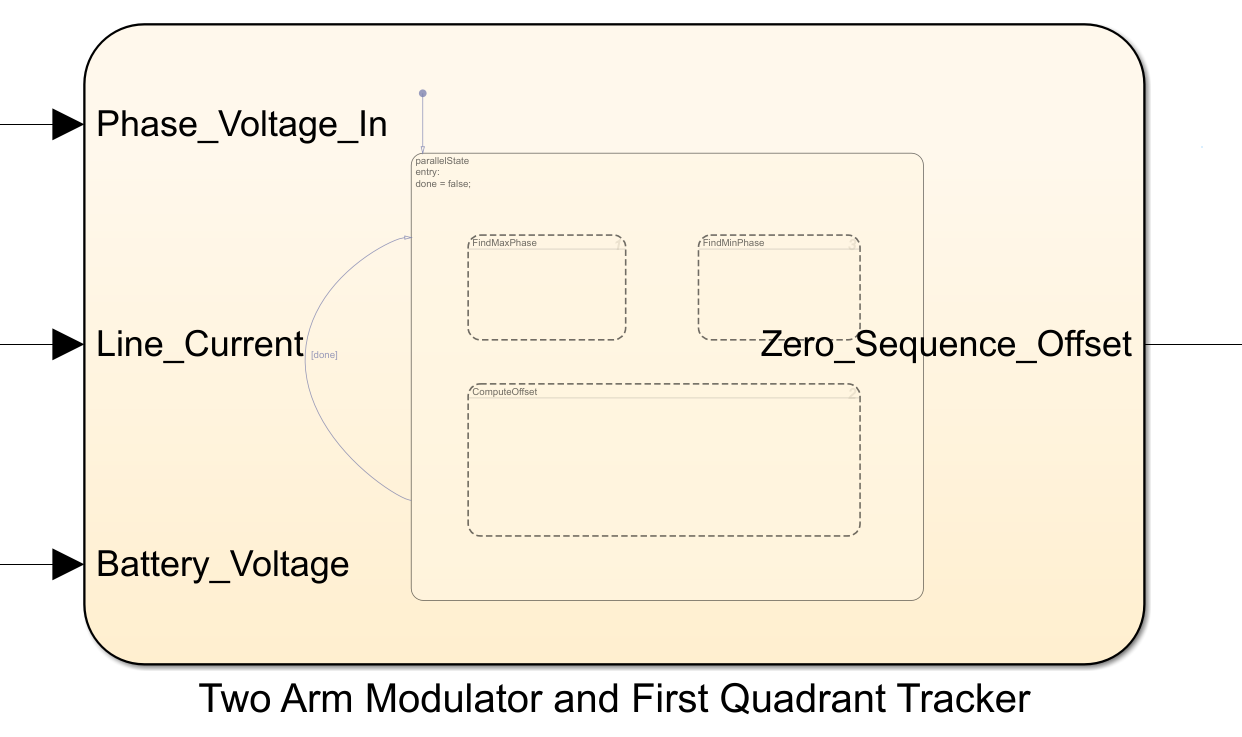
\includegraphics[width=0.4\textwidth]{tam-fqt-l0.png}
    \label{tam-fqt-l0}
    \caption{บล็อก Stateflow ของอัลกอริทึมในการมอดูเลตแบบสองแขน และการติดตามการทำงานในจตุภาคที่หนึ่ง}
\end{figure}

\begin{figure}
    \centering
    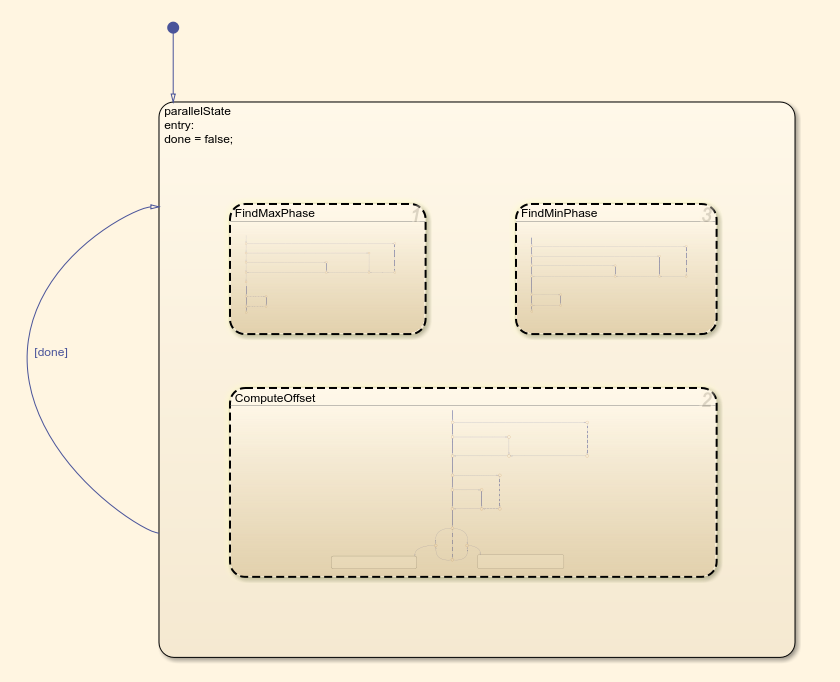
\includegraphics[width=0.8\textwidth]{tam-fqt-l1.png}
    \label{tam-fqt-l1}
    \caption{ภาพรวมของ Stateflow chart ของอัลกอริทึมในการมอดูเลตแบบสองแขน และการติดตามการทำงานในจตุภาคที่หนึ่ง}
\end{figure}

\begin{figure}
    \centering
    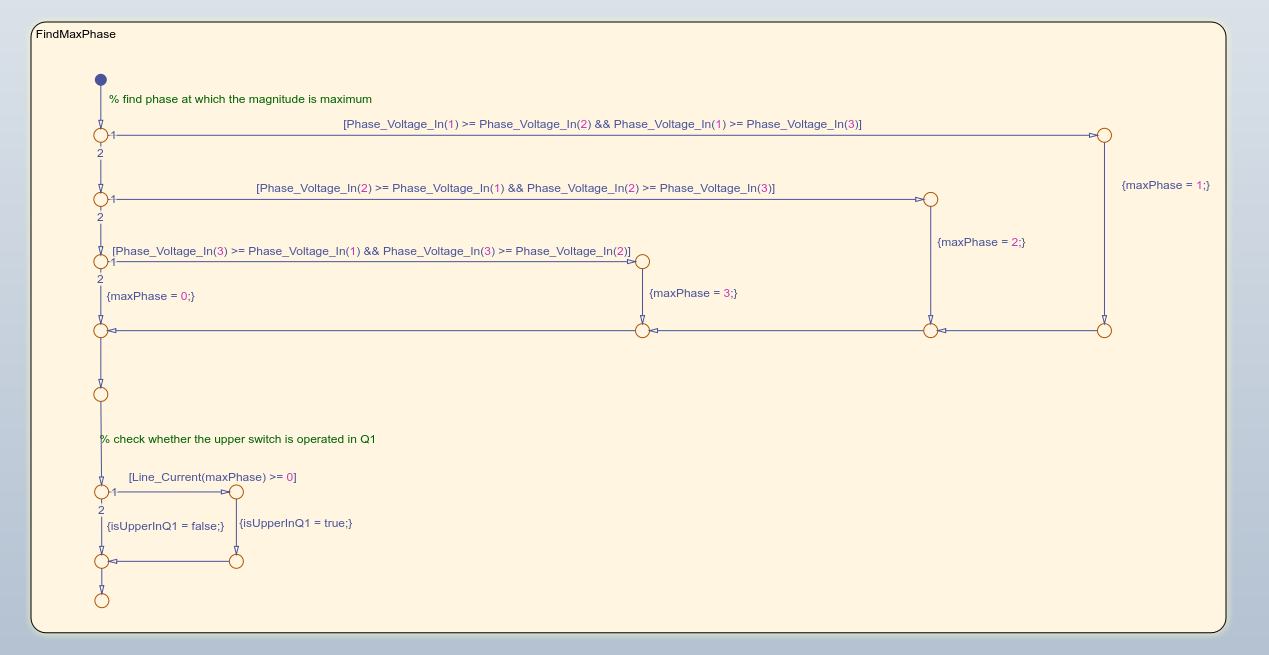
\includegraphics[width=\textwidth]{tam-fqt-l2-1.png}
    \label{tam-fqt-l2-1}
    \caption{Subchart ในส่วนของการหาเฟสที่มีแรงดันคำสั่งมากที่สุด}
\end{figure}

\begin{figure}
    \centering
    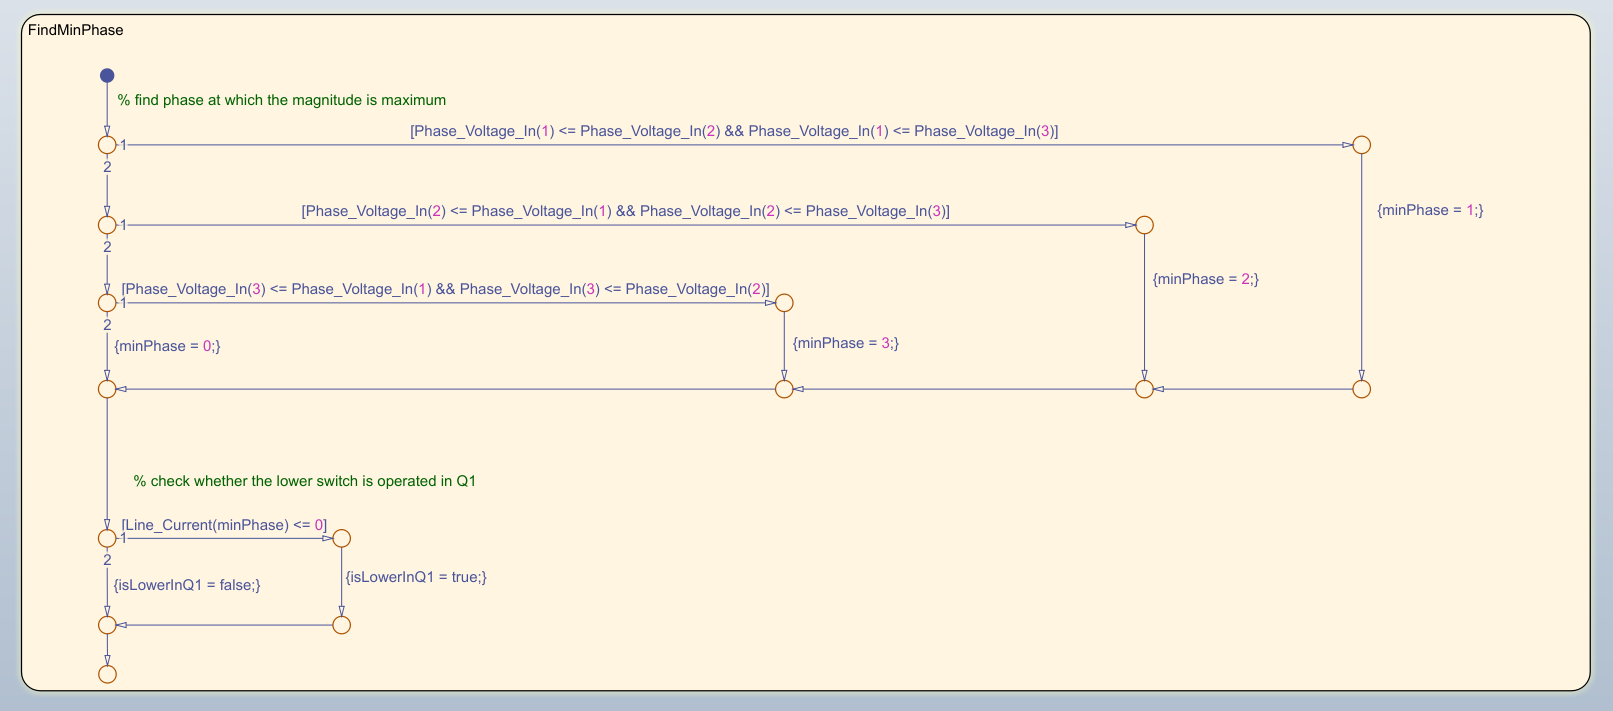
\includegraphics[width=\textwidth]{tam-fqt-l2-2.png}
    \label{tam-fqt-l2-2}
    \caption{Subchart ในส่วนของการหาเฟสที่มีแรงดันคำสั่งน้อยที่สุด}
\end{figure}

\begin{figure}
    \centering
    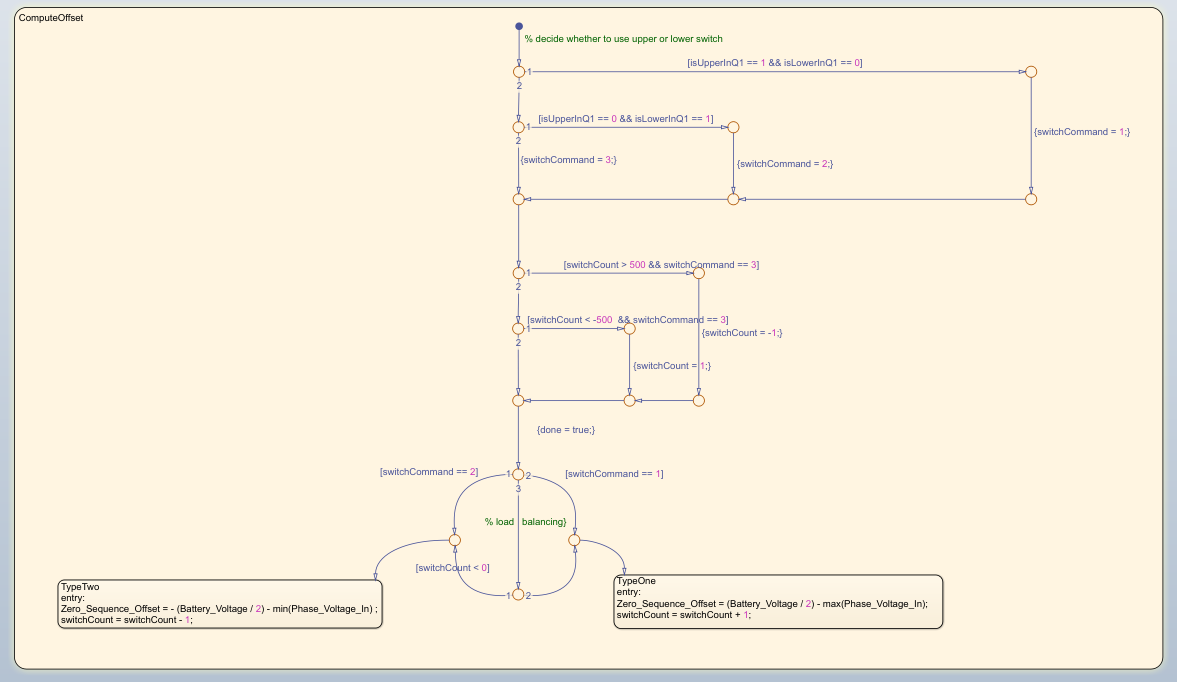
\includegraphics[width=\textwidth]{tam-fqt-l2-3.png}
    \label{tam-fqt-l2-3}
    \caption{Subchart ในส่วนของการคำนวนแรงดันลำดับศูนย์}
\end{figure}

\newpage
\subsection{การเพิ่มประสิทธิภาพของแผ่นพื้นเก็บพลังงานด้วยอัลกอริทึมการติดตามจุดทำงานที่ให้กำลังสูงสุด (Maximum Power Point Tracking Algorithm; MPPT)}
\subsubsection{ข้อมูลรายละเอียดและหลักการทำงานของแผ่นพื้นเก็บพลังงาน}
เริ่มแรกต้องศึกษาและเข้าใจหลักการทำงานของแผ่นพื้นเก็บพลังงานเพื่อทราบความสัมพันธ์ของกลไกและสมการต่างๆของระบบทางกลของแผ่นพื้นเก็บพลังงาน \cite{GpH:01}
และเข้าใจพลวัตของระบบทางกลของของแผ่นพื้นเก็บพลังงาน

แผ่นพื้นเก็บพลังงาน สามารถแปลงพลังงานจลน์จากการก้าวเดินของมนุษย์แปลงเป็นพลังงานไฟฟ้าจากเครื่องกำเนิดไฟฟ้าได้
หลักการทำงาน เริ่มจากการเหยียบของมนุษย์ลงบนแผ่นพื้นเก็บพลังงานทำให้เกิดการยุบตัวลงของแผ่นพื้น แป้นเกลียว(nut)จะขยับขึ้นลงไปขับเกลียวนำ(lead screw) ซึ่งทำหน้าที่เปลี่ยนแนวการเคลื่อนที่เชิงเส้นไปยังการเคลื่อนที่เชิงหมุน
ให้หมุนรอบแนวแกนตั้ง และ เฟืองดอกจอก(bevel gear)ทำหน้าที่เปลี่ยนจากเคลื่อนที่เชิงหมุนแนวแกนตั้งจากเพลาเกลียวนำให้เปลี่ยนทิศทางการหมุนไป 90 องศา หมุนรอบแนวนอน เพื่อขับเครื่องกำเนิดไฟฟ้า ดังรูปที่ \ref{lead-screw_lx}

\begin{figure}[h!]
    \begin{center}
        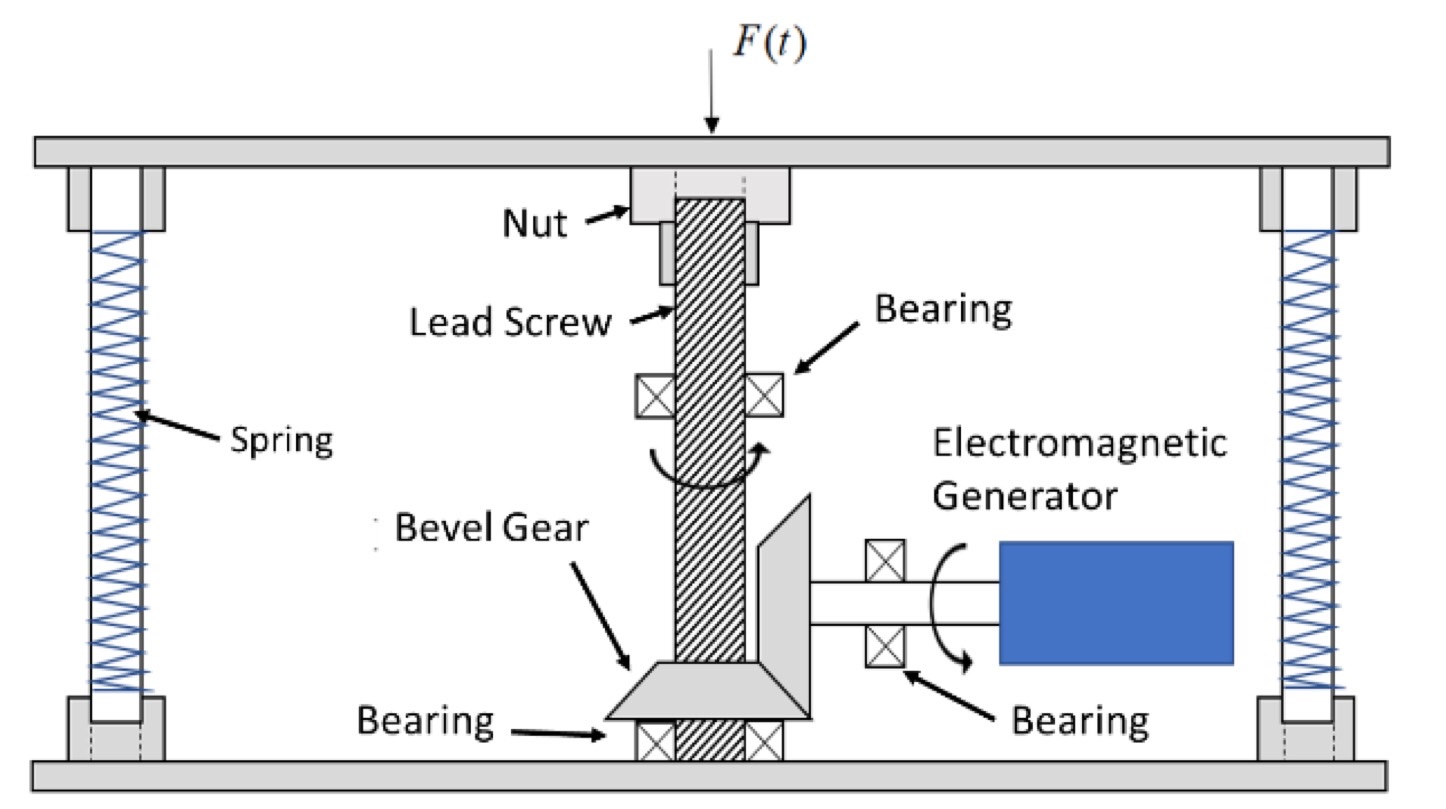
\includegraphics[width=0.5\textwidth]{lead-screw_lx.png}
    \end{center}
    \caption{กลไกเกลียวนำ(lead screw) ภายใต้แผ่นเก็บพลังงาน\cite{GpH:01}}
    \label{lead-screw_lx}
\end{figure}

จากแผนภาพของวัตถุของระบบทางกล ลีด(lead) และ สกรู(screw) ดังรูปที่ \ref{free_body_lx} สมการต่างๆ ได้มาจากกฎข้อที่สองของนิวตันและโมเมนตัมเชิงหมุน ซึ่งอธิบายการเลื่อนที่ของแป้นเกลียว และ การเคลื่อนที่เชิงหมุนของเกลียวนำและโรเตอร์ของเครื่องกำเนิดไฟฟ้า ตามลำดับ ได้แก่
\newpage
\begin{equation}
    m\ddot{x} = F(t)-F_{a}-F_{s}
\end{equation}

\begin{equation}
    J_{1}\ddot{\theta}_{1} = \frac{2\pi J_{1}}{l}\ddot{x} = T_{a}-T_{B}
\end{equation}

\begin{equation}
    J_{G}\ddot{\theta}_{2} = \frac{2\pi J_{G}}{l}\ddot{x} = T_{B}-T_{G}
\end{equation}

\begin{figure}[h!]
    \begin{center}
        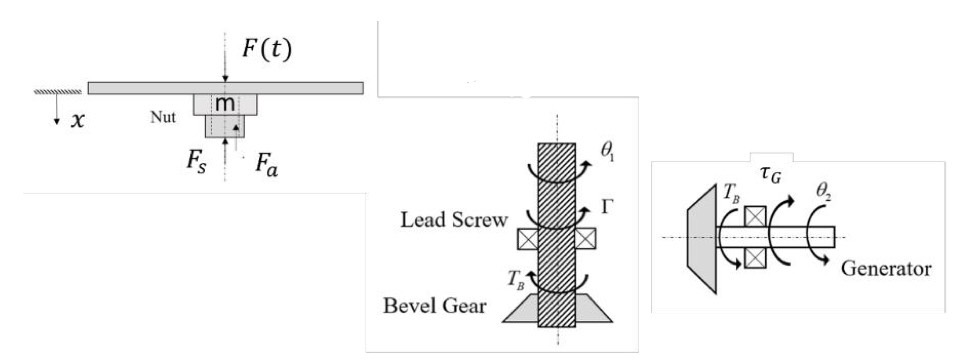
\includegraphics[width=0.7\textwidth]{free_body_lx.png}
    \end{center}
    \caption{แผนภาพของวัตถุของ lead screw}
    \label{free_body_lx}
\end{figure}

โดยที่

$m$ คือ มวลของแผ่นพื้นและแป้นเกลียว

$J_{1}$ คือ โมเมนต์ความเฉื่อยของเกลียวนำ

$J_{G}$ คือ โมเมนต์ความเฉื่อยของเฟืองดอกจอก

$x$ คือ ระยะกระจัดของแผ่นพื้นและแป้นเกลียว

$l$ คือ ระยะห่างระหว่างเกลียวของเกลียวนำ

$\theta_{1}$  คือ ตำแหน่งเชิงมุมของเกลียวนำ

$\theta_{2}$  คือ ตำแหน่งเชิงมุมของเฟืองดอกจอก

$F(t)$  คือ แรงกดลงบนแผ่นพื้นที่เวลาใดๆ

$F_{s}$   คือ แรงสปริง

$F_{a}$   คือ แรงเสียดทานระหว่างแป้นเกลียวและเกลียวนำ

$T_{B}$   คือ แรงบิดเสียดทานระหว่างแป้นเกลียวและเกลียวนำ

$T_{G}$   คือ แรงบิดแม่เหล็กไฟฟ้า (Electromagnetic torque)

$T_{a}$   คือ แรงบิดส่งผ่านจากแป้นเกลียว ไปยัง เกลียวนำ ซึ่งเป็นสัดส่วนโดยตรงกับ $F_{a}$ ดังนี้

\begin{equation}
    T_{a} = aF_{a}
\end{equation}

ค่าคงที่ a = $\frac{l}{2\pi \eta_{tread} \eta_{thrust}}$ เมื่อ $\eta_{tread}$ คือ ประสิทธิภาพของตลับลูกปืนคลัตซ์ และ $\eta_{trhust}$ คือ ประสิทธิภาพของเกลียว

\subsubsection{การเปรียบเทียบเชิงกล-ไฟฟ้า (Electrical analogy)}
ศึกษาหลักการการเปรียบเทียบเชิงกล-ไฟฟ้า(electrical analogy) \cite{ElecDrive} เพื่อเข้าใจความสัมพันธ์ของปริมาณทางกลและทางไฟฟ้า จากนั้นจึงนำไปประยุกต์ใช้สร้างแบบจำลองทางไฟฟ้าของระบบทางกลของแผ่นพื้นเก็บพลังงาน

โดยการเปรียบเทียบเชิงกล-ไฟฟ้า ของวงจรไฟฟ้าเป็นประโยชน์อย่างมากเมื่อทำการวิเคราะห์ระบบทางกล ปัญหาทางกลบางอย่างสามารถแก้ไขได้ง่ายขึ้นผ่านการเปรียบเทียบทางไฟฟ้า โดยความสัมพันธ์ของปริมาณทางกลและทางไฟฟ้า แสดงในตารางที่ 1

\newpage

\begin{table}
    \centering
    \begin{tabular}{ | l | l | l | p{5cm} |}
        \hline
        \textbf{Mechanical system}      & \textbf{Electrical system}        \\ \hline
        Torque ($T$)                    & Current ($i$)                     \\ \hline
        Angular speed ($\omega_{m}$)    & Voltage ($v$)                     \\ \hline
        Angular displacement ($\theta$) & Flux linkage ($\psi$)             \\ \hline
        Moment of inertia ($J$)         & Capacitance ($C$)                 \\ \hline
        Spring constant ($K$)           & 1/Inductance ($1/L$)              \\ \hline
        Damping coefficient ($B$)       & 1/Resistance ($1/R$)              \\ \hline
        Coupling ratio ($n_{M}/n_{L}$)  & Transformer ratio ($n_{L}/n_{M}$) \\
        \hline
    \end{tabular}
    \caption{ความสัมพันธ์ของปริมาณทางกลและไฟฟ้า\cite{ElecDrive}}
\end{table}


\subsubsection{เครื่องจักรกลไฟฟ้าซิงโครนัสชนิดแม่เหล็กถาวร}
ศึกษาเครื่องกำเนิดไฟฟ้าแบบซิงโครนัสชนิดแม่เหล็กถาวร \cite{sswch4} \cite{PMSM} เพื่อเข้าหลักการทำงานและสมการต่างๆที่เกี่ยวข้อง

เครื่องกำเนิดไฟฟ้าแบบซิงโครนัสชนิดแม่เหล็กถาวร ซึ่งสนามกระตุ้นมาจากแม่เหล็กถาวรแทนที่จะเป็นขดลวด มีโครงสร้างที่สเตเตอร์เหมือนกับมอเตอร์เหนี่ยวนำคือมีขดลวดสามเฟสพันอยู่ในร่องสล็อตที่สเตเตอร์ แต่ที่โรเตอร์เป็นแม่เหล็กถาวร ข้อดีของมอเตอร์ซิงโครนัสชนิดแม่เหล็กถาวร คือ ไม่ต้องใช้แหล่งจ่ายไฟฟ้ากระแสตรง และขดลวดสร้างสนามที่ตัวโรเตอร์ ทำให้ลดกำลังไฟฟ้าสูญเสียในขดลวด

ค่าความเหนี่ยวนำภายในและฟลักซ์แม่เหล็กของเครื่องกำเนิดไฟฟ้าแบบซิงโครนัสชนิดแม่เหล็กถาวร มีค่าเปลี่ยนแปลงไปตามมุมของโรเตอร์ จากสมการแรงดันสามเฟสของเครื่องกำเนิดไฟฟ้าแบบซิงโครนัสชนิดแม่เหล็กถาวร ดังสมการ

\begin{equation}
    \begin{bmatrix}
        v_{un} \\v_{vn} \\v_{wn}
    \end{bmatrix}=
    \begin{bmatrix}
        R_{s}+\frac{d}{dt}L_{u} & \frac{d}{dt}M_{uv}      & \frac{d}{dt}M_{wu}      \\
        \frac{d}{dt}M_{uv}      & R_{s}+\frac{d}{dt}L_{v} & \frac{d}{dt}M_{vw}      \\
        \frac{d}{dt}M_{uv}      & \frac{d}{dt}M_{vw}      & R_{s}+\frac{d}{dt}L_{v}
    \end{bmatrix}
    \begin{bmatrix}
        i_{u} \\i_{v} \\i_{w}
    \end{bmatrix}+
    \begin{bmatrix}
        -\omega_{e} \lambda' sin(\theta_{e}) \\-\omega_{e} \lambda' sin(\theta_{e} - 120^0) \\-\omega_{e} \lambda' sin(\theta_{e}+120^0)
    \end{bmatrix}
\end{equation}

\begin{equation}
    L_{u}  =  \frac{L_{d}+ L_{q}}{2} - \frac{L_{d} - L_{q}}{2}cos(2\theta_{e})
\end{equation}
\begin{equation}
    L_{v}  =  \frac{L_{d}+ L_{q}}{2} - \frac{L_{d} - L_{q}}{2}cos(2\theta_{e} + 120^0)
\end{equation}
\begin{equation}
    L_{w}  =  \frac{L_{d}+ L_{q}}{2} - \frac{L_{d} - L_{q}}{2}cos(2\theta_{e} - 120^0)
\end{equation}

\begin{equation}
    M_{uv}  =  -\frac{1}{2} \frac{L_{d}+ L_{q}}{2} - \frac{L_{d} - L_{q}}{2}cos(2\theta_{e} - 120^0)
\end{equation}
\begin{equation}
    M_{wu}  =  -\frac{1}{2} \frac{L_{d}+ L_{q}}{2} - \frac{L_{d} - L_{q}}{2}cos(2\theta_{e} + 120^0)
\end{equation}
\begin{equation}
    M_{vw}  =  -\frac{1}{2} \frac{L_{d}+ L_{q}}{2} - \frac{L_{d} - L_{q}}{2}cos(2\theta_{e})
\end{equation}

เมื่อ

$v_{un},v_{vn},v_{wn}$ คือ แรงดันเฟสขาออกของเฟส u, v และ w ตามลำดับ

$i_{u},i_{v},i_{w}$      คือ กระแสของเฟส u, v และ w ตามลำดับ

$R_{s}$               คือ ค่าความต้านทานของขดลวดสเตเตอร์

$L_{u},L_{v},L_{w}$        คือ ค่าความเหนี่ยวนำตนเองของขดลวดสเตเตอร์ในเฟส u, v และ w ตามลำดับ

$M_{u},M_{v},M_{w}$       คือ ค่าความเหนี่ยวร่วมของขดลวดสเตเตอร์ในเฟส u, v และ w ตามลำดับ

$\omega_{e}$                    คือ ความเร็วเชิงมุมทางไฟฟ้าของโรเตอร์

$\theta_{e}$               คือ ค่าฟลักซ์แม่เหล็กต่อขั้วของแม่เหล็กถาวร

$L_{d},L_{q}$                      คือ ค่าความเหนี่ยวนำของขดลวดสเตเตอร์ในแนวแกน d และ q

$\lambda'$ คือ ค่าฟลักซ์แม่เหล็กต่อขั้วของแม่เหล็กถาวร

จากนั้นใช้การแปลงของคลาก(Clark’s Transformation) \cite{sswch3} \cite{vectorIEEE} แปลงให้อยู่ในกรอบอ้างอิงนิ่ง เพื่อแปลงสมการแรงดันสามเฟสของเครื่องจักรไฟฟ้าซิงโครนัสชนิดแม่เหล็กถาวร เป็นสามารถแรงดันบนกรอบอ้างอิงนิ่ง แกน x-y ซึ่งค่าความเหนี่ยวนำที่พิจารณาทั้งค่าความเหนี่ยวนำตัวเองและค่าความเหนี่วนำร่วมของขดลวดสเตเตอร์ ดังสมการด้านล่าง

\begin{equation}
    \begin{bmatrix}
        v_{x} \\v_{y}
    \end{bmatrix} = R_{g}
    \begin{bmatrix}
        i_{x} \\i_{y}
    \end{bmatrix} + L_{s}\frac{d}{dt}
    \begin{bmatrix}
        i_{x} \\i_{y}
    \end{bmatrix}+
    \begin{bmatrix}
        -\omega_{e} \lambda cos(\theta_{e}) \\-\omega_{e} \lambda sin(\theta_{e}
    \end{bmatrix}
\end{equation}

เมื่อ

$v_{x},v_{y}$ คือ แรงดันบนกรอบอ้างอิงนิ่ง แกน x,y ตามลำดับ

$i_{x},i_{y}$      คือ กระแสบนกรอบอ้างอิงนิ่ง แกน x,y ตามลำดับ

$R_{g}$               คือ ค่าความต้านทานของขดลวดสเตเตอร์

$L_{s}$   คือ ค่าความเหนี่ยวนำตัวเองและค่าความเหนี่วนำร่วมของขดลวดสเตเตอร์

$\lambda$ คือ ค่าคงตัวมีค่าเท่ากับ $\sqrt{\frac{3}{2}}\lambda'$

และจากการแปลงของปาร์ก (Park’s transformation) \cite{sswch3} \cite{vectorIEEE} เพื่อแปลงแรงดันสองเฟสบนแกน d-q จะได้ดังสมการ \ref{dq_Voltage}
\begin{equation}\label{dq_Voltage}
    \begin{bmatrix}
        v_{d} \\v_{q}
    \end{bmatrix} = R_{s}
    \begin{bmatrix}
        i_{d} \\i_{q}
    \end{bmatrix} +
    \begin{bmatrix}
        L_{d} & 0 \\ 0 & L_{q}
    \end{bmatrix}\frac{d}{dt}
    \begin{bmatrix}
        i_{d} \\i_{q}
    \end{bmatrix}+
    \begin{bmatrix}
        -\omega_{e} L_{q} i_{q} \\\omega_{e}L_{d}i_{d}+\omega_{e}\lambda
    \end{bmatrix}
\end{equation}
เมื่อ

$v_{d},v_{q}$ คือ แรงดันเฟสสเตเตอร์ในแกน d และ q บนกรอบอ้างอิงโรเตอร์

$i_{d},i_{q}$ คือ กระแสเฟสสเตเตอร์ในแกน d และ q บนกรอบอ้างอิงโรเตอร์

จากพิจารณากำลังขาเข้าของเครื่องจักรไฟฟ้าซิงโครนัส

\begin{equation}\label{Pin_motor}
    P_{in} =
    \begin{bmatrix}
        v_{d} \\v_{q}
    \end{bmatrix}^T
    \begin{bmatrix}
        v_{d} \\v_{q}
    \end{bmatrix}
\end{equation}
เมื่อ

$P_{in}$ คือ กำลังขาเข้าของเครื่องจักรไฟฟ้าซิงโครนัส

จากนั้นพิจารณาสมการ \ref{dq_Voltage} และ \ref{Pin_motor} จะได้

\begin{equation}\label{Pin_motor2}
    P_{in} = R(i_{d}^2 +i_{q}^2) + \frac{d}{dt} \frac{1}{2} (L_{d}i_{d}^2 + L_{q}i_{q}^2) + \omega_{e}(\lambda i_{q} + (L_{d} - L_{q})i_{d}i_{q} )
\end{equation}

พิจารณาพจน์สุดท้ายของสมการ \ref{Pin_motor2} คือ กำลังเชิงกลของเครื่องจักรไฟฟ้าซิงโครนัส ดังสมการที่ \ref{Pmech}

\begin{equation}\label{Pmech}
    P_{mech} =  \omega_{e}(\lambda i_{q} + (L_{d} - L_{q})i_{d}i_{q} )
\end{equation}

จึงได้สมการแรงบิด คือ

\begin{equation}\label{Pmech}
    T_{e} = \frac{P_{mech}}{ \omega_{e}/p } =  p(\lambda i_{q} + (L_{d} - L_{q})i_{d}i_{q} )
\end{equation}
เมื่อ

$P_{mech}$ คือ กำลังเชิงกลของเครื่องจักรไฟฟ้าซิงโครนัส

$T_{e}$ คือ แรงบิดแม่เหล็กไฟฟ้า (Electromanetic torque)

$p$ คือ จำนวนคู่ขั้วของเครื่องจักรไฟฟ้า

\subsubsection{หลักการเบื้องต้นเกี่ยวกับการติดตามจุดทำงานสูงสุด (Maximum Power Point Tracking) สำหรับวงจรกักเก็บพลังงาน}

พิจารณาวงจรสมมูลของวงจรการกักเก็บพลังงานดังรูปที่ \ref{genpath_elec_cir} ซึ่งประกอบด้วยแหล่งจ่ายแรงดันและอิมพีแดนซ์ขาออก
\begin{figure}[H]
    \begin{center}
        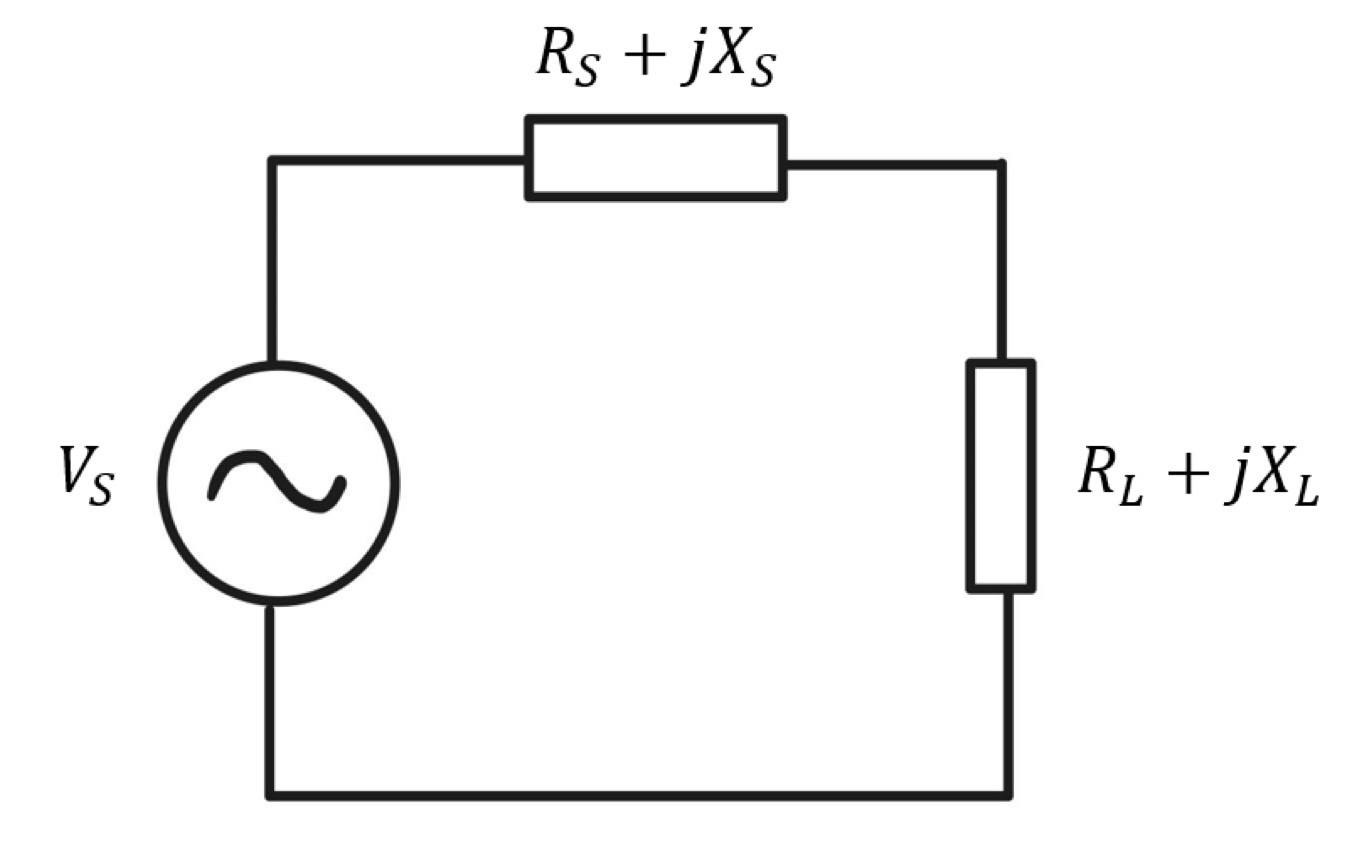
\includegraphics[width=0.4\textwidth]{genpath_elec_cir.jpg}
    \end{center}
    \caption{วงจรสมมูลของวงจรกักเก็บพลังงาน \cite{MPPT}}
    \label{genpath_elec_cir}
\end{figure}
พิจารณาหลักการแมทชิงอิมพีแดนซ์ (Matching impedance) เมื่อพิจารณากำลังออก($P_{out}$) โดยใช้ทฤษฎีการถ่ายโอนกำลังสูงสุด (Maximum Power Transfer) ของวงจรสมมูลดังกล่าว เมื่อโหลดเป็นอิมพีแดนซ์ใดๆ โดยพิจารณาในสภาวะคงตัว (steady state)
\begin{equation}
    S = \frac{|V_{s}|^2 }{ Z^{*} } = \frac{|V_{s}|^2 }{ (R_{s} + R_{L}) - j(X_{s} + X_{L} )  }
\end{equation}
\begin{equation}\label{Pout1}
    P_{out} = Re(S) = \frac{|V_{s}|^2 R_{L} }{ (R_{s} + R_{L})^2 + (X_{s} + X_{L} )^2  }
\end{equation}
เมื่อ

$S$ คือ กำลังปรากฎ

$P_{out}$ คือ กำลังขาออก

จากสมการที่ ({\ref{Pout1}}) จะมีค่าสูงสุดเมื่อพจน์ตัวหารมีค่าต่ำที่สุด เนื่องจากค่ารีแอคแตนซ์สามารถมีค่าน้อยกว่าศูนย์ได้จึงพิจารณาให้ $X_{L} = - X_{g}$ จึงได้
\begin{equation}
    P_{out}  = \frac{|V_{s}|^2 R_{L} }{ (R_{s} + R_{L})^2 }
\end{equation}
และจะได้ว่า $P_{out}$ จะมีค่าสูงสุดเมื่อ $\frac{ R_{L} }{ (R_{s} + R_{L})^2 }$ มีค่าสูงสุด จากนั้นพิจารณาค่า $R_{L}$ ที่ส่งผลให้พจน์ดังกล่าวมีค่าสูงสุดด้วยสมการที่ (\ref{Pout2})
\begin{equation}\label{Pout2}
    \frac{d}{dt} \frac{ R_{L} }{ (R_{s} + R_{L})^2 } = 0
\end{equation}
\begin{equation}
     R_{L} = R_{s} 
\end{equation}


จึงได้ว่า $P_{out}$ จะมีค่าสูงสุดเมื่อ $R_{L} = R_{S}$ และ $j\omega X_{L} = -j\omega X_{S}$ 
ต่อมาจะเป็นจะเป็นการขยายแนวคิดดังกล่าว โดยพิจารณากับสัญญาณกระแส ณ ขณะใดๆ เปลี่ยนแปลงตามเวลา 
เนื่องจากลักษณะโหลดเปลี่ยนแปลงตามค่ากระแส ณ เวลานั้นๆ ซึ่งการเปลี่ยนแปลงโหลดนั้นทำได้ยากในทางปฏิบัติ ดังนั้น
จึงพิจารณาในรูปแรงดันแทน จะได้ว่าแรงดันตกคร่อมโหลดจะต้องมีค่าเท่ากับสังยุคของแรงดันตกคร่อมอิมพีแดนซ์วงจรสมมูลขาออก จะได้

\begin{equation}
    \vec{v}_{load}  = R_{g}
    \begin{bmatrix}
        i_{x} \\i_{y}
    \end{bmatrix} - L_{s}\frac{d}{dt}
    \begin{bmatrix}
        i_{x} \\i_{y}
    \end{bmatrix}
\end{equation}
เนื่องจากโหลดที่ต่ออยู่เป็นแบตเตอรี ถ้าสามารถควบคุมแรงดันขาออก($v_{ter}$) ดังสมการที่ (\ref{vter}) จะทำให้กำลังไปไฟฟ้าที่ชาร์จเข้าแบตเตอรีมีค่าสูงสุด
\begin{equation}\label{vter}
    \vec{v}_{ter} =
    \begin{bmatrix}
        v_{ox} \\v_{oy}
    \end{bmatrix} = R_{g}
    \begin{bmatrix}
        i_{x} \\i_{y}
    \end{bmatrix} - L_{s}\frac{d}{dt}
    \begin{bmatrix}
        i_{x} \\i_{y}
    \end{bmatrix}
\end{equation}
โดยการควบคุมแรงดันขาออกของแบตเตอรีให้เป็นไปตามที่ต้องการตามสมการที่ (\ref{vter}) จะใช้วงจรอินเวอร์เตอร์ในการแปลงแรงดันไฟฟ้า โดยใช้เทคนิคการมอดูเลเลตความกว้างพัลส์

นอกจากนี้ยังต้องคำนึงถึงข้อควรระวังของการใช้ตัวอนุพันธ์ เนื่องจากราฟผลตอบสนองเชิงความถี่ดังรูปที่ \ref{bode_1} เห็นได้ว่าตัวอนุพันธ์มีพฤติกรรมเหมือนตัวขยายสัญญาณ
หากมีสัญญาณรบกวนความถี่สูงเข้ามา อาจทำให้สัญญาณรบกวนถูกขยายขนาดมากขึ้น และอาจส่งผลให้อุปกรณ์เสียหายได้ ดังนั้นการแก้ปัญหาดังกล่าวจึงต้องมีการจำกัดขอบเขตช่วงความถี่
ของตัวอนุพันธ์ดัวยตัวปฏิพันธ์ ซึ่งมีฟังก์ชันถ่ายโอน(Tranfer function) ดังสมการด้านล่าง 
\begin{equation}\label{bode1}
    H(s)  = \frac{ s }{ \frac{s}{\omega_{H}} + 1 }
\end{equation}

\subsection{การดึงกำลังไฟฟ้าสูงสุดที่ได้จากแผ่นพื้นเก็บพลังงานโดยใช้เครื่องจักรกลไฟฟ้ากระแสตรง ด้วยวิธีการติดตามจุดทำงานสูงสุด}
ระบบแผ่นพื้นเก็บพลังงานนั้น แสดงดังรูปที่ \ref{mech_and_dc_motor} ทางฝั่งทางกลประกอบด้วยกลไกเกลียวตัวหนอน (lead screw) และ เกียร์ ส่วนทางฝั่งไฟฟ้ามีเครื่องจักรกลไฟฟ้ากระแสตรงซึ่งมีความต้านทานและค่าความเหนี่ยวตัวตัวเอง ต่ออยู่กับโหลด ($R_{L}$) 
\begin{figure}[H]
    \begin{center}
        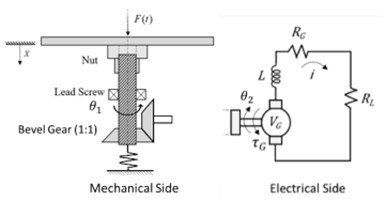
\includegraphics[width=0.4\textwidth]{mech_and_dc_motor.jpg}
    \end{center}
    \caption{ระบบทางกายภายของกลไกเกลียวนำของแผ่นพื้นและเครื่องจักรกลไฟฟ้า}
    \label{mech_and_dc_motor}
\end{figure}

จากนั้นพิจารณาฝั่งทางกลในรูปแบบของวงจรไฟฟ้าโดยใช้การเปรียบเทียบเชิงกล-ไฟฟ้า ดังที่กล่าวไว้ก่อนหน้า จึงได้วงสมมูลของระบบทางกลของแผ่นพื้นเก็บพลังงาน แสดงดังรูปที่ \ref{}
ส่วนวงจรสมูลของเครื่องจักรกลไฟฟ้ากระแสตรง แสดงดังรูปที่ \ref{} โดยมีความต้านทานและความเหนี่ยวนำขดลวดสเตเตอร์รวมอยู่ด้วย
\begin{figure}[H]
    \begin{center}
        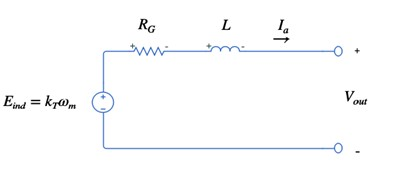
\includegraphics[width=0.5\textwidth]{dc_motor_circuit.jpg}
    \end{center}
    \caption{วงจรสมมูลเครื่องจักรไฟฟ้ากระแสตรง}
    \label{dc_motor_circuit}
\end{figure}
โดยที่

$R_{G}$      คือ ความต้านทานภายในของเครื่องจักรกลไฟฟ้ากระแสตรง

$L$ 	     คือ ความเหนี่ยวนำภายในของเครื่องจักรกลไฟฟ้ากระแสตรง

$E_{ind}$	 คือ แรงเคลื่อนเหนี่ยวนำภายในของเครื่องจักรกลไฟฟ้ากระแสตรง

เมื่อพิจารณาวงจรสมมูลทั้งทางระบบทางกลและทางไฟฟ้า ดังแสดงในรูปที่ \ref{mech_and_dc_motor_circuit} จะพบว่าทั้งสองมีความสัมพันธ์กัน โดยพิจารณาเป็นหม้อแปลงแรงดันที่มีอัตราส่วนจำนวนรอบ คือ $1 : k_{T}$ ดังแสดงในรูปที่ \ref{dc_tr}
\begin{figure}[H]
    \begin{center}
        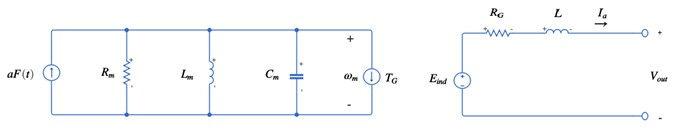
\includegraphics[width=0.8\textwidth]{mech_and_dc_motor_circuit.jpg}
    \end{center}
    \caption{วงจรสมมูลไฟฟ้าของระบบกลของแผ่นพื้นเก็บพลังงานและเครื่องจักรไฟฟ้ากระแสตรง}
    \label{mech_and_dc_motor_circuit}
\end{figure}
\begin{figure}[H]
    \begin{center}
        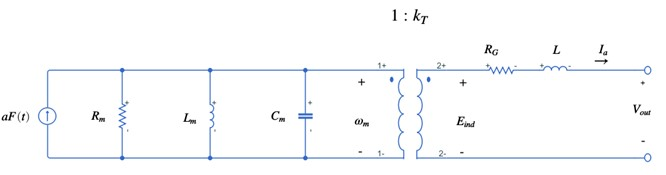
\includegraphics[width=0.8\textwidth]{dc_tr.jpg}
    \end{center}
    \caption{วงจรไฟฟ้าแสดงความสัมพันธ์ระบบทางกลและเครื่องจักรกลไฟฟ้ากระแสตรงผ่านหม้อแปลงไฟฟ้าที่มีอัตราส่วนจำนวน คือ $1 : k_{T}$}
    \label{dc_tr}
\end{figure}
จากนั้นอ้างอิงวงจรทางด้านทุติยภูมิของหม้อแปลง (ด้านเครื่องจักรไฟฟ้ากระแสตรง) จึงได้วงจร ดังแสดงในรูปที่ \ref{genpath_cicuit} 
\begin{figure}[H]
    \begin{center}
        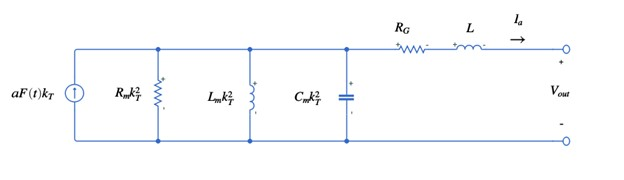
\includegraphics[width=0.8\textwidth]{genpath_circuit.jpg}
    \end{center}
    \caption{วงจรสมมูลไฟฟ้าของแผ่นพื้นเก็บพลังงาน}
    \label{genpath_cicuit}
\end{figure}
สัญญาณของระบบมาจากเท้าเหยียบของมนุษย์ ซึ่งเป็นสัญญาณที่ไม่เป็นรายคาบ และแปรเปลี่ยนไปตามเวลา การดึงกำลังสูงสุดจากวงจรจึงพิจารณาทฤษฎีกำลังถ่ายโอนสูงสุดของระบบพลวัตไม่เป็นเชิงเส้น (Nonlinear Dynamic Maximum Power Transfer Theorem, ND-MPTT) ซึ่งเป็นทฤษฎีที่พิจารณากรณีทั่วไปกว่าทฤษฎี การถ่ายโอนกำลังสูงสุด (Maximum Power Transfer Theorem, MPTT)  
โดยวงจรแผ่นพื้นเก็บพลังงานในรูปที่ แสดงในลาปลาสโดเมนดังรูปที่ \ref{laplce_genpath_circuit} ที่ได้จากการใช้ทฤษฎีของเทเวนินในการแปลงวงจร 
\begin{figure}[H]
    \begin{center}
        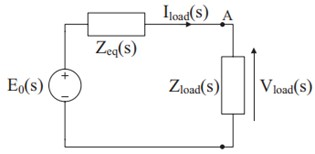
\includegraphics[width=0.4\textwidth]{laplce_genpath_circuit.jpg}
    \end{center}
    \caption{วงจรสมมูลของแผ่นพื้นเก็บพลังงานในลาปลาสโดเมน}
    \label{laplce_genpath_circuit}
\end{figure}
\begin{equation}\label{zeq}
    Z_{eq}  = R_{G} + sL + \frac{ sR'_{m}L'_{m} }{ s^2R'_{m}L'_{m}C'_{m} + sL'_{m} + R'_{m} }
\end{equation}
โดยที่

$R'_{m} = \frac{R_{m}}{k_{t}^2}$, $L'_{m} = \frac{L_{m}}{k_{t}^2}$,และ $C'_{m} = \frac{C_{m}}{k_{t}^2}$

$E_{0} = V_{load}(s)\vert_{I_{load}(s) = 0} = -I_{f}(s) \cdot \frac{ sR'_{m}L'_{m} }{ s^2R'_{m}L'_{m}C'_{m} + sL'_{m} + R'_{m}}$
\begin{equation}\label{E0}
    E_{0} = -F(s) \cdot ak_{T} \cdot \frac{ sR'_{m}L'_{m} }{ s^2R'_{m}L'_{m}C'_{m} + sL'_{m} + R'_{m}}
\end{equation}
ทฤษฎีกำลังถ่ายโอนสูงสุดของระบบพลวัตไม่เป็นเชิงเส้น กล่าวว่า กำลังที่ดึงได้สูงสุดจากวงจรแผ่นพื้นเก็บพลังงาน เมื่อสัญญาณขาเข้าเป็นสัญญาณใดๆ จะได้ว่า อิมพีแดนซ์ที่เหมาะสมของอิมพีแดนซ์ของโหลด คือ
$Z_{opt}(s)= Z_{eq}(-s)$

\textbf{ข้อสังเกต}

หากสัญญาณขาเข้าเป็นสัญญาณเป็นไซน์นูซอยด์ที่ความที่ $\omega = \omega_{res} = \frac{1}{\sqrt{L'_{m}C'_{m}}}$ แล้ว 
ค่า $ L'_{m} $ และ $ C'_{m} $ จะถูกชดเชยอย่างสมบูรณ์ ดังวงจรแสดงในรูปที่ \ref{genpath_cicuit} ดังนั้น จากสมการ \ref{zeq} และ \ref{E0} จะได้

\begin{equation} 
    Z_{eq}\vert_{s = j\omega_{res}} = (R_{G} + sL + R_{m} )\vert_{s = j\omega_{res}}
\end{equation}

\begin{equation}
    E_{0}\vert_{s = j\omega_{res}} = -F(s) \cdot ak_{T} \cdot R'_{m}
\end{equation}
ดังนั้น การประยุกต์ใช้งาน ND-MPPT ในสัญญาณไซด์นูซอยด์ ที่ความถี่เรโซแนนท์ $\omega = \omega_{res}$ จะได้ผลลัพธ์ คือ
\begin{equation}
    Z_{opt}\vert_{s = j\omega_{res}} = Z_{eq}(-s)\vert_{s = j\omega_{res}} = -F(s) \cdot ak_{T} \cdot R'_{m} \vert_{s = j\omega_{res}} = conj [ {\dot{ Z_{eq} } (j\omega_{res})} ] 
\end{equation}
จากสมการนั้นหมายความว่าในกรณีสัญญาณไซด์นูซอยด์ ที่ความถี่เรโซแนนท์ จะทำให้ได้เงื่อนไขโหลดของทั้ง ND-MPPT และ MPPT จะเหมือนกัน 

หากระบบแผ่นพื้นเก็บพลังงานได้รับการออกแบบอย่างดีให้มี Q factor สูง จะทำให้แถบ 3dB นั้นแคบ และสัญญาณขาเข้าของระบบไม่เป็นสัญญาณไซน์ที่เปลี่ยนแปลงตามเวลา 
จะทำให้ได้แรงดันเปิดวงจร $E_{0}$ จะมีสัญญาณที่ใกล้เคียงสัญญาณไซน์ที่ความถี่ $\omega = \omega_{res}$ ดังนั้น ระบบแผ่นพื้นกักเก็บพลังงานที่มี Q factor สูง ส่งผลให้ MPPT และ ND-MPPT ได้เงื่อนไขโหลดที่เหมาะสมเหมือนกัน คือ
\begin{equation} \label{}
    Z_{opt}(s)= Z_{eq}(-s) \cong R_G- sL+ R'_{m}  
\end{equation}

\newpage

\section{ผลลัพธ์จากการดำเนินการเบื้องต้น}

\subsection{การทดสอบอัลกอริทึมการมอดูเลตแบบสองแขน และการติดตามการทำงานในจตุภาคที่หนึ่ง}

ในการทดสอบอัลกอริทึมการมอดูเลตแบบสองแขน และการติดตามการทำงานในจตุภาคที่หนึ่ง จะทำโดยการนำอินเวอร์เตอร์ไปต่อกับโหลดแบบตัวต้านทานและตัวเหนี่ยวนำสามเฟส โดยเราจะทดลองปรับค่าคำสั่งต่างๆของอินเวอร์เตอร์ และดูว่าระบบให้ผลตอบสนองที่ถูกต้องหรือไม่ อัลกอริทึมมีการตัดสินใจที่ถูกต้องหรือไม่ โหมดในการทำงานสอดคล้องกับสิ่งที่เกิดขึ้นจริงหรือไม่ โดยการประเมินผลที่ได้กล่าวข้างต้น จะต้องมีการวัดและแสดงค่าต่างๆ เหล่านี้คือ

\begin{itemize}
    \item ค่าแรงดันเฟสคำสั่งของอินเวอร์เตอร์ (Commanded Phase Voltage)
    \item กระแสสายของอินเวอร์เตอร์ที่วัดได้ (Line Current)
    \item โหมดการมอดูเลตแบบสองแขนที่อัลกอริทึมตัดสินใจเลือก (Two Arm Modulator Command Mode; TAM Command Mode)
    \item แรงดันคำสั่งที่คำนวนได้จากอัลกอริทึม (Two Arm modulator and First Quadrant Tracker Output; TAM \& FQT Output)
\end{itemize}

\begin{figure}[H]
    \centering
    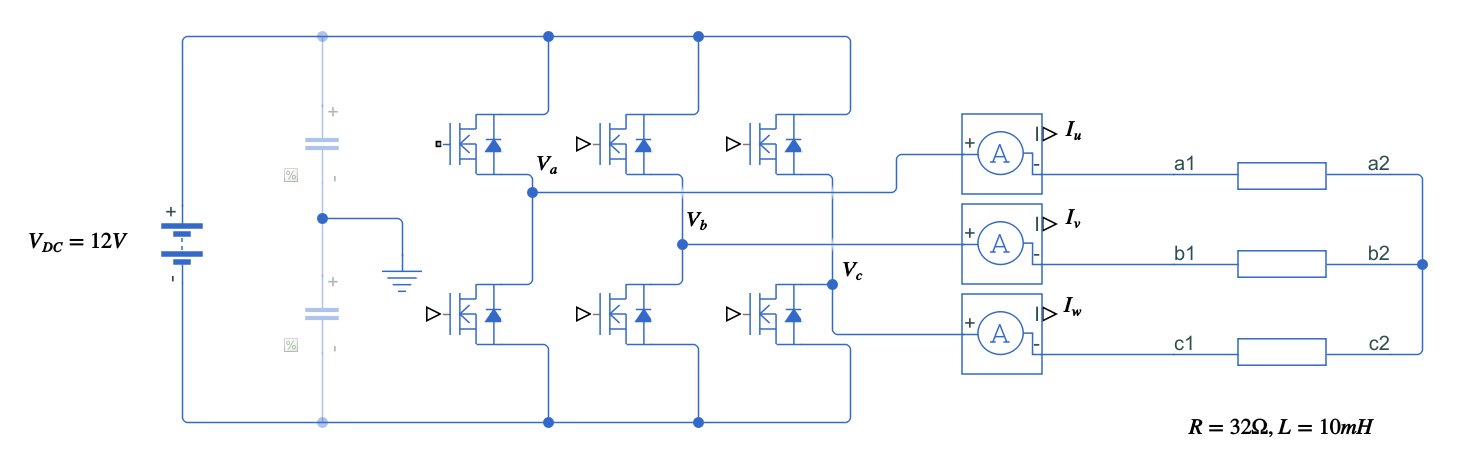
\includegraphics[width=\textwidth]{ildef.png}
    \caption{รูปแบบวงจรที่ใช้ทดสอบอัลกอริทึมการมอดูเลตแบบสองแขน และการติดตามการทำงานในจตุภาคที่หนึ่ง}
    \label{ildef}
\end{figure}

ค่าแรงดันเฟสคำสั่งของอินเวอร์เตอร์ จะเป็นค่าแรงดันที่ป้อนให้กับอัลกอริทึมของอินเวอร์เตอร์ \newline ค่ากระแสสาย จะนิยามตามรูปที่ \ref{ildef} คือ นิยามให้กระแสที่ไหลออกจากขั้วของอินเวอร์เตอร์เป็นค่าบวก \newline โหมดการมอดูเลตแบบสองแขนที่อัลกอริทึมตัดสินใจเลือก จะเป็นโหมดที่ได้กล่าวไว้ในรายละเอียดของการมอดูเลตแบบสองแขนคือ

\begin{itemize}
    \item Upper จะเป็นโหมดที่เลือกให้สวิตช์ตัวที่นำกระแสตลอดเวลาเป็นทรานซิสเตอร์ตัวบน
    \item Lower จะเป็นโหมดที่เลือกให้สวิตช์ตัวที่นำกระแสตลอดเวลาเป็นทรานซิสเตอร์ตัวล่าง
    \item Both จะเป็นโหมดที่เลือกให้ทรานซิสเตอร์ตัวบน หรือตัวล่างนำกระแสตลอดเวลาก็ได้ ขึ้นกับว่าทรานซิสเตอร์ตัวไหนทำงานหนักว่า โดยจะแบ่งงานกันทำระหว่างทรานซิสเตอร์ตัวบนและตัวล่าง
\end{itemize}

แรงดันคำสั่งที่คำนวนได้จากอัลกอริทึม คือ แรงดันที่คำนวนได้หลังจากการตัดสินใจว่าต้องการมอดูเลตสองแขนแบบไหน โดยจะทำการเลือกแรงดันลำดับศูนย์เพื่อที่จะบวกเข้าไปในแต่ละเฟส เพื่อให้สวิตช์นำกระแสในแบบที่อัลกอริทึมต้องการ

\subsubsection{เงื่อนไขการทดสอบกรณีที่ปรับความถี่คำสั่งของอินเวอร์เตอร์}

\begin{figure}[H]
    \centering
    \includegraphics[width=\textwidth]{25Hz.eps}
    \caption{ผลการทดลองของระบบอินเวอร์เตอร์ที่ความถี่คำสั่งเท่ากับ 25Hz}
    \label{25Hz}
\end{figure}

จากรูปที่ \ref{25Hz} จะเห็นได้ว่า การเหลื่อมกันของกระแสและแรงดันมีค่าน้อยมาก ซี่งเวลาที่กระแสและแรงดันเหลื่อมกันมีค่าต่ำกว่าคาบเวลาการสุ่มและคงค่าของระบบฝังตัว ดังนั้นระบบจึงไม่รับรู้ถึงการเหลื่อมกันของกระแสและแรงดัน ดังนั้น สวิตช์จะทำงานในจุตภาคที่หนึ่งตลอดเวลา ไม่ว่าจะมอดูเลตแบบสองแขนแบบใดก็ตาม ดังที่แสดงในกราฟ โหมดการมอดูเลตแบบสองแขนที่อัลกอริทึมตัดสินใจเลือก จึงเป็นแบบ Both ตลอดเวลา เพราะจากมุมมองของอินเวอร์เตอร์ อัลกอริทึมจะคิดว่าสามารถที่จะมอดูเลตสองแขนแบบใดก็ได้ ดังนั้น ระบบจะมอดูเลตแบบสองแขนสลับกันระหว่างตัวบนนำกระแสตลอด และตัวล่างนำกระแสตลอด โดยมีจุดที่แบ่งการทำงานกันระหว่างทรานซิสเตอร์ตัวบนและตัวล่างอยู่ที่เวลา 0.025 วินาที เพื่อไม่ให้ทรานซิสเตอร์ฝั่งใดทำงานหนักเกินไป

\begin{figure}[H]
    \centering
    \includegraphics[width=\textwidth]{50Hz.eps}
    \caption{ผลการทดลองของระบบอินเวอร์เตอร์ที่ความถี่คำสั่งเท่ากับ 50Hz}
    \label{50Hz}
\end{figure}

จากรูปที่ \ref{50Hz} จะเห็นได้ว่า เมื่อเราเพิ่มความถี่คำสั่งให้กับอินเวอร์เตอร์ จะทำให้ความถี่ไฟฟ้าของแรงดันออกจากอินเวอร์เตอร์มีค่ามากขึ้น ทำให้องค์ประกอบความเหนี่ยวนำของโหลดมีค่ามากขึ้น ทำให้การเหลื่อมกันของกระแสและแรงดันมากขึ้น จึงมีช่วงจังหวะเวลาระหว่างที่แรงดันคำเฟสคำสั่งของอินเวอร์เตอร์ตัดศูนย์ (เปลี่ยนเครื่องหมายจากลบเป็นบวก) และเวลาที่ค่ากระแสสายตัดศูนย์ (เปลี่ยนเครื่องหมายจากลบเป็นบวก) ในช่วงเวลาดังกล่าว แรงดันเฟสคำสั่งจะมีค่าเป็นบวก ส่วนค่ากระแสจะมีค่าเป็นลบ ดังนั้น ถ้าหากเรามอดูเลตแบบทรานซิสเตอร์ตัวบนนำกระแสตลอดเวลา เท่ากับเราบังคับให้กระแสไหลผ่านทรานซิสเตอร์ตัวบน ทำให้ทรานซิสเตอร์ตัวบนทำงานในจตุภาคที่สาม ซึ่งเป็นสิ่งที่ไม่ต้องการ เนื่องจากจะมีแรงดันตกคร่อมทรานซิสเตอร์มากกว่า ดังนั้น เราจึงต้องเลือกให้อัลกอริทึมมอดูเลตแบบสองแขนเลือกมอดูเลตแบบทรานซิสเตอร์ตัวล่างนำกระแสตลอดเวลา ทำให้กระแสไหลผ่านทรานซิสเตอร์ตัวล่างแบบที่จะทำให้ทรานซิสเตอร์ตัวล่างนำกระแสในจตุภาคที่หนึ่ง ซึ่งมีแรงดันตกคร่อมทรานซิสเตอร์น้อยกว่า กำลังสูญเสียระหว่างนำกระแสน้อยกว่า ดังที่จะสะท้อนออกมาในกราฟโหมดการมอดูเลตแบบสองแขนที่อัลกอริทึมตัดสินใจเลือก จะสังเกตุได้ว่า อัลกอริทึมจะเลือกให้อินเวอร์เตอร์มอดูเลตแบบ "Lower" เมื่ออยู่ในช่วงเวลาระหว่างที่ค่าแรงดันเฟสคำสั่งเปลี่ยนเครื่องหมายจากบวกไปลบ และค่าแรงดันสายเปลี่ยนเครื่องหมายจากบวกไปลบ และอัลกอริทึมจะเลือกมอดูเลตแบบ "Upper" ในช่วงเวลาระหว่างที่ค่าแรงดันเฟสคำสั่งเปลี่ยนเครื่องหมายจากลบไปบวก และค่ากระแสสายเปลี่ยนเครื่องหมายจากลบไปบวก ซึ่งหากพิจารณาจากผลการจำลองจะพบว่า อัลกอริทึมได้ทำงานอย่างถูกต้อง

\begin{figure}[H]
    \centering
    \includegraphics[width=\textwidth]{100Hz.eps}
    \caption{ผลการทดลองของระบบอินเวอร์เตอร์ที่ความถี่คำสั่งเท่ากับ 100Hz}
    \label{100Hz}
\end{figure}

จากรูปที่ \ref{100Hz} จะเห็นได้ว่า เมื่อเราเพิ่มความถี่คำสั่งให้กับอินเวอร์เตอร์ แนวโน้มของการเหลื่อมกันของกระแสและแรงดันจะมีมากขึ้น ดังนั้น ส่วนแบ่งเวลาที่อัลกอริทึมเลือกมอดูเลตแบบ "Upper" และ "Lower" จึงมีมากขึ้น ดังที่จะสะท้อนออกมาในกราฟโหมดการมอดูเลตแบบสองแขนที่อัลกอริทึมเลือก

\subsubsection{เงื่อนไขการทดสอบกรณีที่ปรับค่าความเหนี่ยวนำของโหลด}

จะเห็นได้ว่าการปรับค่าความเหนี่ยวนำของโหลดส่งผลคล้ายกับการปรับค่าความถี่คำสั่งให้กับอินเวอร์เตอร์ เพราะสุดท้ายแล้ว การปรับความถี่คำสั่งของอินเวอร์เตอร์ก็คือการเปลี่ยนค่ารีแอกแตนซ์ของตัวเหนี่ยวนำนั่นเอง จะเห็นได้ว่าอินเวอร์เตอร์สามารถทำงานได้อย่างถูกต้องในกรณีการทดสอบต่างๆ

\begin{figure}[H]
    \centering
    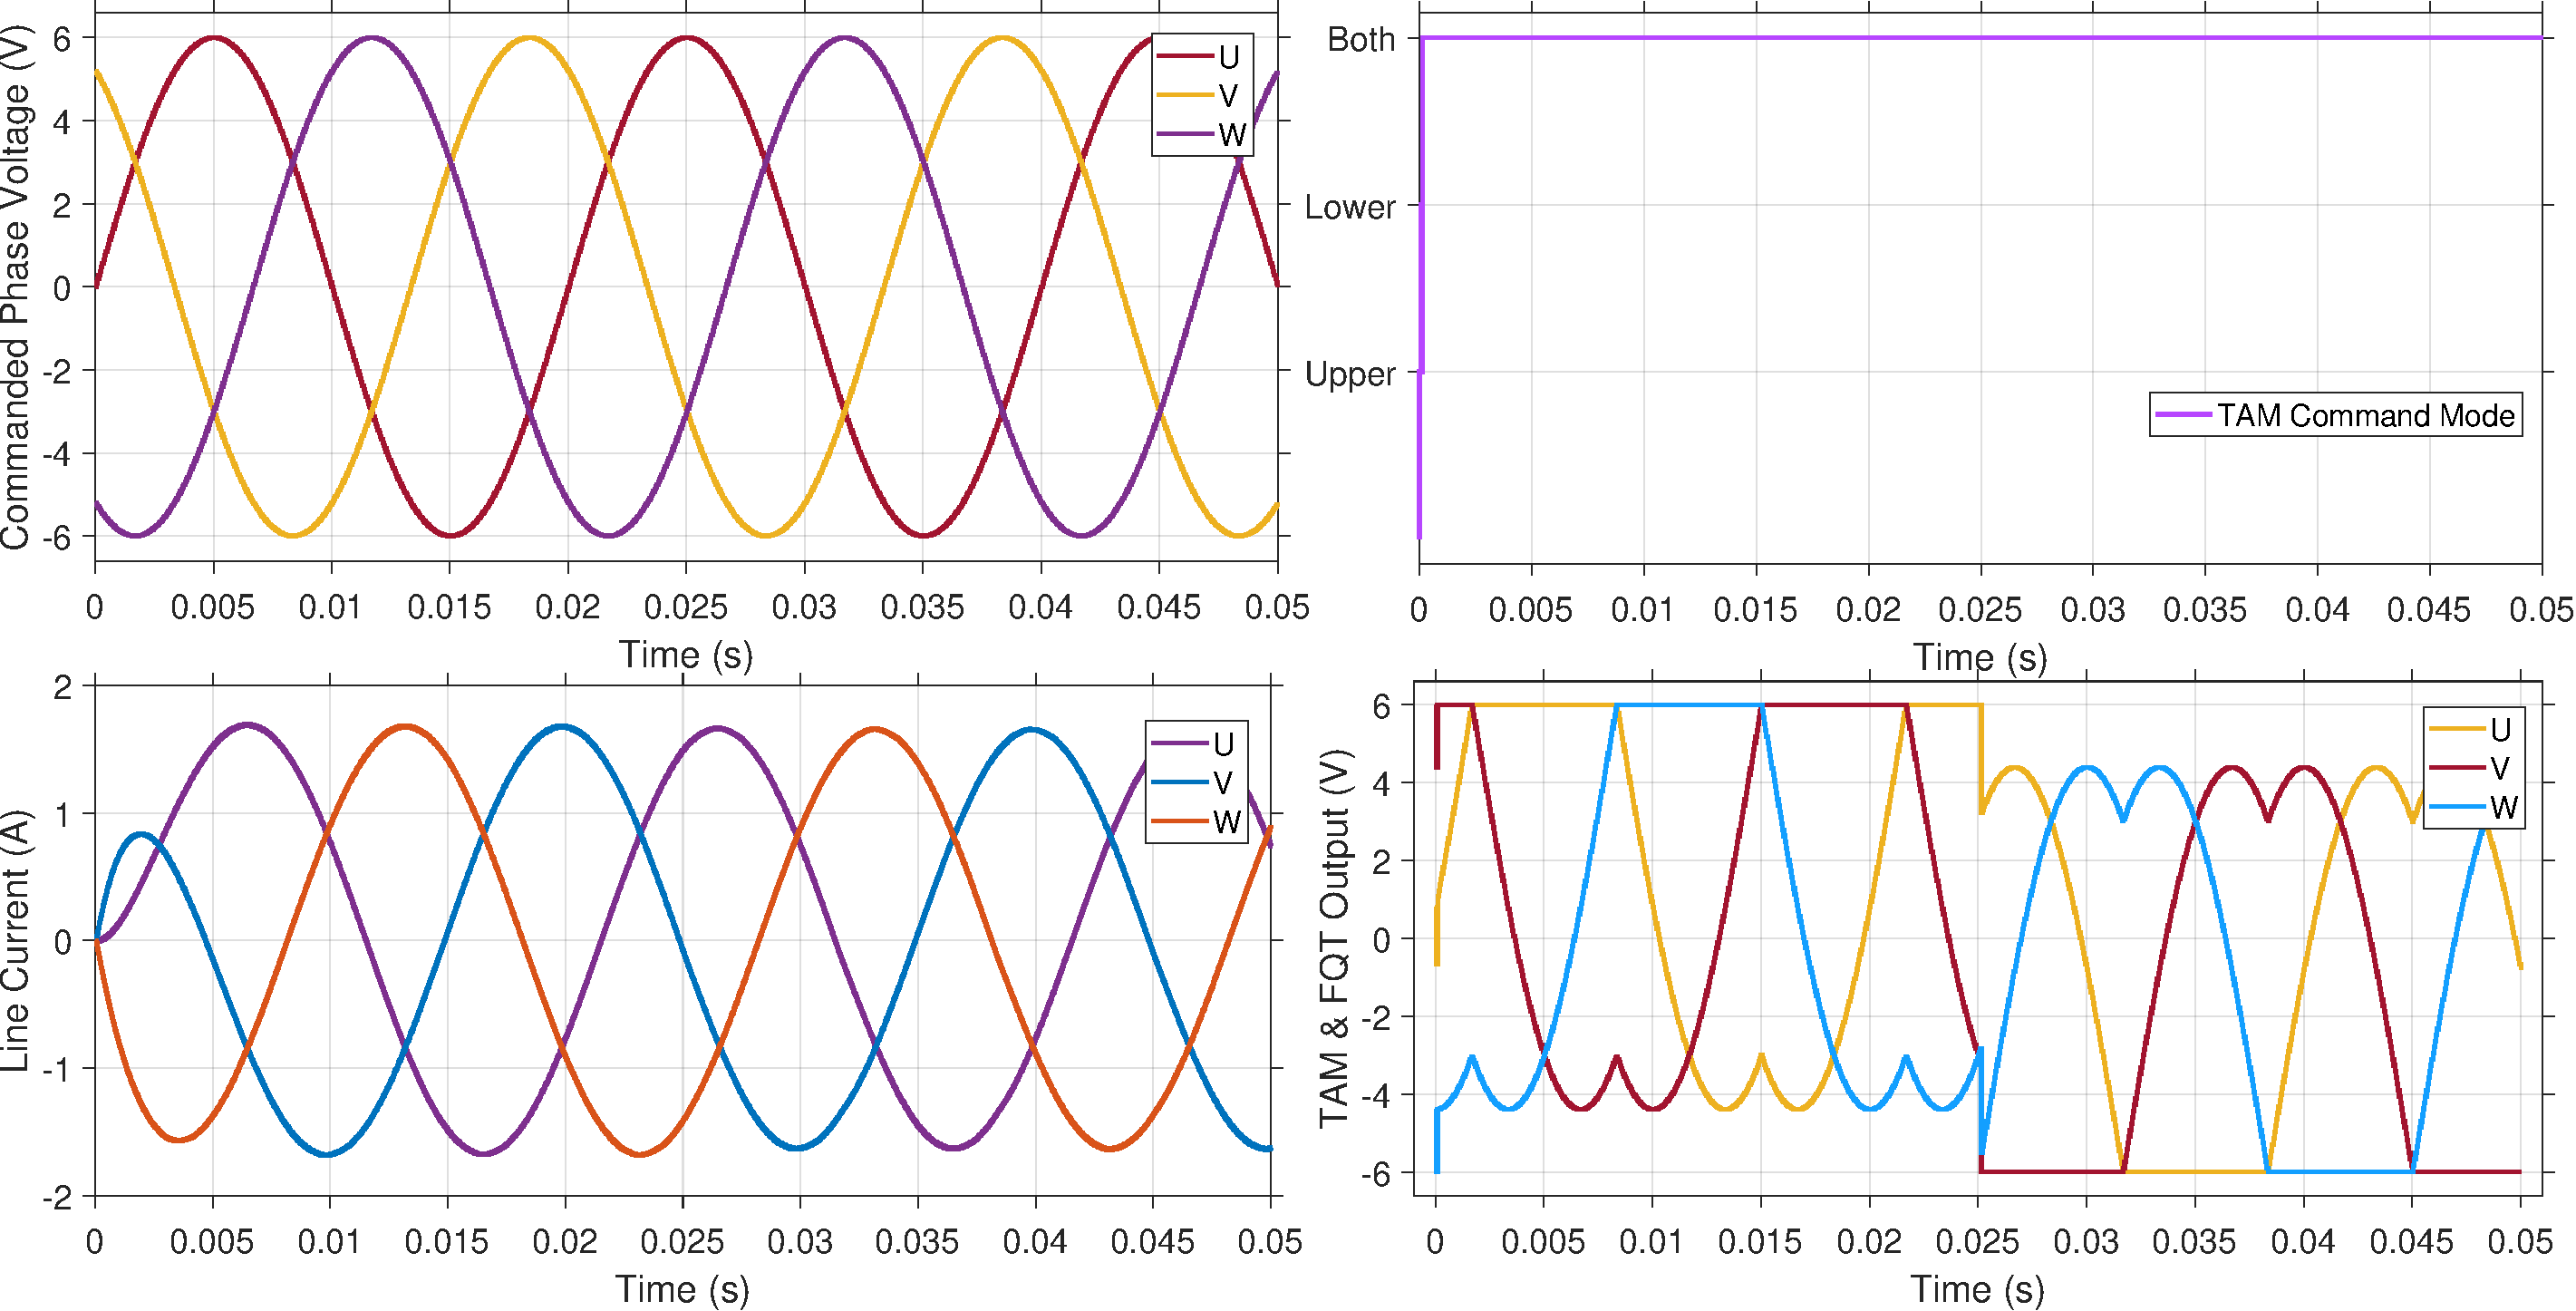
\includegraphics[width=\textwidth]{5mH.pdf}
    \caption{ผลการทดลองของระบบอินเวอร์เตอร์ที่ปรับความเหนี่ยวนำของโหลดให้เท่ากับ 5mH}
    \label{5mH}
\end{figure}

\begin{figure}[H]
    \centering
    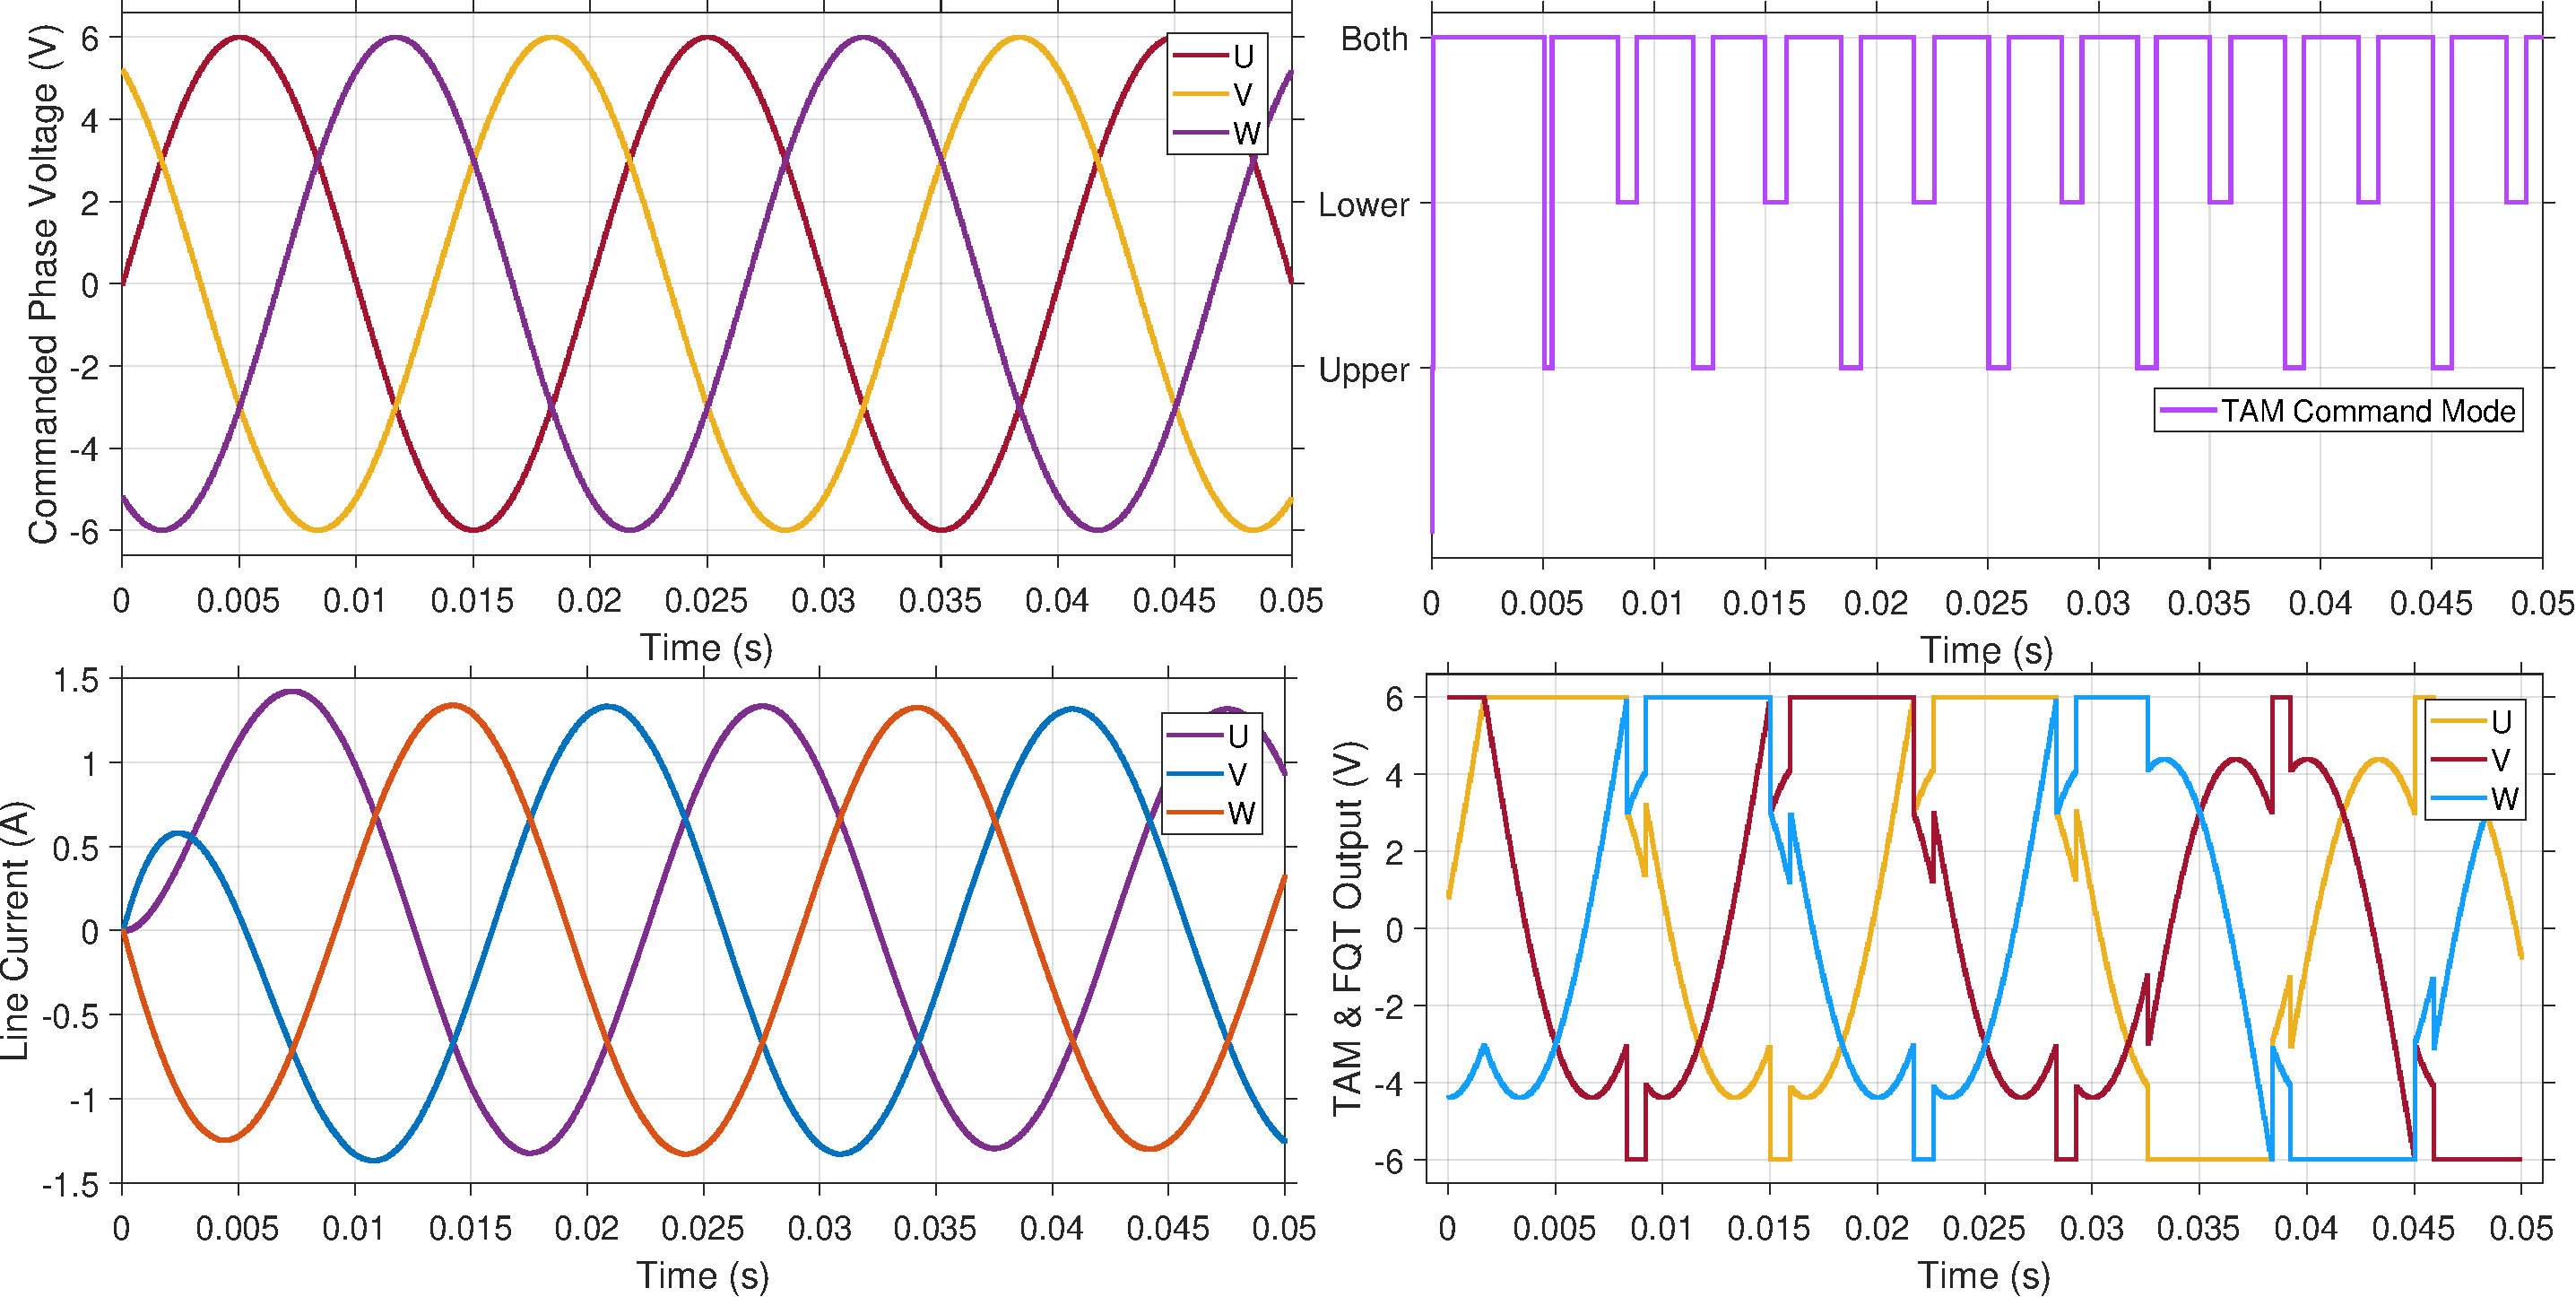
\includegraphics[width=\textwidth]{10mH.pdf}
    \caption{ผลการทดลองของระบบอินเวอร์เตอร์ที่ปรับความเหนี่ยวนำของโหลดให้เท่ากับ 10mH}
    \label{10mH}
\end{figure}

\begin{figure}[H]
    \centering
    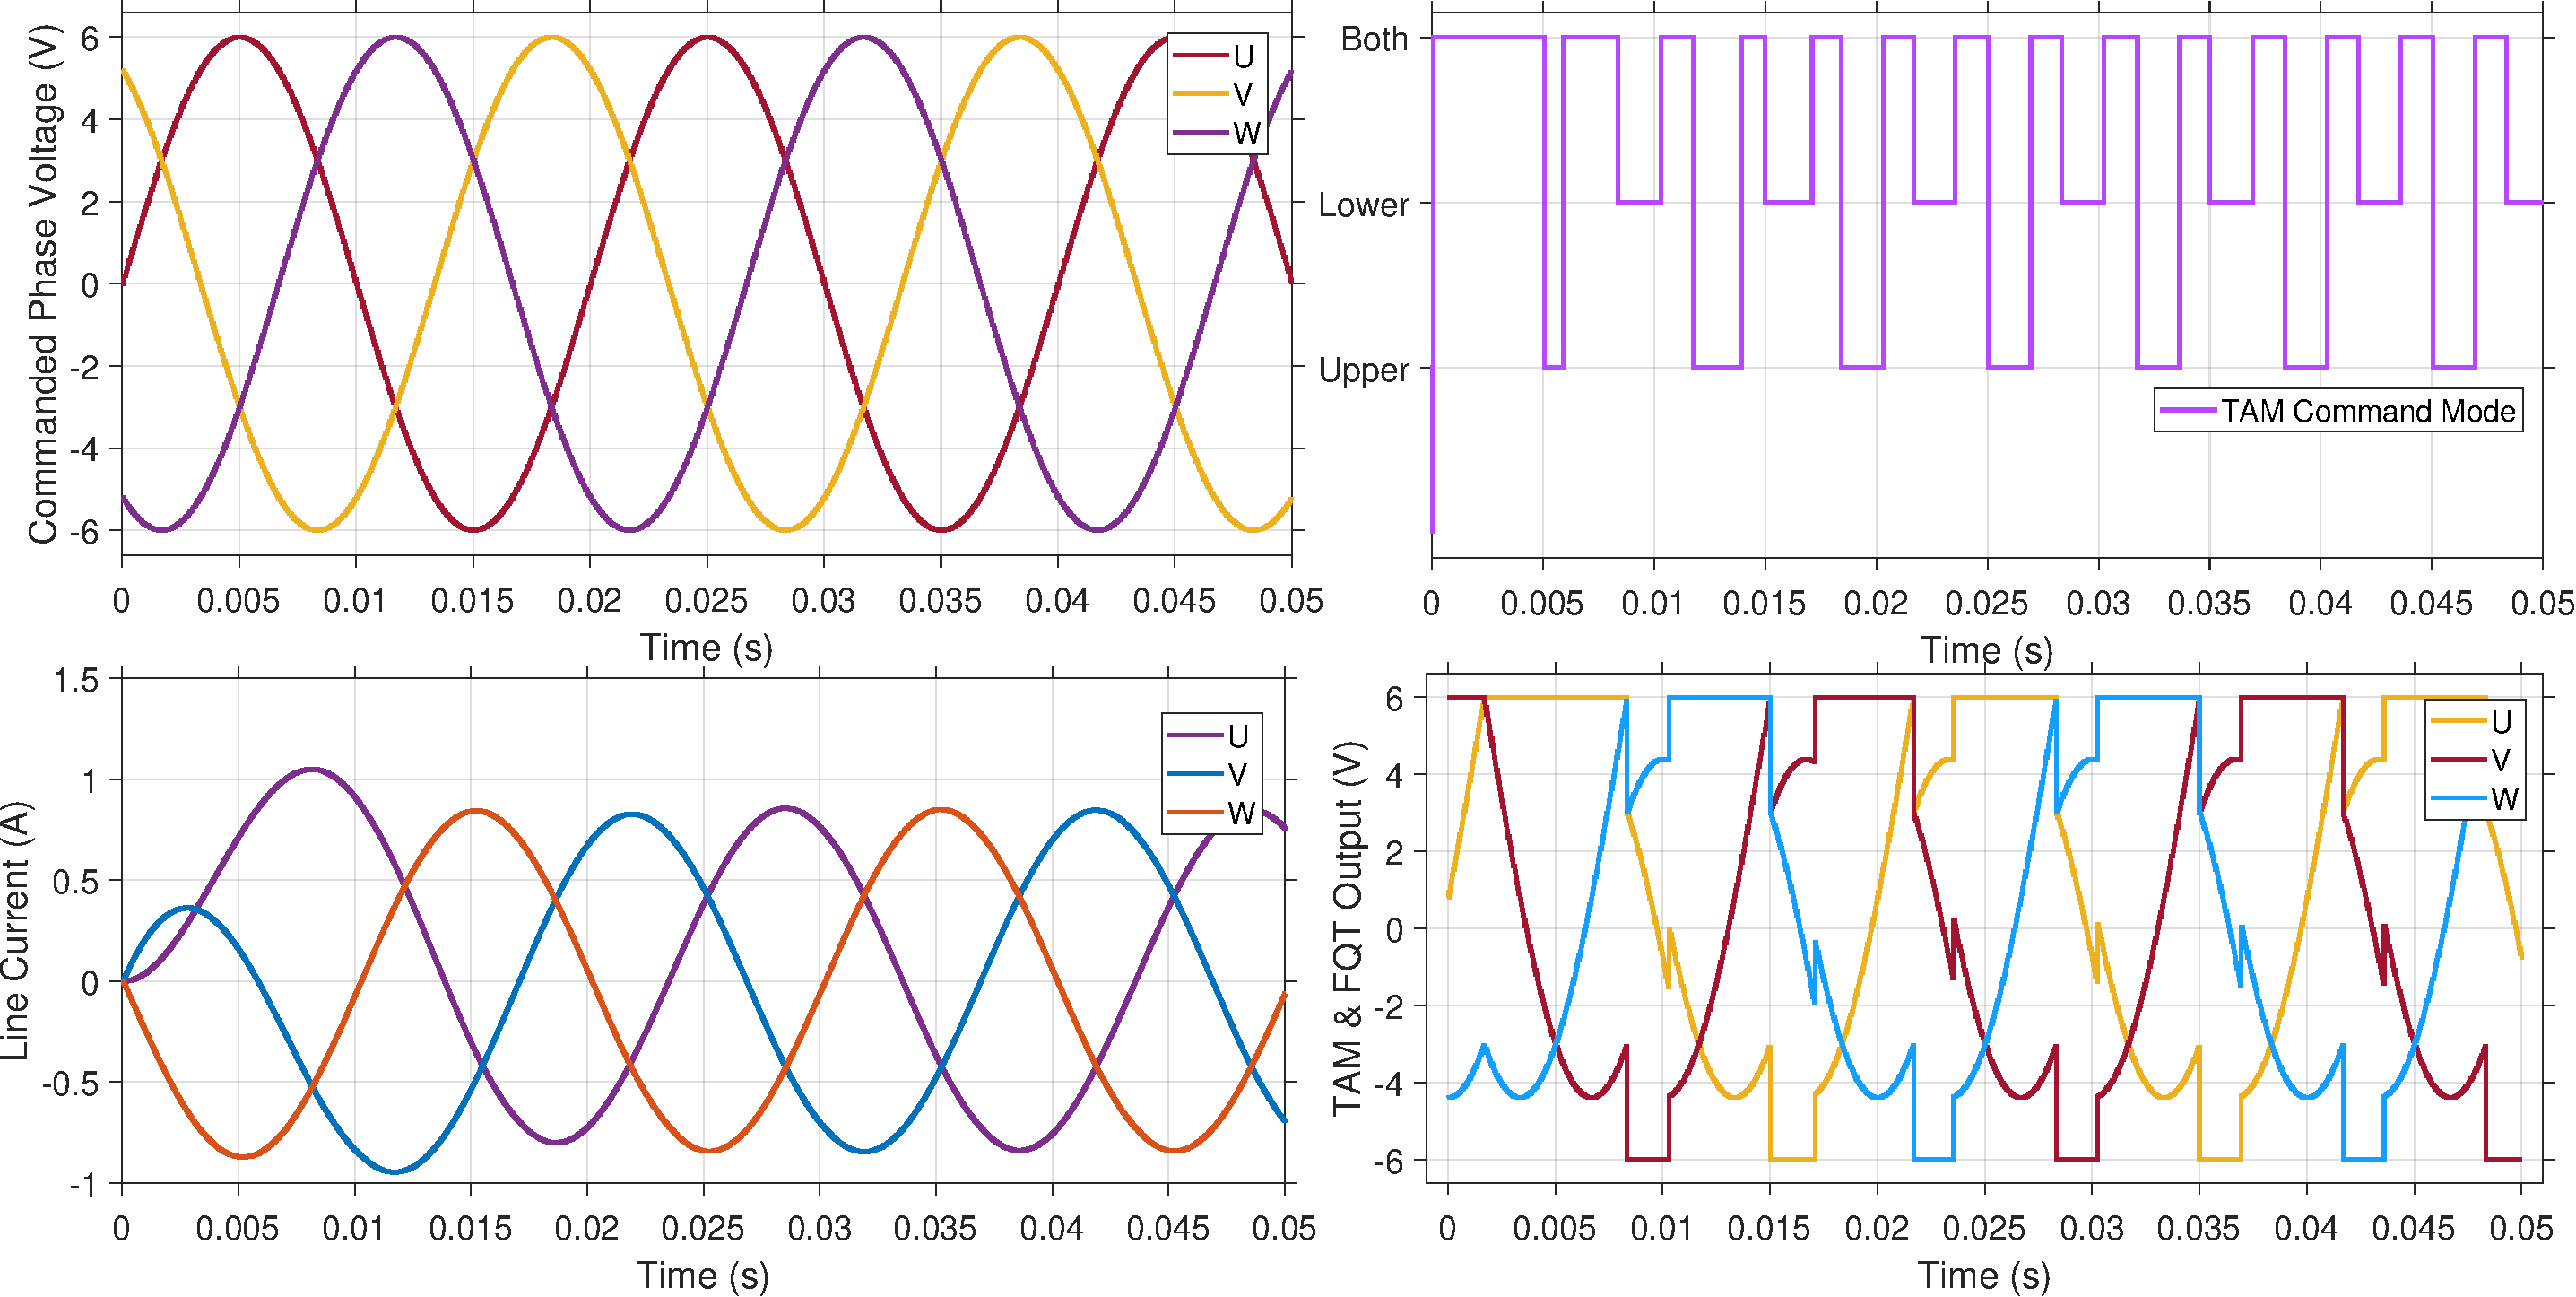
\includegraphics[width=\textwidth]{20mH.pdf}
    \caption{ผลการทดลองของระบบอินเวอร์เตอร์ที่ปรับความเหนี่ยวนำของโหลดให้เท่ากับ 20mH}
    \label{20mH}
\end{figure}

\subsubsection{เงื่อนไขการทดสอบกรณีที่ปรับค่าขนาดของแรงดันคำสั่งของอินเวอร์เตอร์}

ถ้าหากค่ายอดของแรงดันเฟสคำสั่งถูกปรับ ก็จะส่งผลกระทบโดยตรงต่อขนาดของกระแสสาย นั่นคือ ค่ากระแสสายจะแปรผันตรงกับขนาดของแรงดันคำสั่ง จะสังเกตุได้ว่า อินเวอร์เตอร์ยังสามารถทำงานได้ถูกต้องเมื่อปรับขนาดของแรงดันคำสั่งเป็นค่าต่างๆ

\begin{figure}[H]
    \centering
    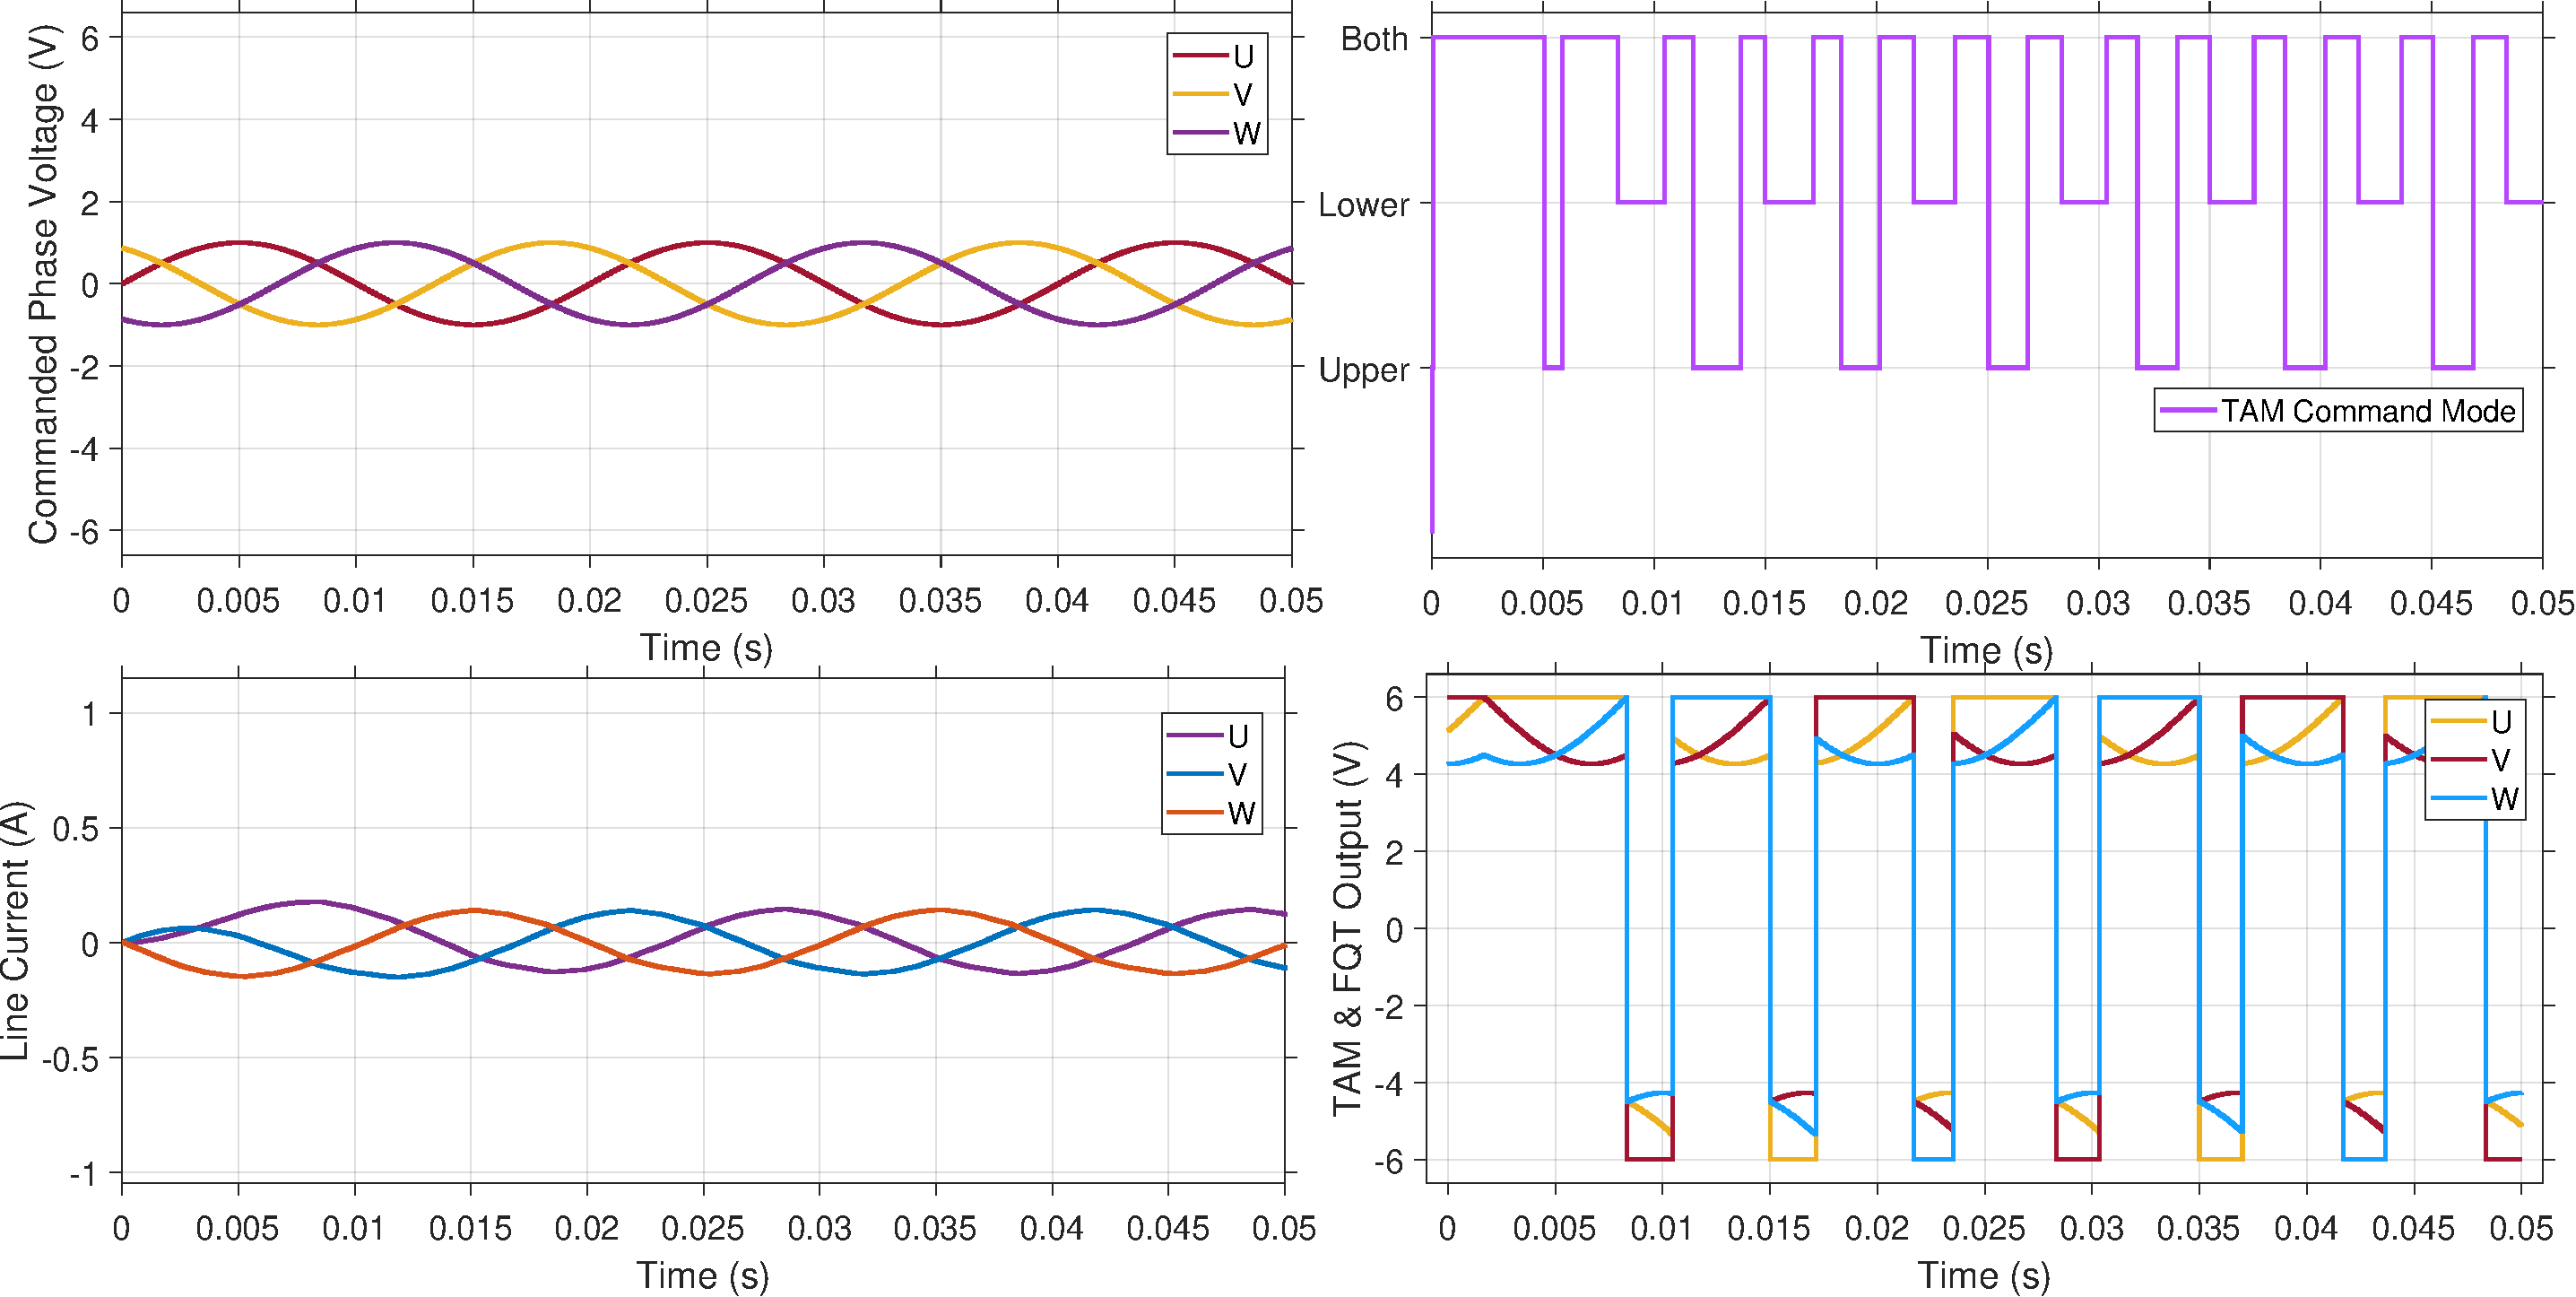
\includegraphics[width=\textwidth]{1V.pdf}
    \caption{ผลการทดลองของระบบอินเวอร์เตอร์ที่ปรับขนาดของค่ายอดของดันเฟสคำสั่งเท่ากับ 1 V}
    \label{1V}
\end{figure}

\begin{figure}[H]
    \centering
    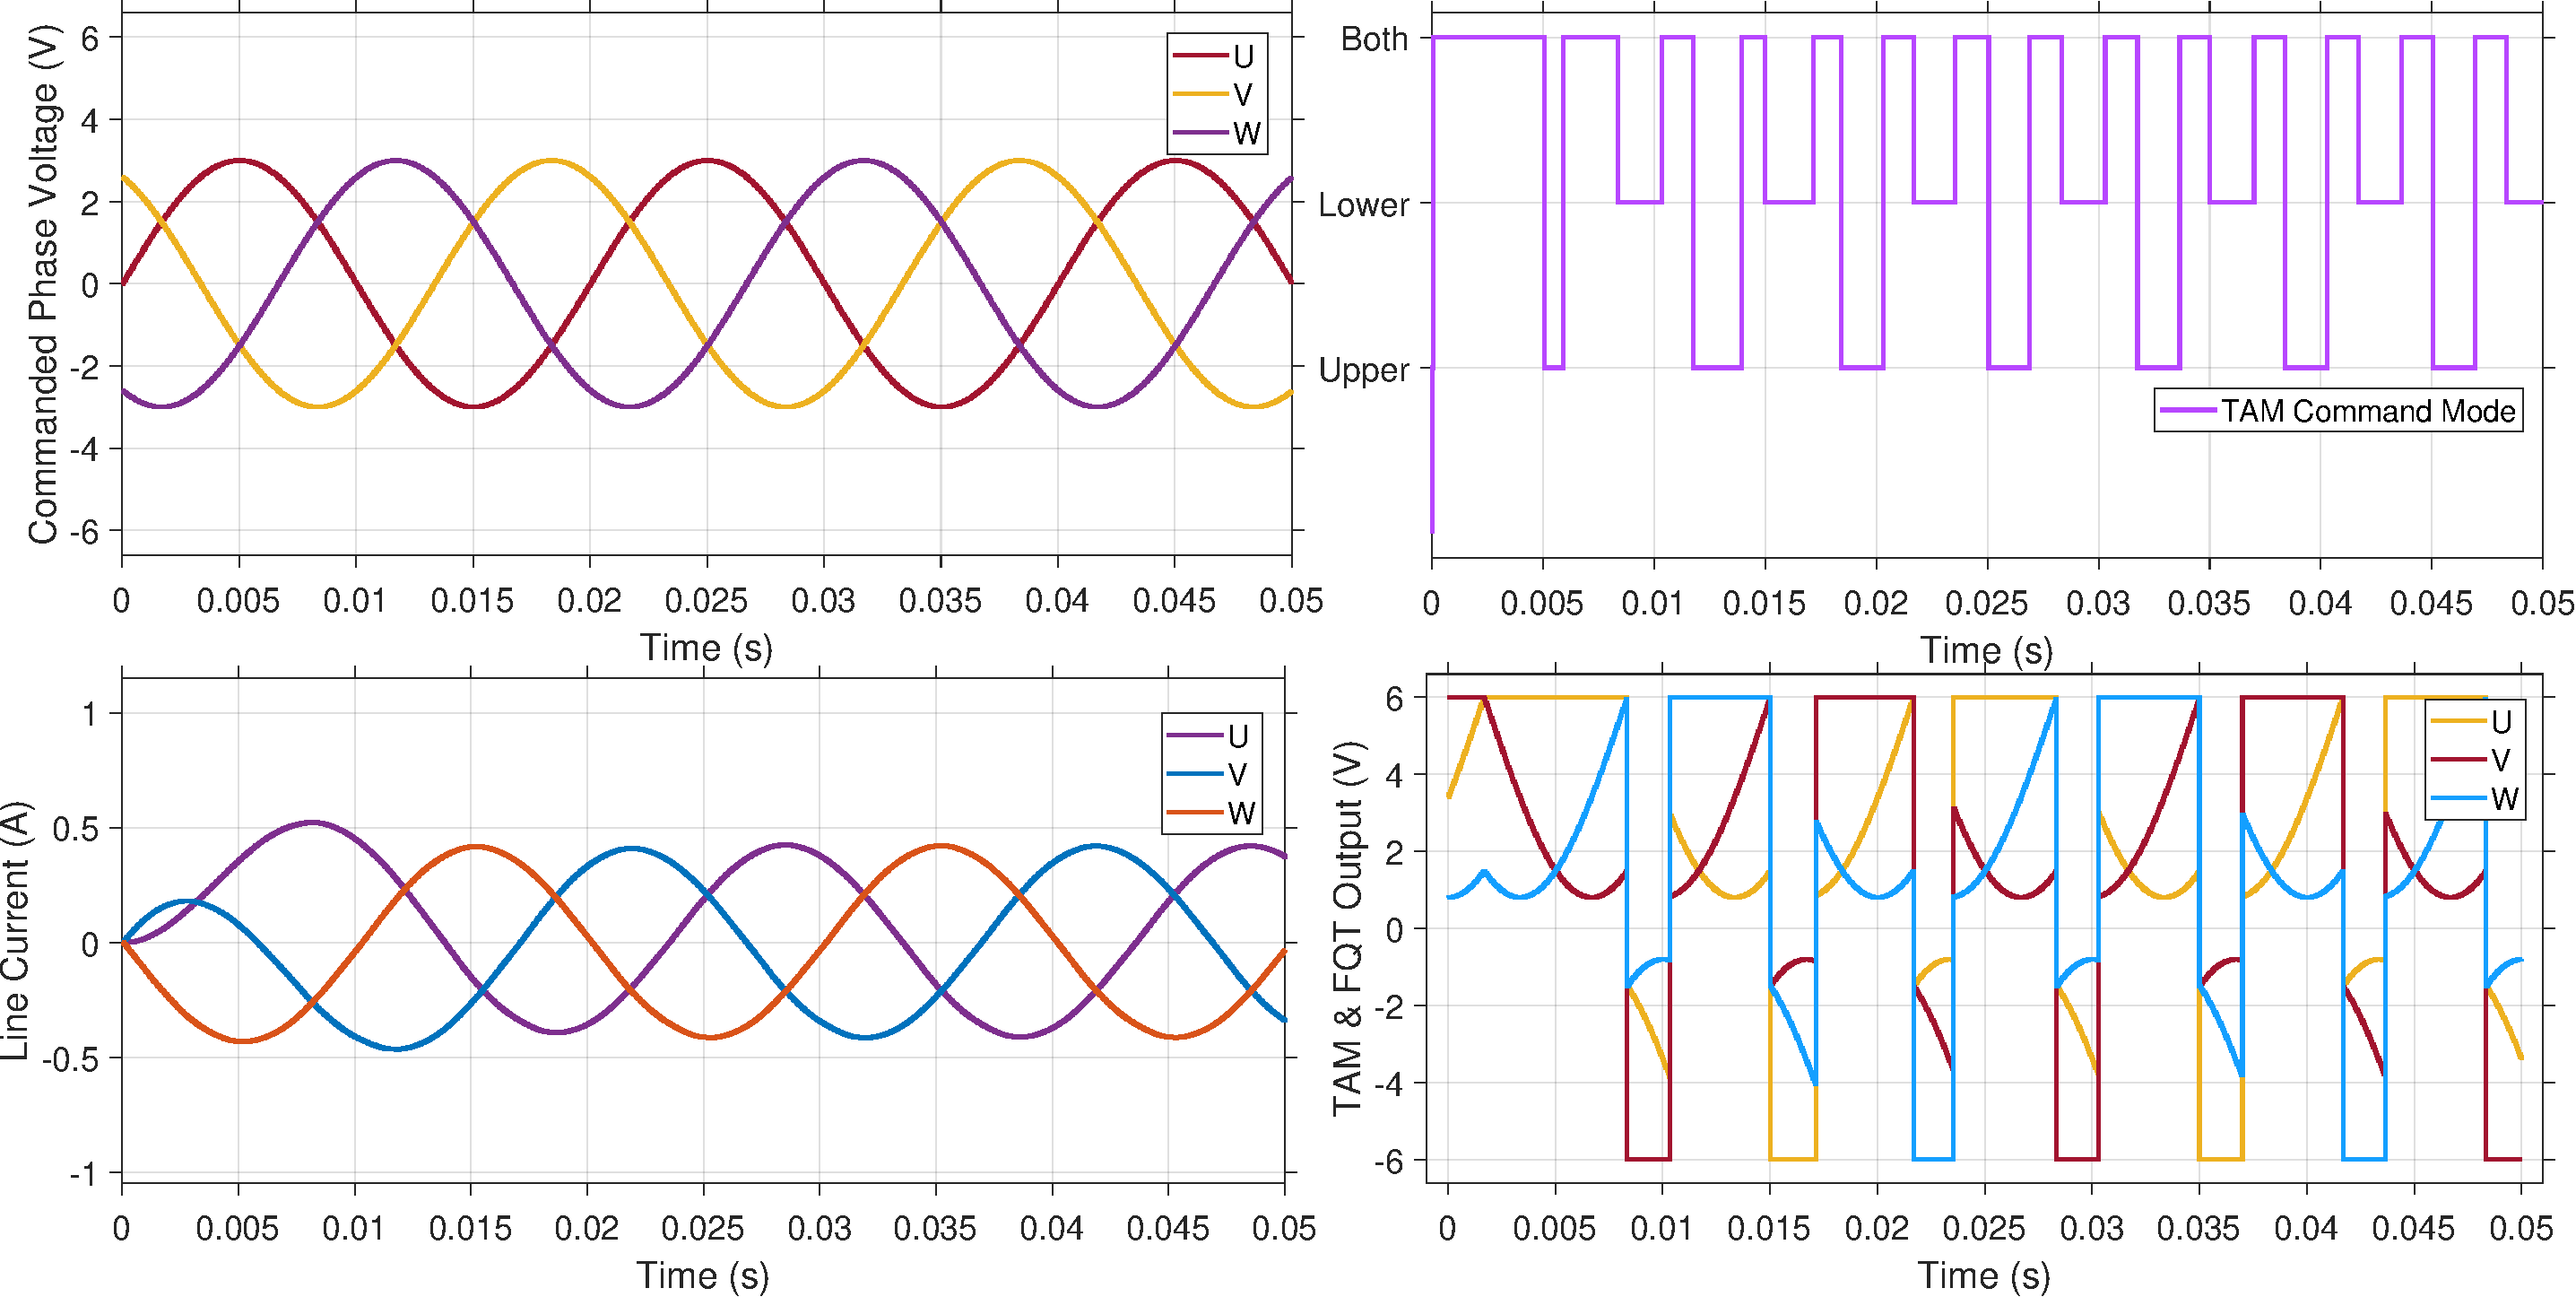
\includegraphics[width=\textwidth]{3V.pdf}
    \caption{ผลการทดลองของระบบอินเวอร์เตอร์ที่ปรับขนาดของค่ายอดของดันเฟสคำสั่งเท่ากับ 3 V}
    \label{3V}
\end{figure}

\begin{figure}[H]
    \centering
    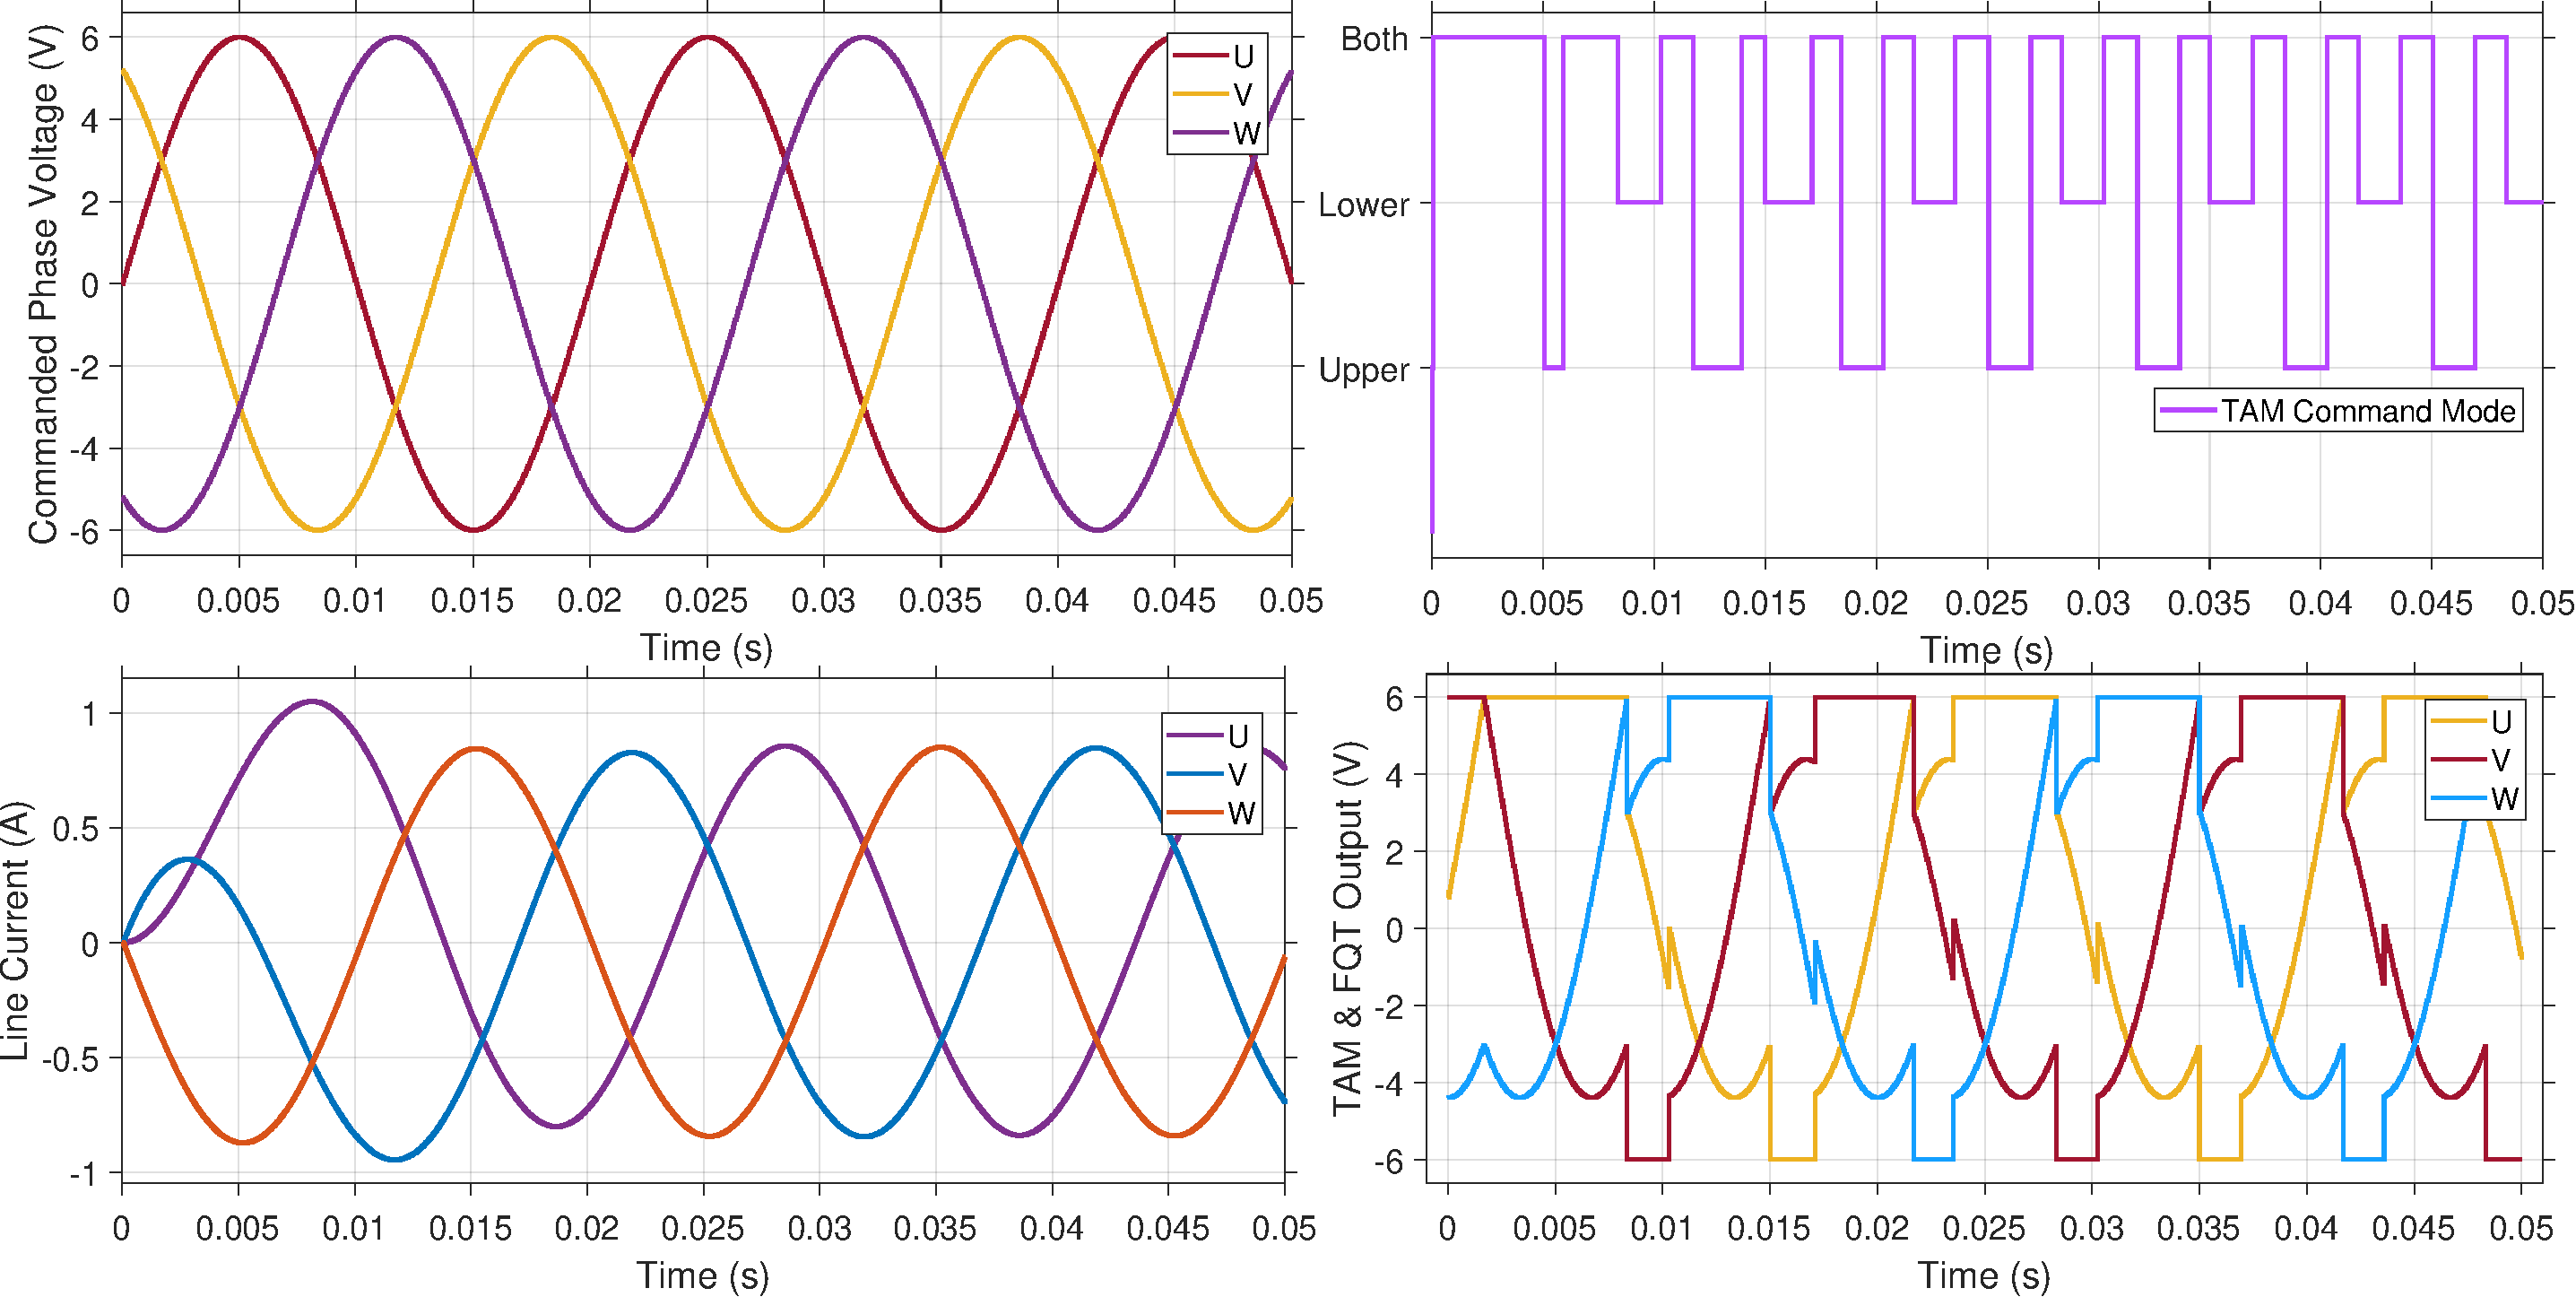
\includegraphics[width=\textwidth]{6V.pdf}
    \caption{ผลการทดลองของระบบอินเวอร์เตอร์ที่ปรับขนาดของค่ายอดของดันเฟสคำสั่งเท่ากับ 6 V}
    \label{6V}
\end{figure}





\subsection{วงจรสมมูลทางไฟฟ้าที่รวมระบบทางกลของแผ่นพื้นเก็บพลังงานและเครื่องจักรไฟฟ้าซิงโครนัสชนิดแม่เหล็กถาวร}
จากการศึกษาการทำงานของทำงานของแผ่นพื้นเก็บพลังงาน และ การเปรียบเทียบเชิงกล - ไฟฟ้า(Electrical analogy) เพื่อแปลงระบบทางกลของแผ่นพื้นเก็บพลังงานเป็นวงจรสมมูลทางไฟฟ้า มีขั้นตอนดังนี้

เนื่องจากอัตราส่วนของเกียร์ของ ขบวนเฟือง(gear train) และเฟืองดอกจอก(bevel gear) ที่ใช้ในการส่งการเคลื่อนที่เชิงหมุนจากเกลียวนำ(lead screw) ไปยังโรเตอร์ของเครื่องกำเนิดไฟฟ้าซิงโครนัส มีอัตราส่วนเท่ากับ 1:1 จึงได้ความสัมพันธ์
\begin{equation}\label{linear2angular}
    x = \frac{l\theta_{1}}{2\pi} = \frac{l\theta_{2}}{2\pi}
\end{equation}
จากสมการที่ (18)-(20) จะพิจารณจากแนวการเคลื่อนที่เชิงเส้นไปยังการเคลื่อนที่เชิงหมุนโดยใช้ความสัมพันธ์จากสมการที่ (\ref{linear2angular}) และใช้ความสัมพันธ์ของปริมาณทางกลและไฟฟ้าจากตารางที่ 1
\begin{equation}
    \frac{aml}{2\pi}\ddot{\theta}_{1} + \frac{aDl}{2\pi}\dot{\theta}_{1} + \frac{akl}{2\pi}\theta_{1} + aF_{a} = aF_(t)
\end{equation}
\begin{equation}
    J_{1}\ddot{\theta}_{1} + T_{B} = aF_{a}
\end{equation}
\begin{equation}
    J_{G}\ddot{\theta}_{2} + T_{G} = T_{B}
\end{equation}
\begin{figure}[!htb]
    \begin{center}
        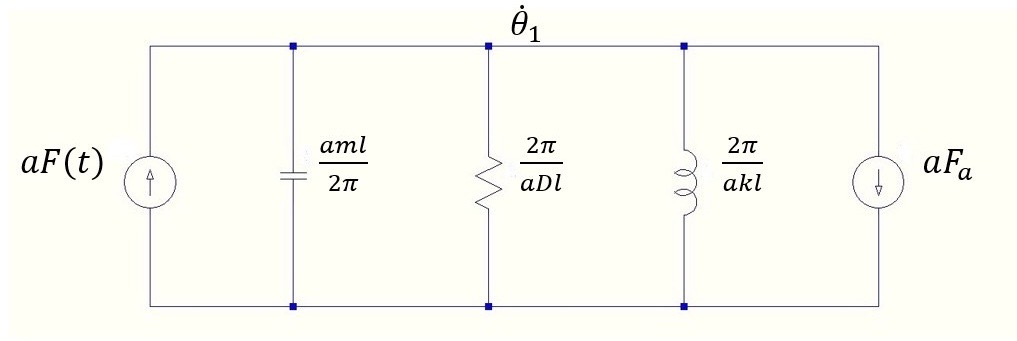
\includegraphics[width=0.7\textwidth]{cir1lx.jpeg}
    \end{center}
    \caption{วงจรไฟฟ้าของการเลื่อนที่ของแป้นเกลียว(nut)}
    \label{cir1lx}
\end{figure}
\begin{figure}[!htb]
    \begin{center}
        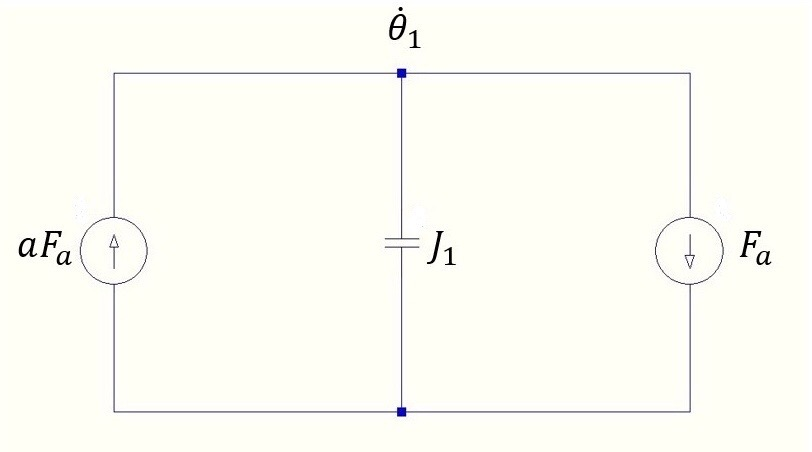
\includegraphics[width=0.5\textwidth]{cir2lx.jpg}
    \end{center}
    \caption{วงจรไฟฟ้าของการเคลื่อนที่เชิงหมุนของเกลียวนำ(lead screw)}
    \label{cir2_lx}
\end{figure}
\begin{figure}[H]
    \begin{center}
        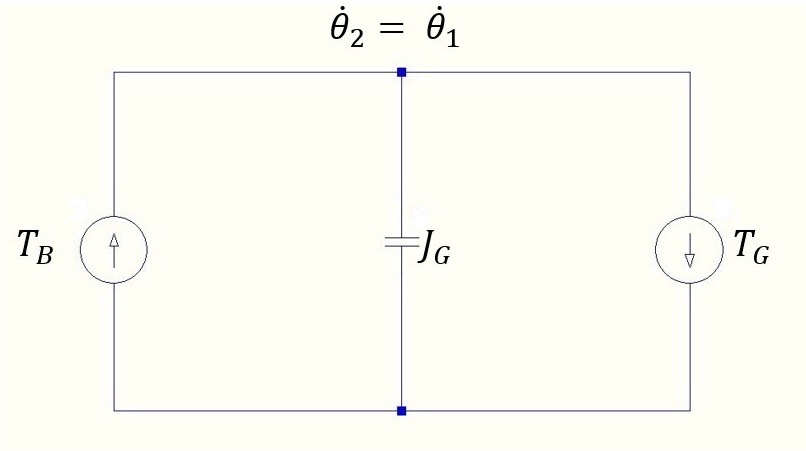
\includegraphics[width=0.5\textwidth]{cir3lx.jpg}
    \end{center}
    \caption{วงจรไฟฟ้าของโรเตอร์ของเครื่องกำเนิดไฟฟ้า}
    \label{cir3lx}
\end{figure}
จากรวมวงจรไฟฟ้าของการเลื่อนที่ของแป้นเกลียว(nut) และ การเคลื่อนที่เชิงหมุนของเกลียวนำ(lead screw) และ โรเตอร์ของเครื่องกำเนิดไฟฟ้า ทั้งสามข้างบน จะได้ วงจรสมมูลทางไฟฟ้าระบบทางกลของแผ่นพื้นเก็บพลังงาน ดังรูปที่ \ref{cir4lx}

\begin{figure}[H]
    \begin{center}
        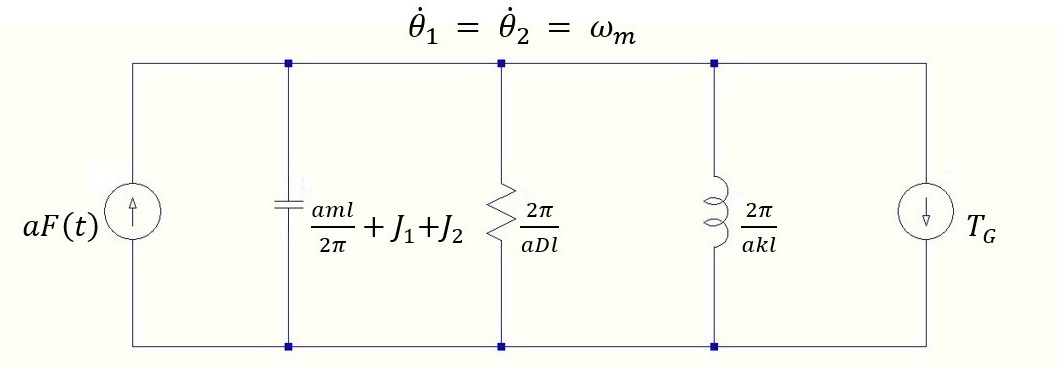
\includegraphics[width=0.7\textwidth]{cir4lx.jpg}
    \end{center}
    \caption{วงจรสมมูลไฟฟ้าของระบบทางกลของแผ่นพื้นเก็บพลังงาน}
    \label{cir4lx}
\end{figure}

หลังจากได้วงจรสมมูลทางไฟฟ้าของระบบทางกลของแผ่นพื้นเก็บพลังงาน จึงได้ศึกษาเครื่องจักรกลไฟฟ้าซิงโครนัสชนิดแม่เหล็กถาวรเพื่อเข้าใจหลักกรทำงานและสมการความสัมพันธ์ต่างๆ ที่จะสามารถวิเคราะห์ และสร้างวงจรสมมูลไฟฟ้าที่รวมระบบทางกลของแผ่นพื้นเก็บพลังงานและเครื่องจักรไฟฟ้าซิงโครนัสชนิดแม่เหล็กถาวร

จากการที่ได้ศึกษาเครื่องจักรไฟฟ้าซิงโครนัสชนิดแม่เหล็กถาวร และได้วงจรมูลของระบบทางกลของแผ่นพื้นเก็บพลังงาน สามารถรวมระบบทางกลของแผ่นพื้นเก็บพลังงานและเครื่องจักรไฟฟ้าซิงโครนัสชนิดแม่เหล็กถาวรตามขั้นตอน ดังนี้

จากสมการถที่ (17) แรงดันบนกรอบอ้างอิงนิ่ง แกน x,y ทำให้ทราบความสัมพันธ์ของแรงเคลื่อนเหนี่ยวนำภายในของเครื่องจักรไฟฟ้าซิงโครนัสชนิดแม่เหล็กถาวร ดังสมการด้านล่าง

\begin{equation}
    e_{x} = p \lambda \omega_{m} cos(\theta_{e})
\end{equation}
\begin{equation}
    e_{x} = p \lambda \omega_{m} sin(\theta_{e})
\end{equation}
\begin{equation}
    \vec{e}_{ind} =
    \begin{bmatrix}
        e_{x} \\ e_{y}
    \end{bmatrix} = E
    \begin{bmatrix}
        cos(\theta_{e}) \\ sin(\theta_{e})
    \end{bmatrix} = p \lambda \omega_{m}
    \begin{bmatrix}
        cos(\theta_{e}) \\ sin(\theta_{e})
    \end{bmatrix} =
    p \lambda e^{j\theta_{e}}
\end{equation}

วงจรที่ไฟฟ้าของระบบทางกลของแผ่นพื้นเก็บพลังงานสัมพันธ์กับเครื่องจักรไฟฟ้าซิงโครนัสชนิดแม่เหล็กถาวรผ่านหม้อแปลงไฟฟ้า ความเร็วของโรเตอร์สะท้อนไปยังขนาดแรงเคลื่อนเหนี่ยวของเครื่องจักรไฟฟ้าซิงโครนัสตามสมการด้านบน จึงได้ความสัมพันธ์แสดงดังรูปวงจรด้านล่าง
\begin{figure}[H]
    \begin{center}
        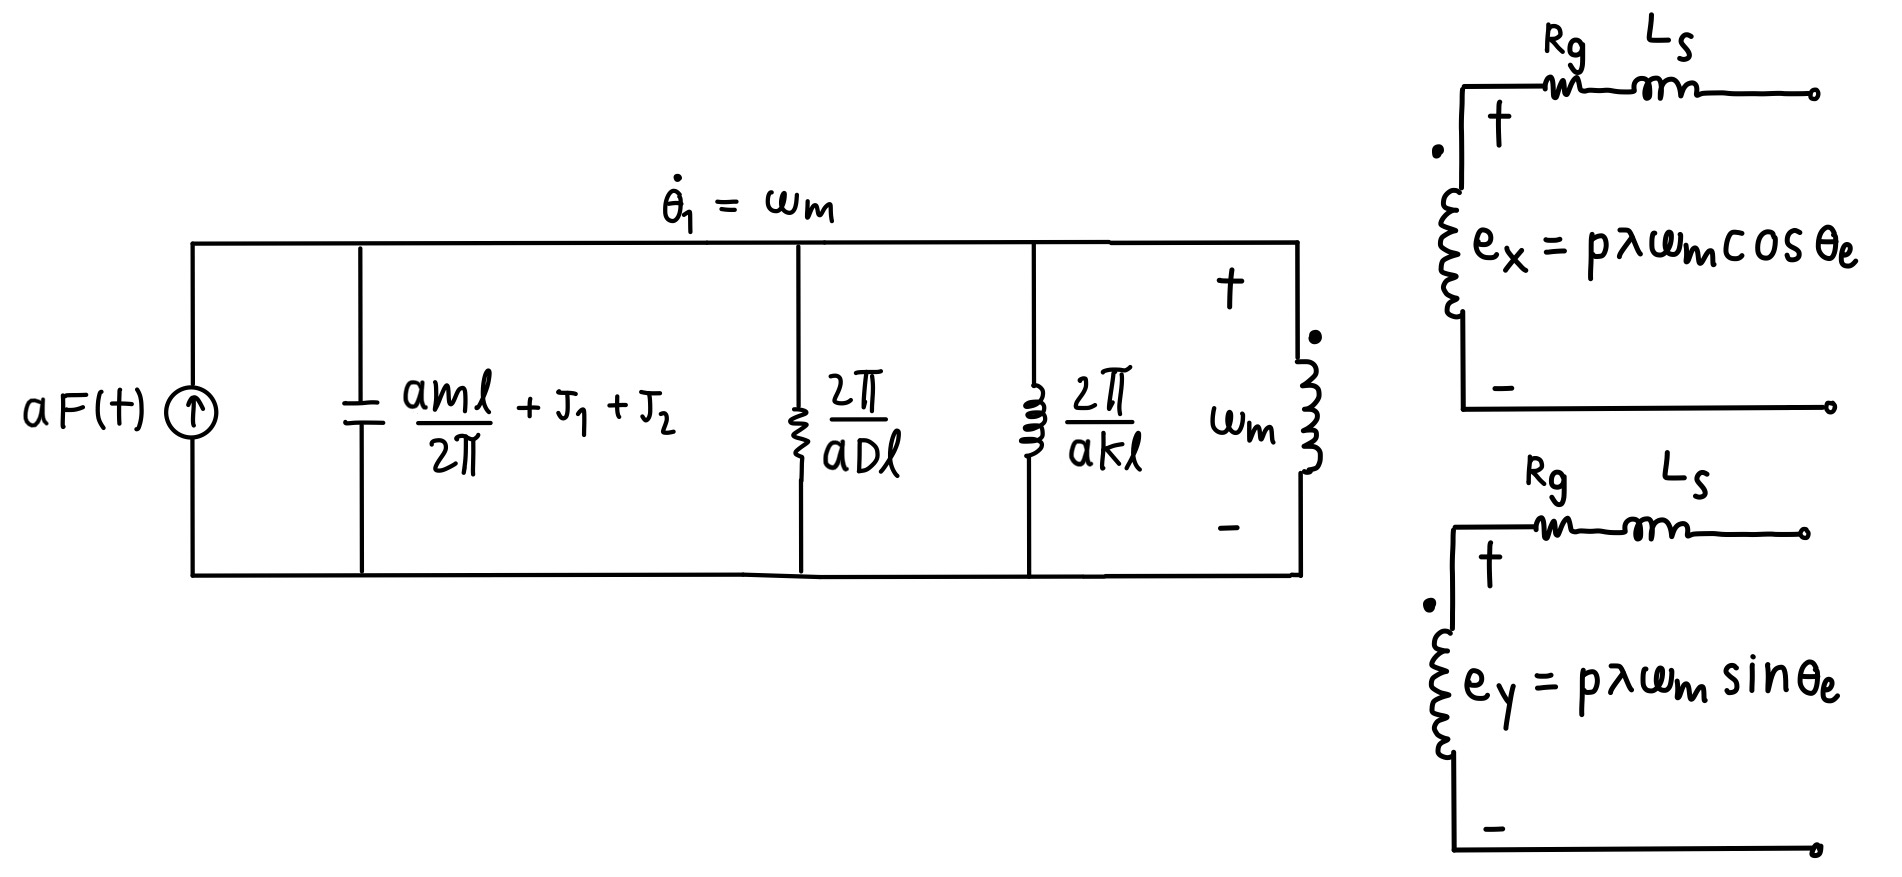
\includegraphics[width=0.8\textwidth]{cir_mech_elec_1n.jpg}
    \end{center}
    \caption{วงจรไฟฟ้าแสดงความสัมพันธ์ระบบทางกลและเครื่องกำเนิดไฟฟ้า}
    \label{cir_mech_elec_1n}
\end{figure}

จากนั้นเขียนความสัมพันธ์อยู่ในรูปสเปซเวกเตอร์ของระบบทางกลของแผ่นพื้นเก็บพลังงานและ เครื่องจักรไฟฟ้าซิงโครนัสชนิดแม่เหล็กถาวร เพื่อสามารถวิเคราะห์เป็นวงจรไฟฟ้าเพียงวงจรเดียวได้
\begin{equation}
    \begin{bmatrix}
        e_{x} \\ e_{y}
    \end{bmatrix} = p\lambda
    \begin{bmatrix}
        cos(\theta_{e}) & -sin(\theta_{e}) \\ sin(\theta_{e}) & cos(\theta_{e})
    \end{bmatrix}
    \begin{bmatrix}
        \omega_{m} \\ 0
    \end{bmatrix}
\end{equation}
\begin{equation}
    \begin{bmatrix}
        e_{x} \\ e_{y}
    \end{bmatrix} = p\lambda e^{-J \theta_{e} }
    \begin{bmatrix}
        \omega_{m} \\ 0
    \end{bmatrix}
\end{equation}

จึงสามารถมองเป็นวงจรสมมูลที่แสดงความสัมพันธ์เป็นหม้อแปลงไฟฟ้าที่มีอัตราส่วนจำนวนรอบเป็นเชิงซ้อน ดังรูปที่ \ref{cir_mech_elec2n2}
\begin{figure}[H]
    \begin{center}
        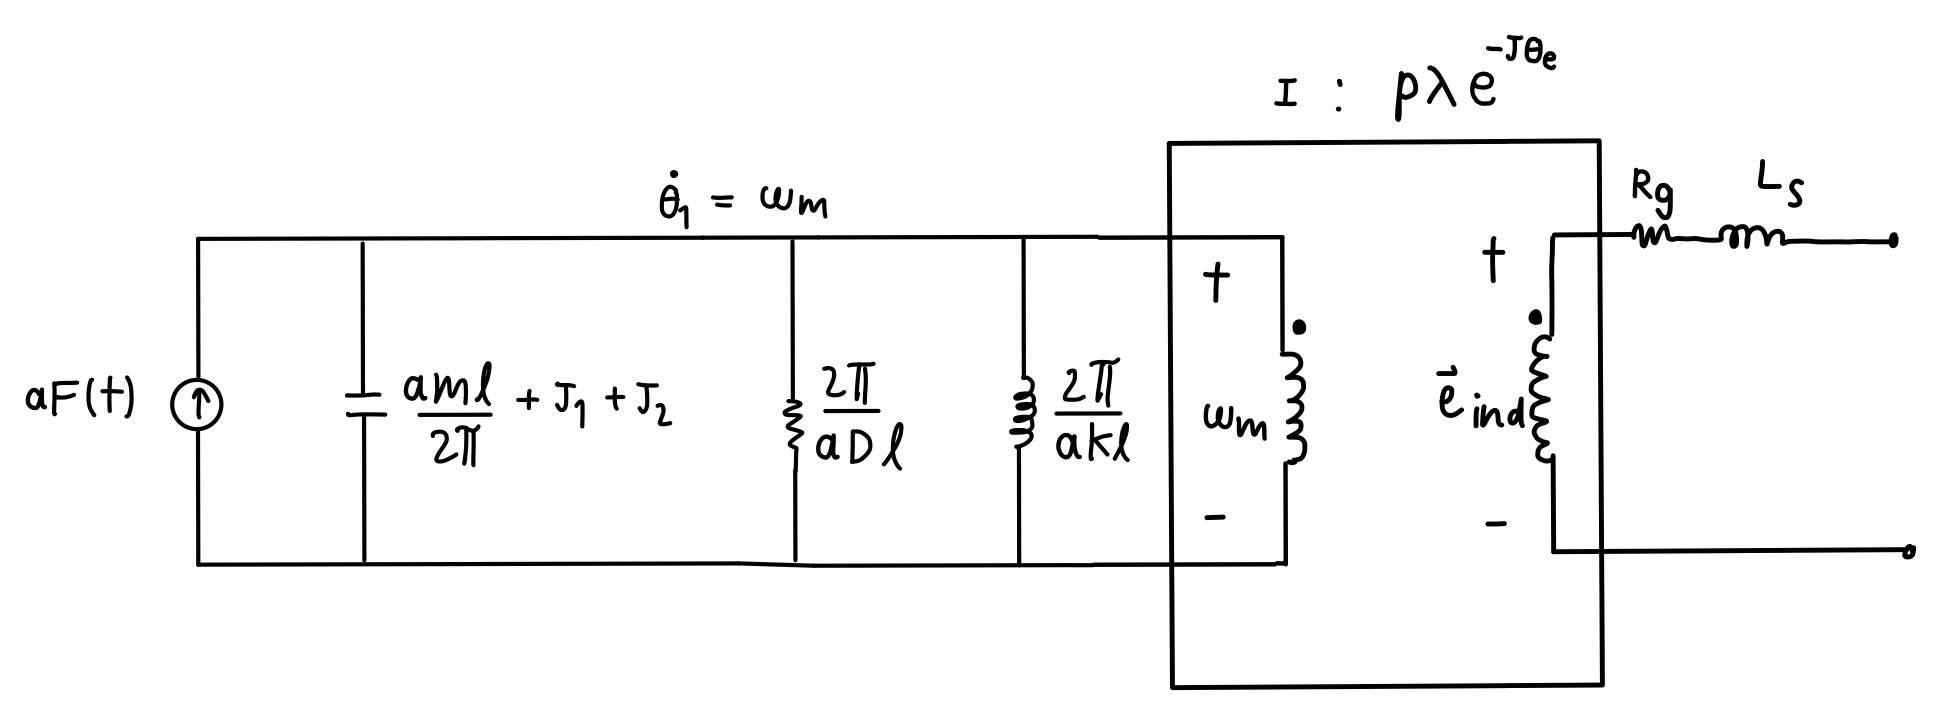
\includegraphics[width=0.8\textwidth]{cir_mech_elec2n2.jpg}
    \end{center}
    \caption{วงจรไฟฟ้าแสดงความสัมพันธ์ระบบทางกลและเครื่องกำเนิดไฟฟ้าที่มีหม้อแปลงไฟฟ้ามีอัตราส่วนเป็นเชิงซ้อน}
    \label{cir_mech_elec2n2}
\end{figure}

จากนั้นทำการแปลงเป็นวงจรสมมูล โดยอ้างอิงฝั่งทุติยภูมิ(บน)และอ้างอิงฝั่งปฐมภูมิ(ล่าง) แสดงดังรูปที่ \ref{cir_mech_elec_3}
\begin{figure}[H]
    \begin{center}
        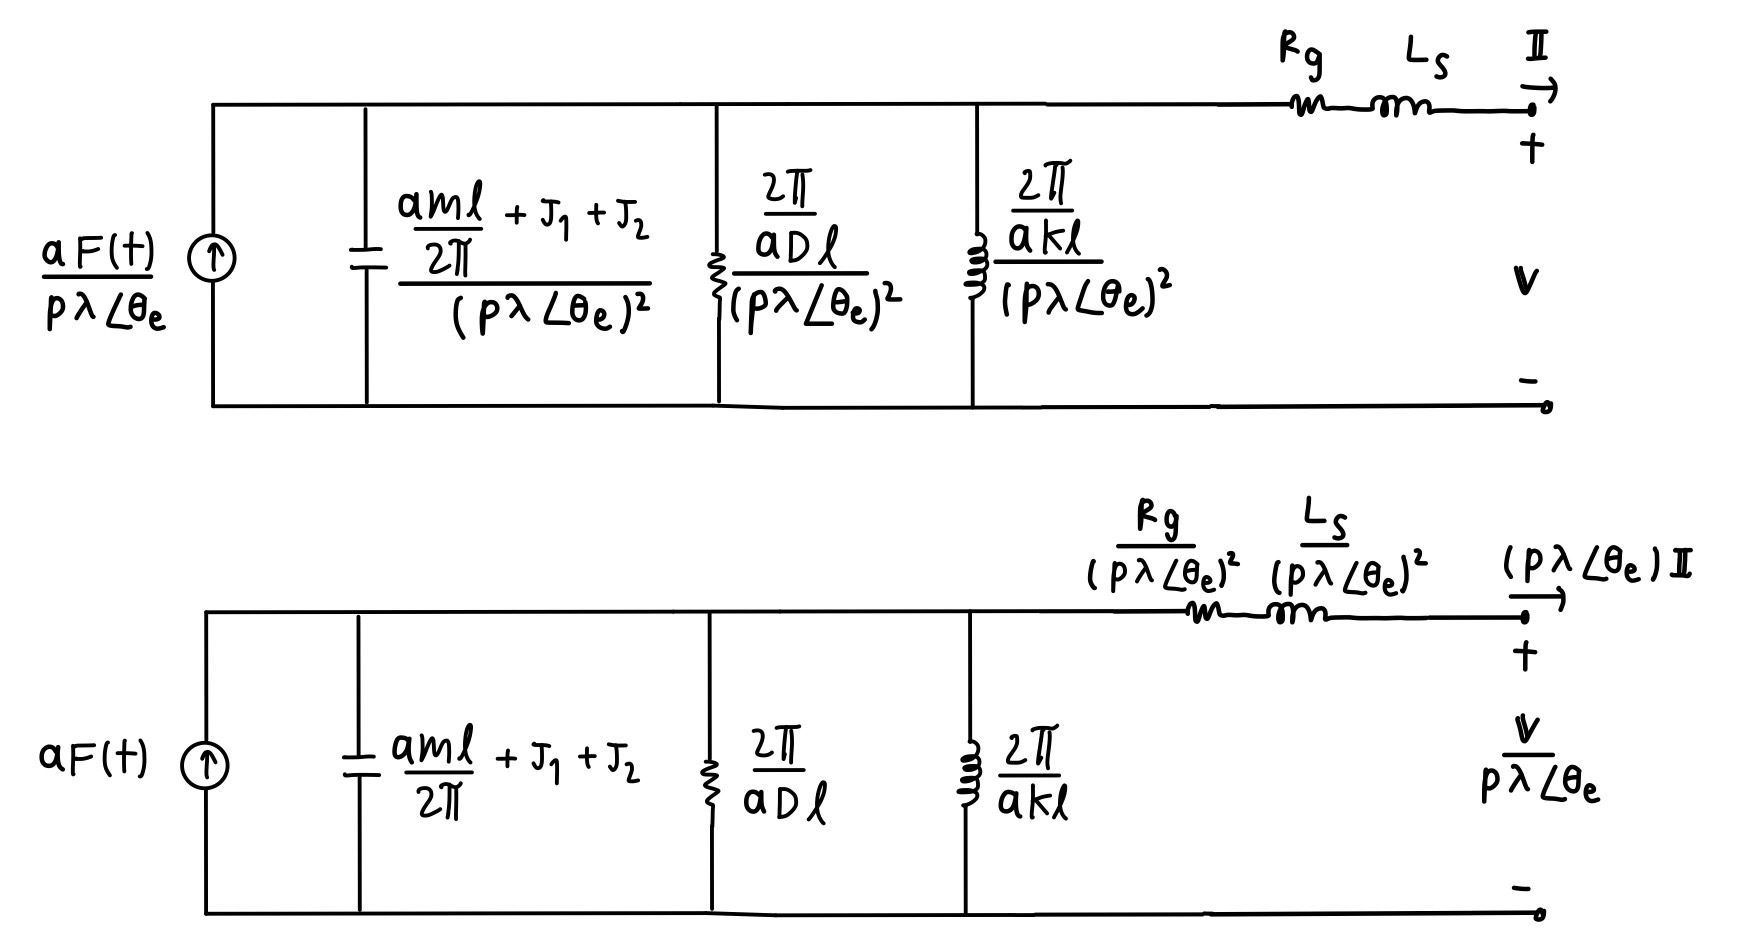
\includegraphics[width=0.8\textwidth]{cir_mech_elec_3.jpg}
    \end{center}
    \caption{วงจรสมมูลไฟฟ้าที่อ้างอิงฝั่งทุติยภูมิ(บน)และอ้างอิงฝั่งปฐมภูมิ(ล่าง)}
    \label{cir_mech_elec_3}
\end{figure}

\subsection{ผลการจำลองของแบบจำลองทางไฟฟ้าที่รวมระบบทางกลของแผ่นพื้นเก็บพลังงานและเครื่องจักรไฟฟ้าซิงโครนัสชนิดแม่เหล็กไฟฟ้า บนโปรแกรม MATLAB/Simulink}

จากสมการที่ (\ref{vter}) จึงทำการแปลงวงจรสมมูลจากรูป \ref{cir_mech_elec_3} โดยใช้ทฤษฎีเทเวนิน จะได้วงจรสมมูลดังรูปด้านล่าง
\begin{figure}[H]
    \begin{center}
        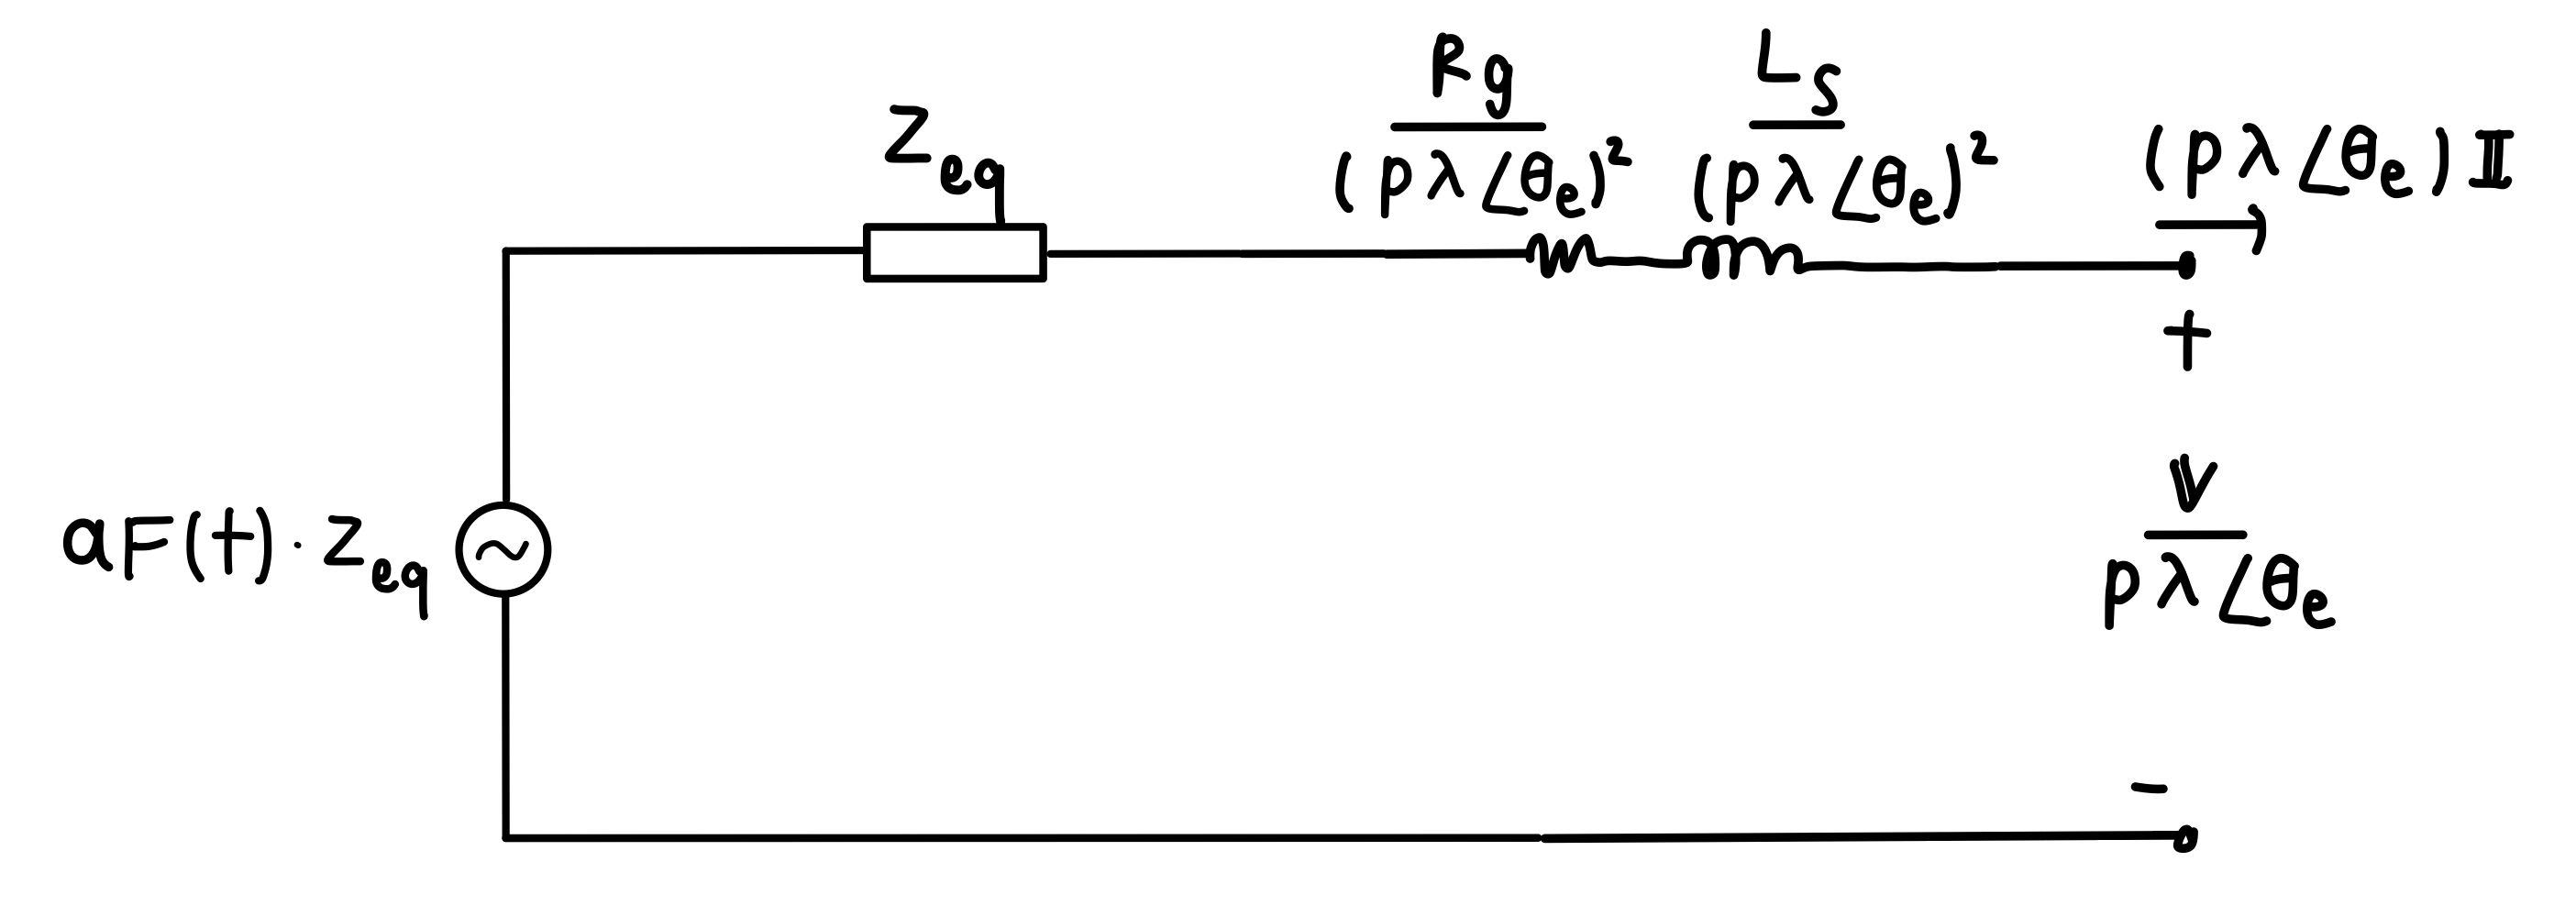
\includegraphics[width=0.7\textwidth]{cir_mech_elec_4.jpg}
    \end{center}
    \caption{แบบจำลองวงจรไฟฟ้าที่รวมระบบทางกลของแผ่นพื้นพลังงานและเครื่องกำเนิดไฟฟ้า โดยใช้ทฤษฎีเทเวนิน}
    \label{cir_mech_elec_4}
\end{figure}
โดย $Z_{eq}$ คือ $ \frac{2\pi}{aDl} // s \frac{2\pi }{akl} // \frac{1}{s( \frac{aml}{2\pi} + J_{1} + J_{2} ) }   $
จากทฤษฎีการถ่ายโอนกำลังสูงสุด จะได้ว่าโหลดที่นำมาต่อที่ด้านขาออกของเครื่องจักรไฟฟ้าซิงโครนัส จะมีลักษณะตามสมการที่ (\ref{zmppt})
\begin{equation}\label{zmppt}
    z_{load} = conjugate[ z_{eq} (p\lambda \angle \theta_{e})^2 + R_{g} + sL_{s} ]
\end{equation}
โดยแรงดันขาออกที่สอดคล้องกับหลักการติดตามจุดทำงาน ซึ่งทำให้กำลังขาออกของเครื่องจักรไฟฟ้ามีค่าสูงสุดเป็นดังสมการที่ (\ref{vmppt})
\begin{equation}\label{vmppt}
    v_{out} = conjugate[ z_{eq} I (p\lambda \angle \theta_{e})^2 + R_{g}I + sL_{s}I ]
\end{equation}

หลังจากที่ได้วงจรสมมูลไฟฟ้าที่รวมระบบทางกลของแผ่นพื้นเก็บพลังงานและเครื่องจักรไฟฟ้าซิงโครนัสและเงื่อนไขแรงดันขาออกที่สอดคล้องกับหลักการติดตามจุดทำงานซึ่งทำให้กำลังขาออกมีค่าสูงสุด จากรูปที่ \ref{cir_mech_elec_4} และสมการต่างๆที่เกี่ยวข้อง มาสร้างแบบจำลองบนโปรแกรม MATLAB/Simulink ดังรูปที่ \ref{sim_elecmech} เพื่อศึกษาการทำงานของแบบจำลองที่ได้

\begin{figure}[H]
    \begin{center}
        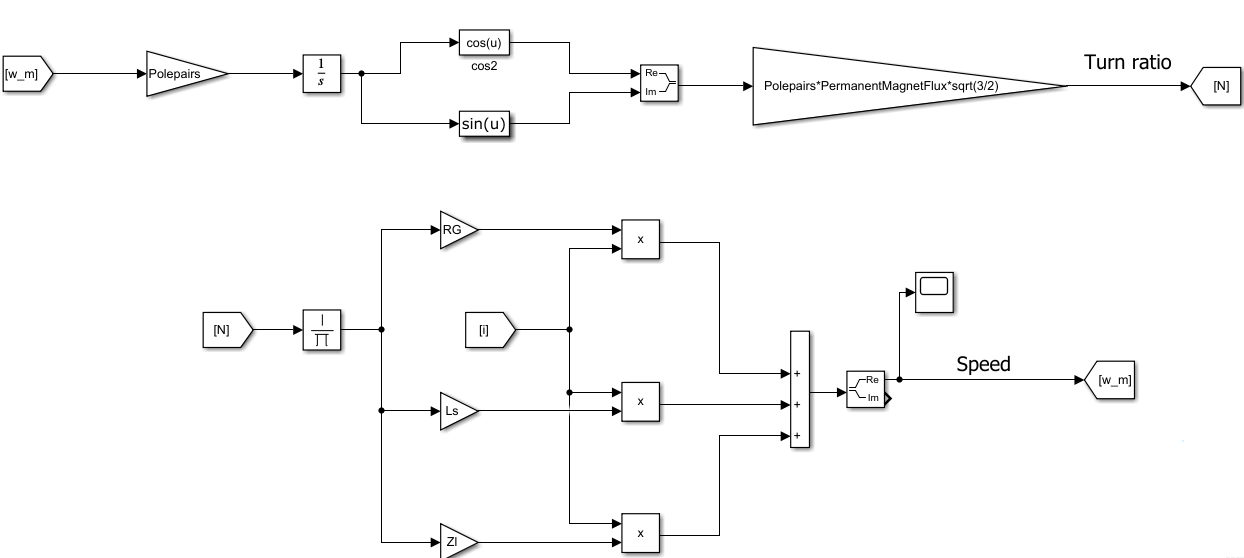
\includegraphics[width=0.8\textwidth]{sim_elecmech_2.png}
        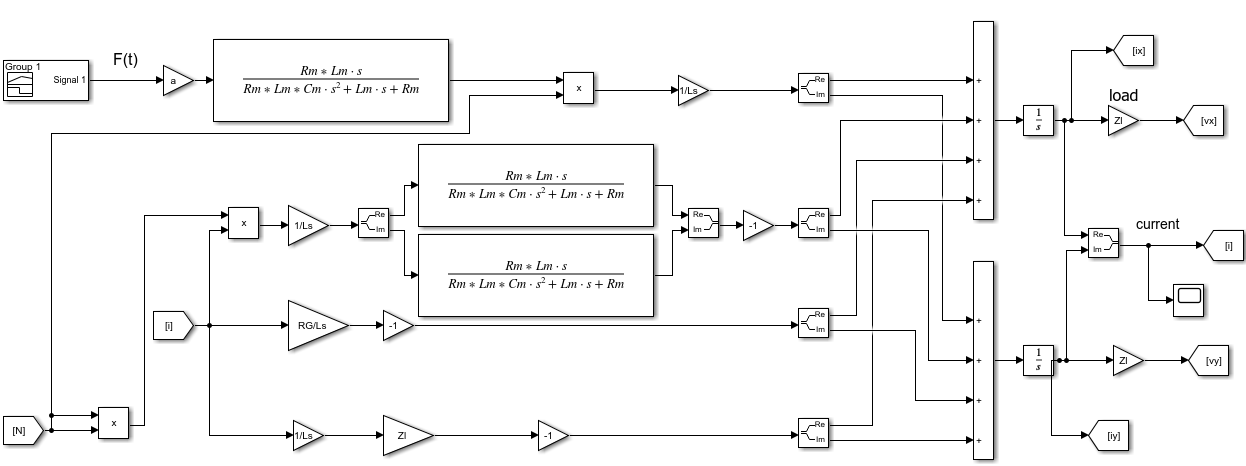
\includegraphics[width=1\textwidth]{sim_elecmech_3.png}
    \end{center}
    \caption{แบบจำลองวงจรสมมูลไฟฟ้าที่รวมระบบทางกลของแผ่นพื้นพลังงานและเครื่องกำเนิดไฟฟ้า ที่มีโหลดตัวต้านทาน 32.23 โอห์ม}
    \label{sim_elecmech}
\end{figure}

แบบจำลองที่ได้ ทดสอบด้วยแรงเหยียบ ดังรูปที่ \ref{sim_elecmech} และใส่โหลดเป็นตัวต้านทานที่ขาออกของ มีขนาดเท่ากับความต้านทานภายในเครื่องจักรไฟฟ้าซิงโครนัสชนิดแม่เหล็กไฟฟ้า ซึ่งมีค่าเท่ากับ 32.23 โอห์ม ใช้แรงจากเท้าเหยียบแสดงดังรูปที่ \ref{force_sim} ค่าพารามิเตอร์อื่นที่ใช้ในการทดสอบ \cite{GpH:01} แสดงดังตารางที่ \ref{mech_param} และ \ref{pmsm_param}
\begin{figure}[H]
    \begin{center}
        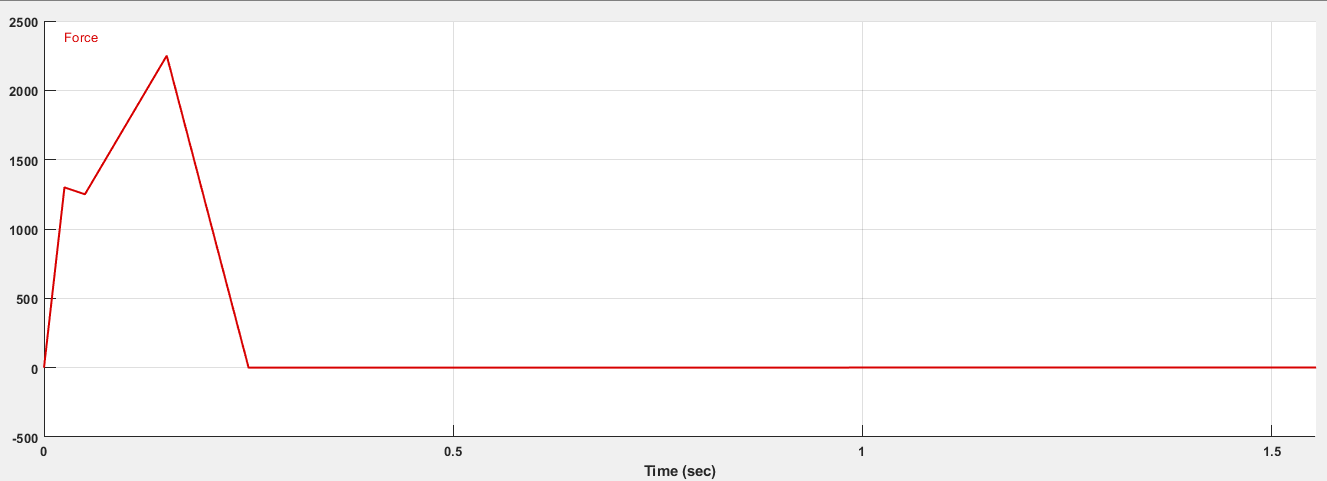
\includegraphics[width=0.8\textwidth]{force_sim.png}
    \end{center}
    \caption{แบบจำลองวงจรสมมูลไฟฟ้าที่รวมระบบทางกลของแผ่นพื้นพลังงานและเครื่องกำเนิดไฟฟ้า ที่มีโหลดตัวต้านทาน 32.23 โอห์ม}
    \label{force_sim}
\end{figure}

\begin{table}
    \centering
    \begin{tabular}{ | l | l | l | p{5cm} |}
        \hline
        \textbf{Parameters}                      & \textbf{Value}           \\ \hline
        Pitch of lead screw                      & 8 mm                     \\ \hline
        lead(l)                                  & 0.015 m                  \\ \hline
        Mass of nut and plate(m)                 & 2.16 kg                  \\ \hline
        Moment of inertia of bevel gear($J_{G}$) & 8.6756 x $10^-7$ kg$m^2$ \\ \hline
        Moment of inertia of lead screw($J_{l}$) & 2.5536 x $10^-6$ kg$m^2$ \\ \hline
        lead angle                               & 45 degree                \\ \hline
        Spring coefficient(k)                    & 40000 N/m                \\ \hline
        Damping coefficient(D)                   & 2000 Ns/m                \\ \hline
        Friction coefficient($\mu$)              & 0.21                     \\ \hline
        Efficient of thrust bearing              & 1.00                     \\ \hline
        Efficient of thread                      & 0.8                      \\ \hline
    \end{tabular}
    \caption{ค่าตัวแปรทางกลที่เกี่ยวข้องกับแผ่นพื้นพลังงาน \cite{GpH:01}}
    \label{mech_param}
\end{table}

\begin{table}
    \centering
    \begin{tabular}{ | l | l | l | p{5cm} |}
        \hline
        \textbf{Parameters}                              & \textbf{Value} \\ \hline
        ค่าความต้านทานของขดลวดสเตเตอร์(Rs)                  & 32.23 $\Omega$ \\ \hline
        ค่าความเหนี่ยวนำของขดลวดสเตเตอร์(Ls)                 & 11.3 mH        \\ \hline
        ค่าความเหนี่ยวนำของขดลวดสเตเตอร์ในแนวแกนอ้างอิงดี (Ld)  & 16 mH          \\ \hline
        ค่าความเหนี่ยวนำของขดลวดสเตเตอร์ในแนวแกนอ้างอิงคิว (Lq) & 16 mH          \\ \hline
        ฟลักซ์แม่เหล็กของแม่เหล็กถาวร                          & 0.009 Wb       \\ \hline
        จำนวนคู่ขั้ว                                         & 6 คู่            \\ \hline
    \end{tabular}
    \caption{ค่าตัวแปรทางกลที่เกี่ยวข้องกับเครื่องจักรไฟฟ้าซิงโครนัสแม่เหล็กถาวร\cite{GpH:01}}
    \label{pmsm_param}
\end{table}



\begin{figure}[H]
    \begin{center}
        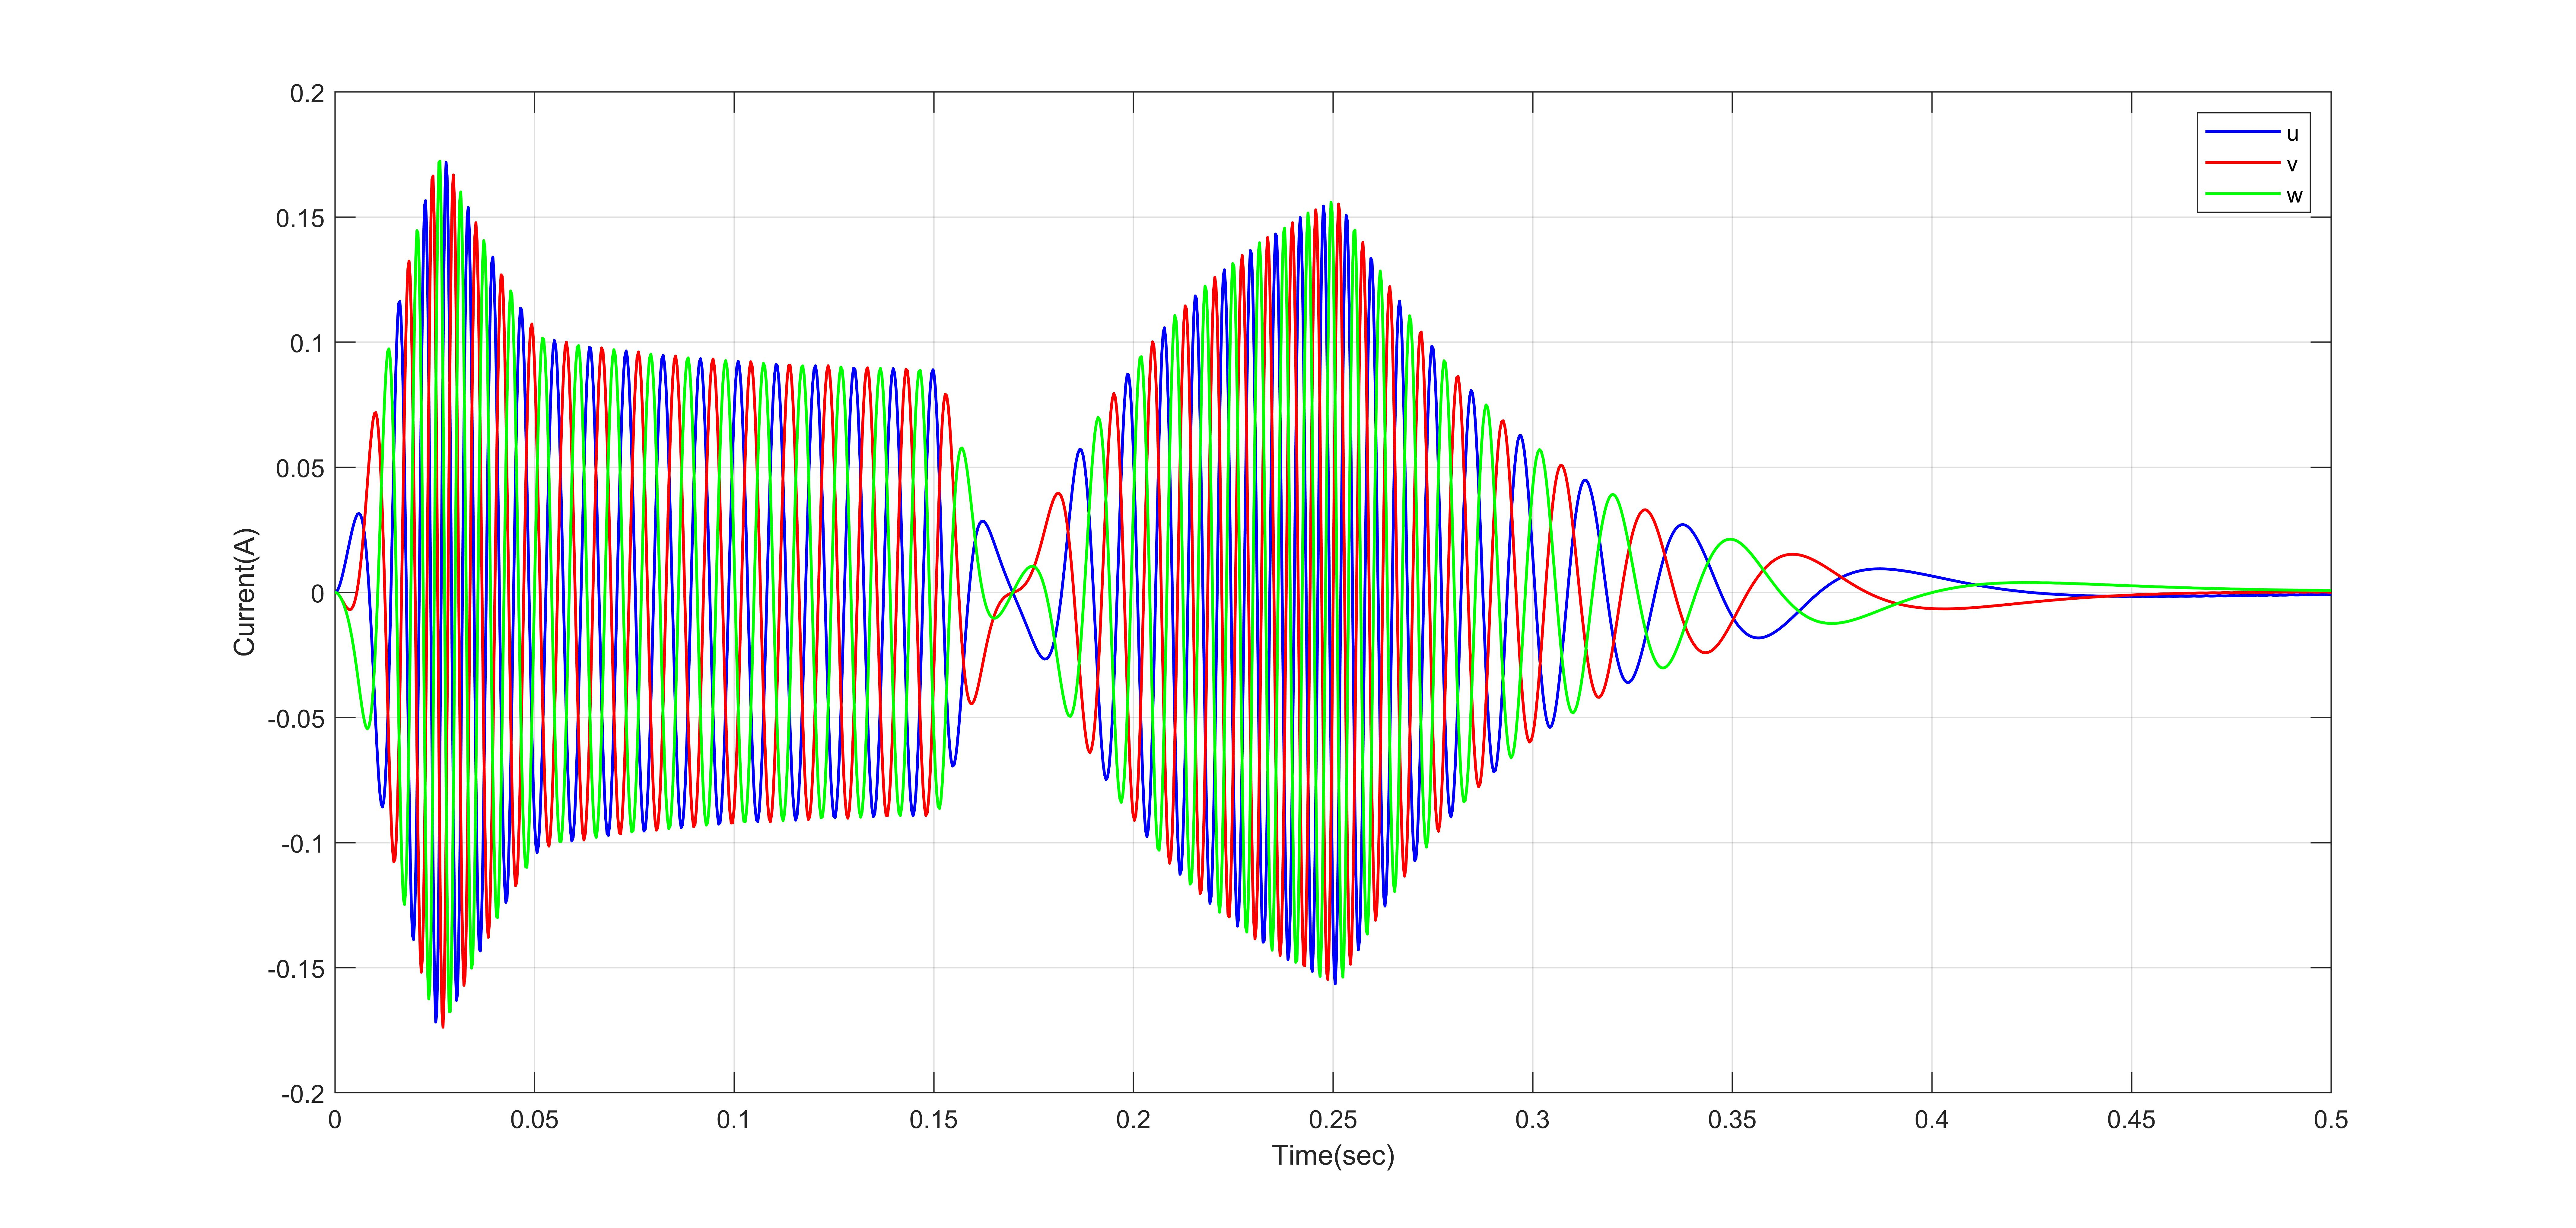
\includegraphics[width=1\textwidth]{current_1.jpg}
    \end{center}
    \caption{กระแสขาออก เมื่อโหลดตัวต้านทาน 32.23 โอห์ม}
    \label{current_1}
\end{figure}
\begin{figure}[H]
    \begin{center}
        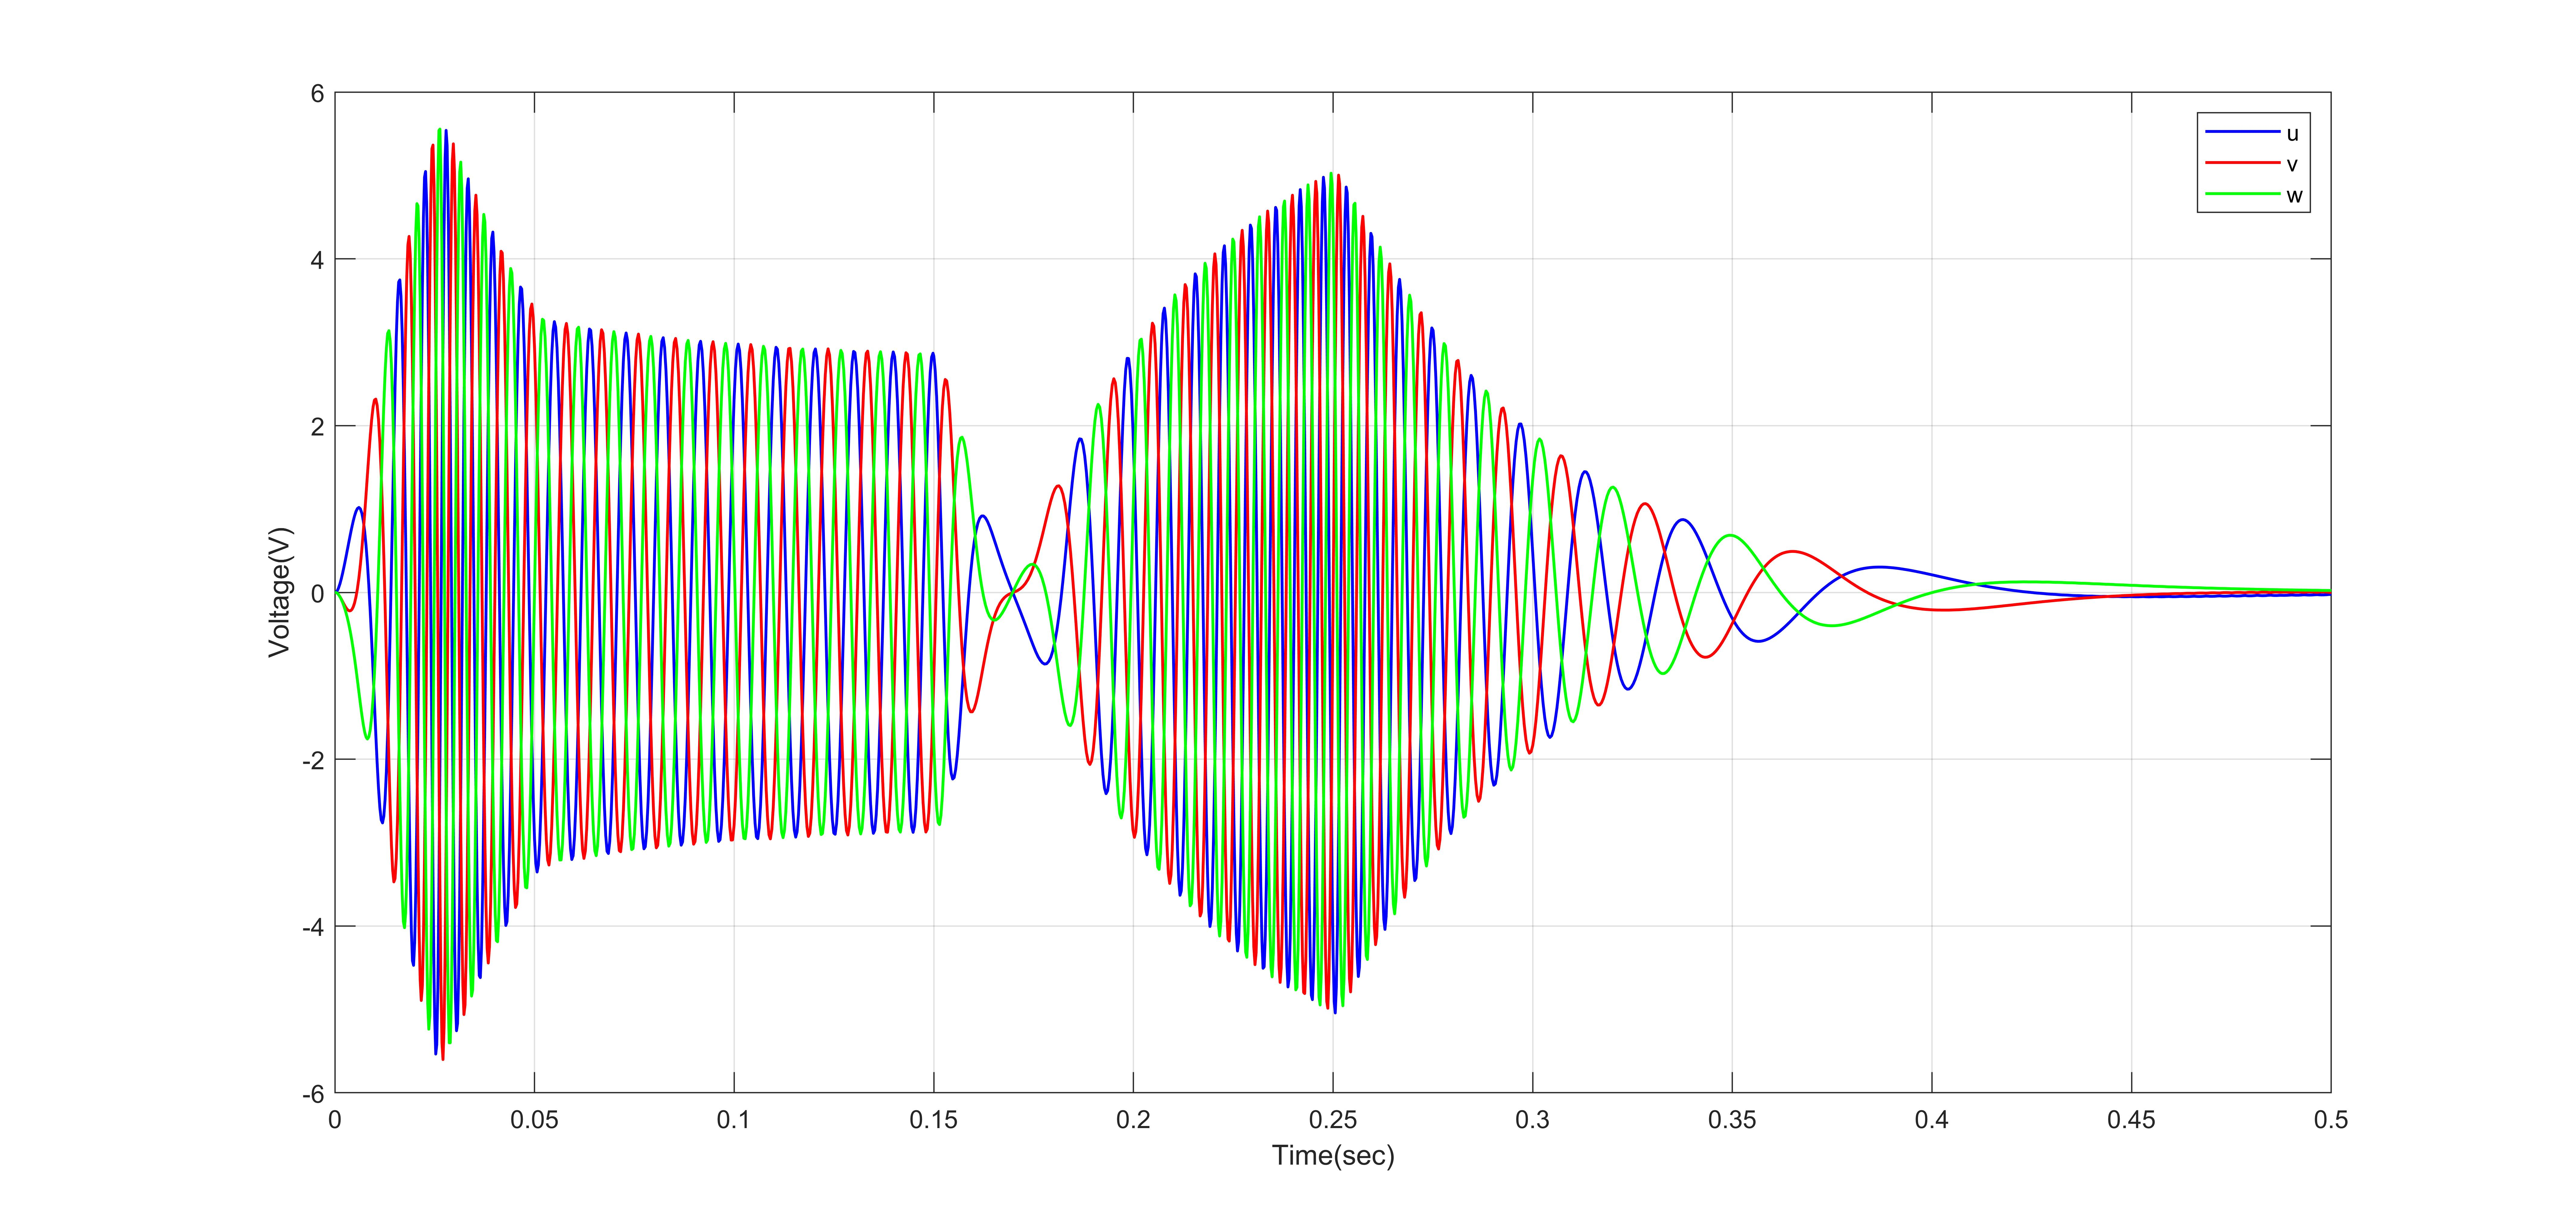
\includegraphics[width=1\textwidth]{voltage_1.jpg}
    \end{center}
    \caption{แรงดันขาออก เมื่อโหลดตัวต้านทาน 32.23 โอห์ม}
    \label{voltage_1}
\end{figure}


จากรูปที่ \ref{current_1} และ \ref{voltage_1} พบว่า แรงดันและกระแสมีลูกคลื่นเกิดขึ้นจำนวน 2 ลูก โดยลูกแรกเกิดจากการยุบตัวของแผ่นพื้นเนื่องจากแรงที่เหยียบลงบนแผ่นพื้นเก็บพลังงาน และลูกที่สองเกิดจากการยุบตัวของแผ่นพื้นเนื่องจากแรงคืนตัวของสปริง

จากสมการที่ (\ref{vter}) เมื่อเปลี่ยนโหลดจากตัวต้านทานเป็นแหล่งจ่ายแรงดันแบบควบคุมได้ สามารถนำมาสร้างเป็นอัลกอริทึมการติดตามจุดทำงานสูงสุดได้ดังรูปที่ \ref{mppt_v}
โดยนำกระแสขาออกของแบบจำลองมาพิจารณาผ่านอัลกอริทึมการติดตามจุดทำงานสูงสุดเพื่อคำนวณหาเงื่อนไขสัญญาณแรงดันที่เหมาะสมและส่งกลับไปเป็นสัญญาณแรงดันขาออกของเครื่องจักรกลไฟฟ้าซิงโครนัส ซึ่งจะทำให้ได้กำลังขาออกสูงสุด
\begin{figure}[H]
    \begin{center}
        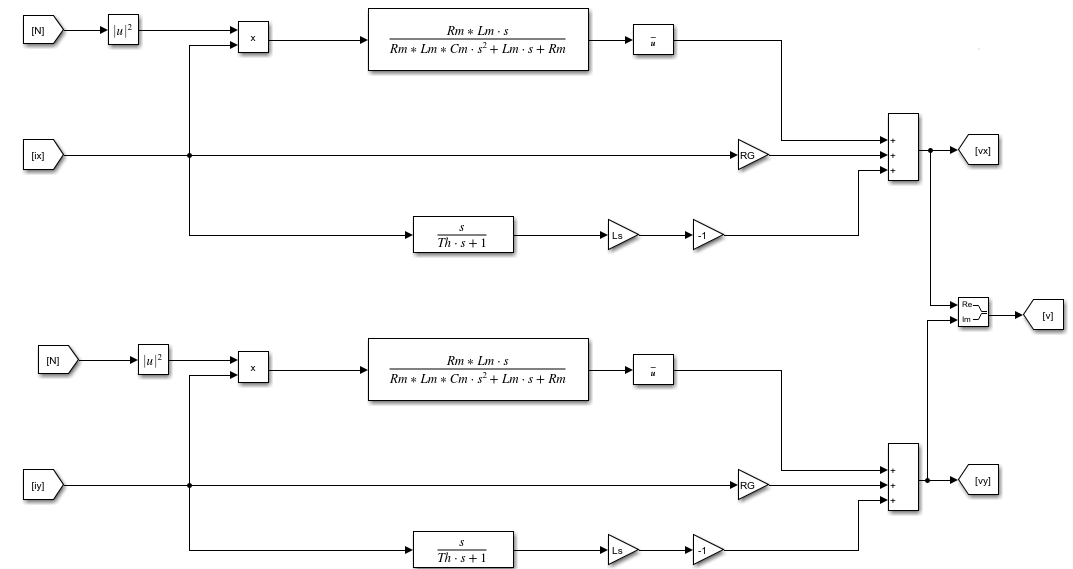
\includegraphics[width=1\textwidth]{mppt_v.png}
    \end{center}
    \caption{แผนภาพไดอะแกรมของอัลกอริทึมการติดตามจุดทำงานสูงสุดบนแกนอ้างอิงนิ่ง}
    \label{mppt_v}
\end{figure}

จากผลการทดสอบแบบจำลอง จะได้ว่ากำลังขาออกเมื่อมีการใช้อัลกอริทึมการติตามกำลังสูงสุด ที่มาจากวงจรสมมูลไฟฟ้าที่รวมระบบทางกลของแผ่นพื้นเก็บพลังงานและเครื่องจักรไฟฟ้าซิงโครนัสมีลักษณะดังรูปที่ \ref{mppt_graph}
และเปรียบเทียบกำลังขาออกเมื่อไม่มีการรวมระบบทางกลของแผ่นพื้นเก็บพลังงานมาคิดรวมในอัลกอริทึมการติดตามกำลังสูงสุดในปีการศึกษา 2563

\begin{figure}[H]
    \begin{center}
        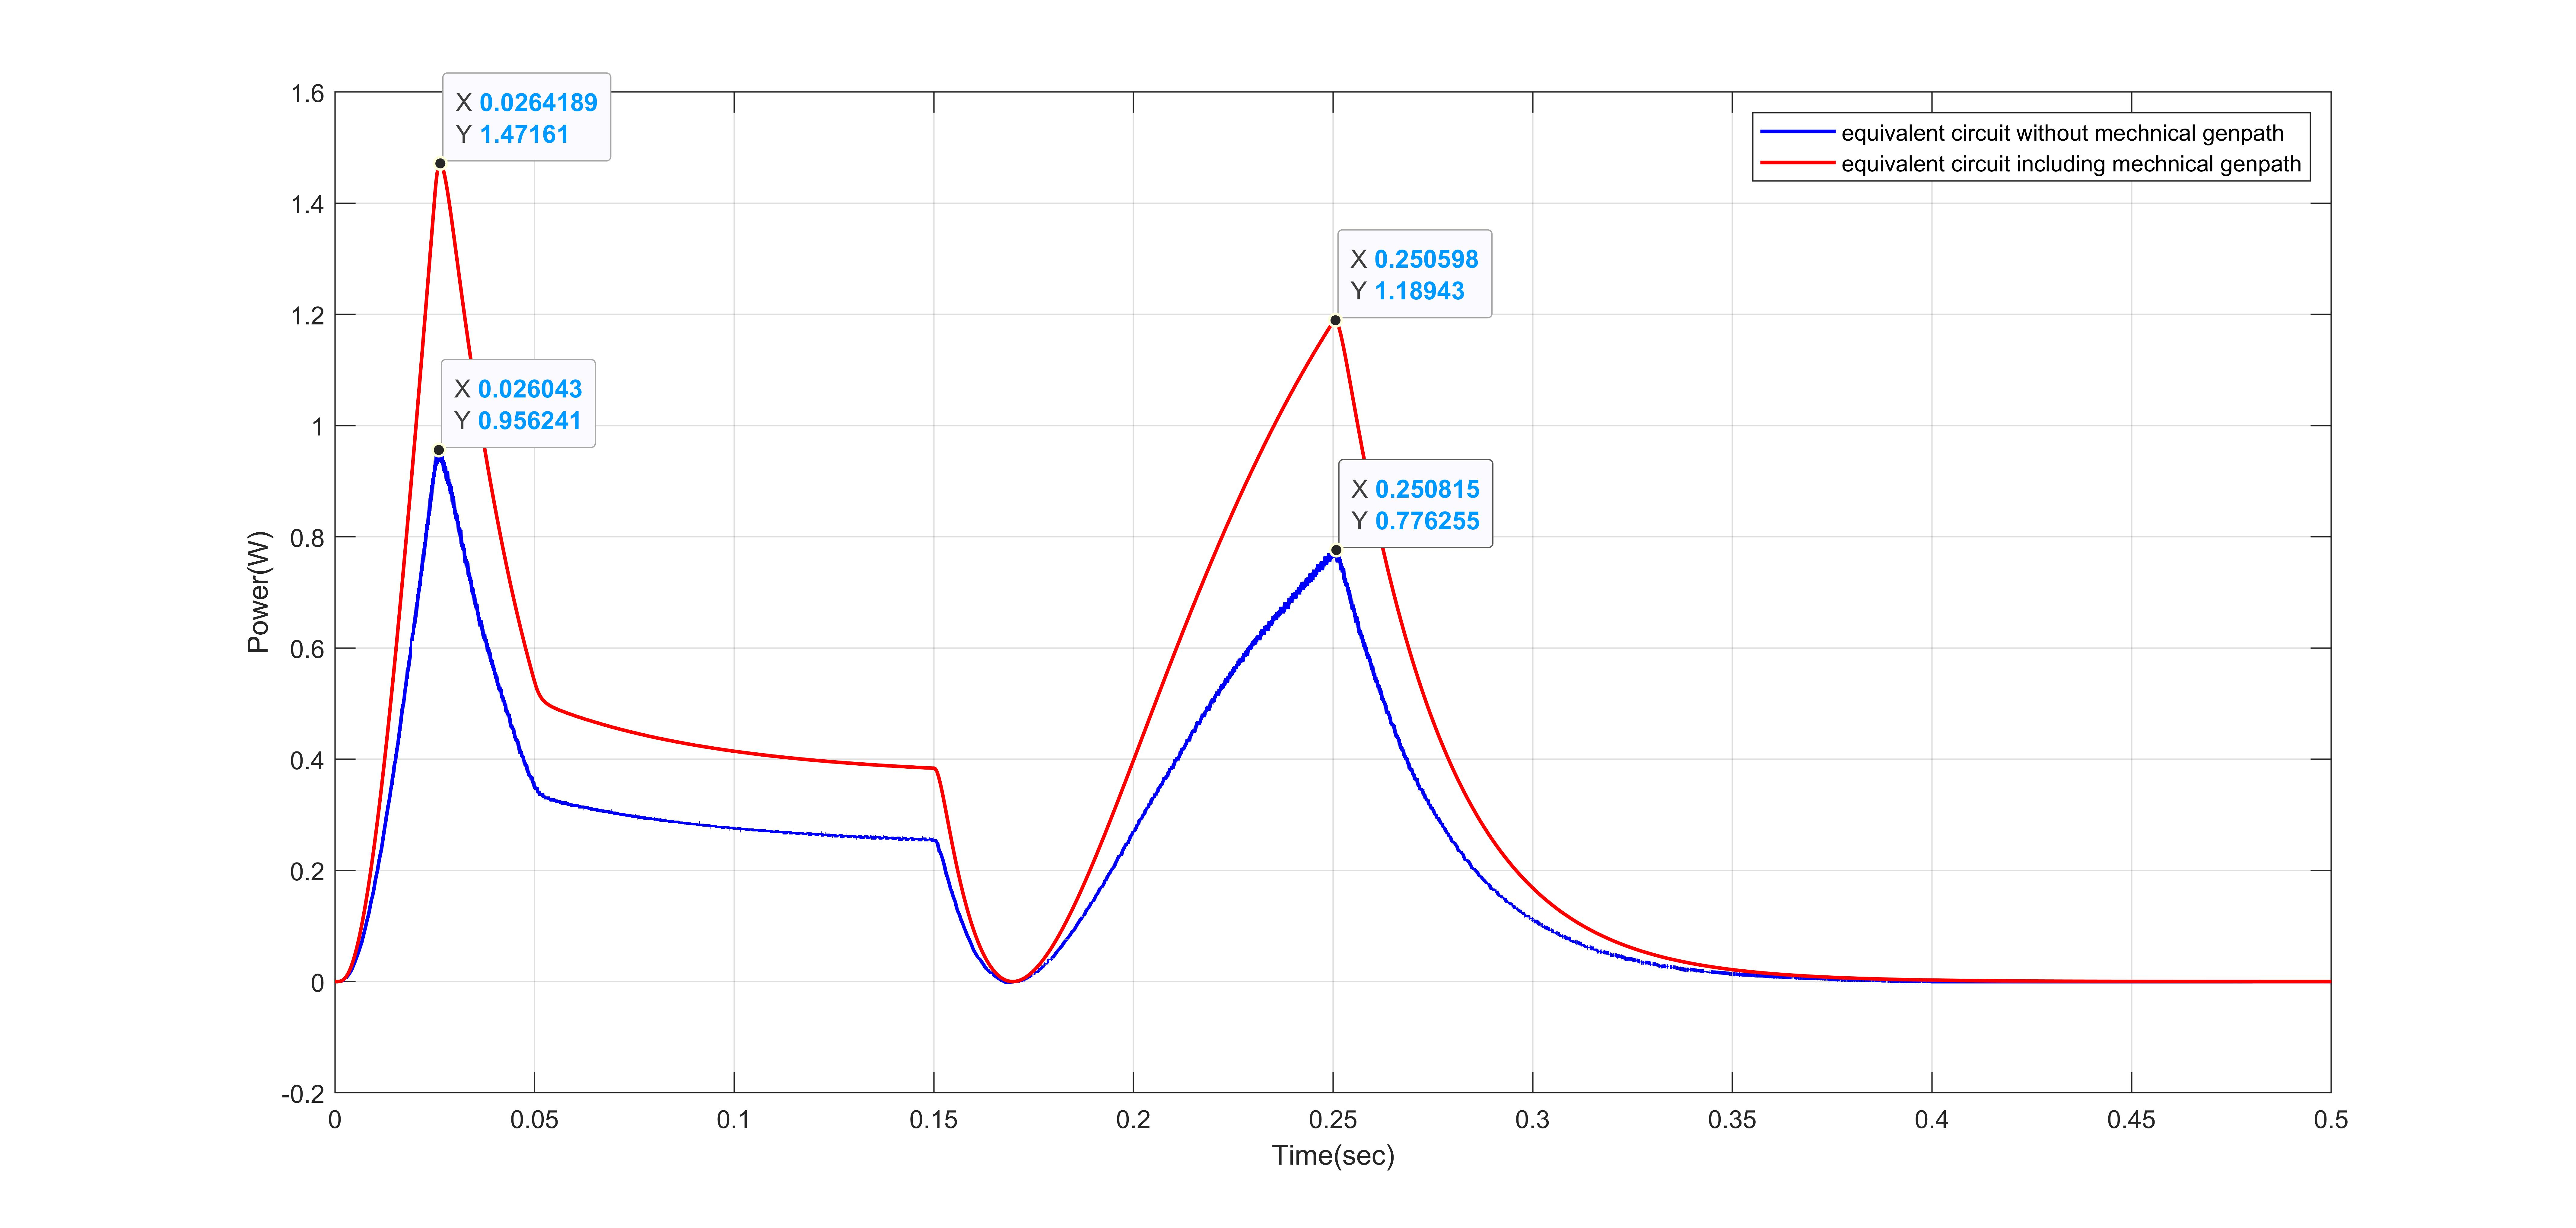
\includegraphics[width=1\textwidth]{mppt_graph.jpg}
    \end{center}
    \caption{กำลังขาออกเมื่ออัลกอริทึมการติดตามจุดทำงานสูงสุด กรณีที่รวมระบบทางกลของแผ่นพื้นเก็บพลังงานมาคำนวณ และกรณีที่ไม่รวมระบบทางกลของแผ่นพื้นเก็บพลังงานมาคำนวณ}
    \label{mppt_graph}
\end{figure}

จากรูป \ref{mppt_graph} พบว่ากรณีที่รวมระบบทางกลของแผ่นพื้นเก็บพลังงานมาคำนวณด้วย จะได้กำลังขาออกที่สูงกว่า กรณีที่ไม่รวมระบบทางกลของแผ่นพื้นเก็บพลังงานมาคำนวณ
กำลังขาออกสูงสุดค่ายอดลูกแรกเพิ่มจาก 0.95 วัตต์ เป็น 1.47 วัตต์ และกำลังขาออกสูงสุดค่ายอดลูกที่สองเพิ่มจาก 0.77 วัตต์ เป็น 1.18 วัตต์ จึงสรุปได้ อัลกอริทึมการติดตามจุดทำงานสูงสุด กรณีที่รวมระบบทางกลของแผ่นพื้นเก็บพลังงานมาคำนวณ สามารถทำให้ได้กำลังขาออกมีค่าที่สูงขึ้นจริง
เนืองจาก พิจารณาสมการ (\ref{zmppt}) และ (\ref{vmppt}) จะมีพจน์อิมพีแดนซ์ $Z_{eq}$ ซึ่งเท่ากับ $ \frac{2\pi}{aDl} // s \frac{2\pi }{akl} // \frac{1}{s( \frac{aml}{2\pi} + J_{1} + J_{2} ) }   $
ซึ่งเป็นพารามิเตอร์ที่มาจากระบบทางกลของแผ่นพื้นเก็บพลังงานเพิ่มเข้ามา นอกเหนือจากแค่อิมพีแดนซ์ของขวดลวดสเตเตอร์ของเครื่องจักรกลซิงโครนัสเพียงอย่างเดียว ส่งผลให้แบบจำลองมีความสมบูรณ์มากขึ้น ทำให้ได้กำลังขาออกสูงขึ้นเมื่อเทียบกับปีการศึกษา 2563

\newpage
\section{บทสรุป}
\subsection{สรุปผลการดำเนินการ}

\subsubsection{การลดกำลังสูญเสียในอินเวอร์เตอร์ ด้วยอัลกอริทึมการมอดูเลตแบบสองแขน และการติดตามการทำงานในจตุภาคที่หนึ่ง}

จนถึงปัจจุบัน ได้มีการออกแบบอัลกอริทึมการลดกำลังสูญเสียในอินเวอร์เตอร์ ด้วยอัลกอริทึมการมอดูเลตแบบสองแขน และการติดตามการทำงานในจตุภาคที่หนึ่ง บน MATLAB\textsuperscript{TM}/Simulink\textsuperscript{TM} และได้มีสร้างโมเดลของอุปกรณ์ต่างๆ เพื่อที่จะทดสอบระบบทั้งหมด นั่นคือ

\begin{itemize}
    \item โมเดลแบบจำลองของแบตเตอร์รี
    \item โมเดลแบบจำลองของระบบเชิงกล
    \item โมเดลแบบจำลองของมอเตอร์ซิงโครนัสแม่เหล็กถาวร
    \item โมเดลแบบจำลองระบบฝังตัว
    \item โมเดลแบบจำลองบอร์ดอินเวอร์เตอร์
\end{itemize}

และได้มีการทดสอบ และทวนสอบการทำงานของอินเวอร์เตอร์ และอัลกอริทึมในการลดกำลังสูญเสีย พบว่า สามารถทำงานและตัดสินใจได้ถูกต้อง

\subsubsection{การเพิ่มประสิทธิภาพของแผ่นพื้นเก็บพลังงานด้วยอัลกอริทึมการติดตามจุดทำงานที่ให้กำลังสูงสุด}
จากการที่ได้ไปศึกษาการทำงานของแผ่นพื้นเก็บพลังงาน การเปรียบเทียบเชิงกล-ไฟฟ้า เครื่องจักรกลซิงโครนัสแม่เหล็กถาวร และหลักการติดตามจุดทำงานสูงสุด
ทำให้ได้วงจรสมมูลไฟฟ้าที่รวมระบบทางกลของแผ่นพื้นเก็บพลังงาน ใช้หาอัลกอริทึมการติดตามจุดทำงานที่ให้กำลังสูงสุดได้ และสร้างแบบจำลองด้วยโปรแกรม MATLAB/Simulink

จากผลการทดสอบอัลกอริทึมการติดตามจุดทำงานที่ให้กำลังสูงสุดซึ่งมีการรวมระบบทางกลของแผ่นพื้นเก็บพลังงาน ด้วยโปรแกรม MATLAB/Simulink
พบว่า กรณีที่รวมระบบทางกลของแผ่นพื้นเก็บพลังงานมาคำนวณด้วย จะได้กำลังขาออกที่สูงกว่า กรณีที่ไม่รวมระบบทางกลของแผ่นพื้นเก็บพลังงานมาคำนวณที่ทำในปีการศึกษา 2563
จึงสรุปได้ อัลกอริทึมการติดตามจุดทำงานสูงสุด กรณีที่รวมระบบทางกลของแผ่นพื้นเก็บพลังงานมาคำนวณ สามารถทำให้ได้กำลังขาออกมีค่าที่สูงขึ้นจริง  




\subsection{แผนการดำเนินงาน}
ในรายงานฉบับนี้ มีแผนการดำเนินงานแยกเป็นของผู้จัดทำแต่ละคน คือ ของนายณัฐพล กาบแก้ว ซึ่งมีแผนการดำเนินงานดังแสดงในรูปที่  \ref{fig:ganttjob} และของนายสันติ ว่องประเสริฐ ซึ่งมีแผนการดำเนินงานดังแสดงในรูปที่ \ref{fig:ganttNOT}
\begin{figure}[h]
    \noindent\resizebox{0.9\textwidth}{!}{
        \begin{tikzpicture}
            \begin{ganttchart}[
                    hgrid,
                    vgrid,
                    x unit = 1.2cm,
                    y unit title= 0.8cm,
                    time slot format=isodate-yearmonth,
                    time slot unit=month
                ]{2021-08}{2022-05}
                \gantttitlecalendar{year, month=shortname}\\
                \ganttbar[
                    bar/.append style={fill=black}
                ]{ศึกษาความรู้ที่เกี่ยวข้องกับหัวข้อโครงงาน}{2021-08}{2021-10} \\
                \ganttbar[
                    bar/.append style={fill=black}
                ]{ศึกษาและจำลองระบบ Inverter 3 Phase บน Matlab/Simulink และทวนสอบด้วยวิธี Model in the loop}{2021-10}{2021-11}\\
                \ganttbar[
                    bar/.append style={fill=black},
                    progress=100]{ศึกษาชุดเครื่องมือ Embedded Coder และสร้าง C Code จากแบบจำลอง และทวนสอบด้วยวิธี Software in the loop}{2021-11}{2021-12}\\
                \ganttbar{นำบอร์ด TI C2000 Launchpad มาผนวกรวมเข้ากับแบบจำลอง และทวนสอบด้วยวิธี Processor in the loop}{2022-01}{2022-02}\\
                \ganttbar{ศึกษา Hardware ที่เกี่ยวข้องเพื่อนำมา
                    ทดสอบใน Hardware ต่อไป
                }{2022-02}{2022-03}\\
                \ganttbar{วิเคราะห์และปรับปรุงส่วนต่าง ๆ
                    เพื่อให้ได้ประสิทธิภาพที่ดีขึ้น
                }{2022-03}{2022-04}\\
                \ganttbar{เขียนรายงาน}{2022-04}{2022-05}
            \end{ganttchart}
        \end{tikzpicture}
    }
    \caption{\label{fig:ganttjob} Gantt chart ของนายณัฐพล กาบแก้ว}
\end{figure}

\begin{figure}[H]
    \noindent\resizebox{0.9\textwidth}{!}{
        \begin{tikzpicture}
            \begin{ganttchart}[
                    hgrid,
                    vgrid,
                    x unit = 1.2cm,
                    y unit title= 0.8cm,
                    time slot format=isodate-yearmonth,
                    time slot unit=month
                ]{2021-08}{2022-05}
                \gantttitlecalendar{year, month=shortname}\\
                \ganttbar[
                    bar/.append style={fill=black}
                ]{ศึกษาความรู้ที่เกี่ยวข้องกับหัวข้อโครงงาน}{2021-08}{2021-08} \\
                \ganttbar[
                    bar/.append style={fill=black}
                ]{ศึกษาวิธีการติดตามจุดทำงานสูงสุดสำหรับวงจรกักเก็บพลังงาน และ อัลกอริทึมในการจำลองแรงดันออกของเครื่องกำเนิดไฟฟ้าซิงโครนัส }{2021-9}{2021-9}\\
                \ganttbar[
                    bar/.append style={fill=black}
                ]{ศึกษาเครื่องจักรไฟฟ้าซิงโครนัสชนิดแม่เหล็กถาวร }{2021-09}{2021-10}\\
                \ganttbar[
                    bar/.append style={fill=black}
                ]{ศึกษาแผ่นพื้นเก็บพลังงานและสร้างแบบจำลองวงจรสมมูลไฟฟ้าที่รวมระบบทางกลของแผ่นพื้นเก็บพลังงานและเครื่องจักรไฟฟ้าซิงโครนัส }{2021-10}{2021-11}\\
                \ganttbar
                {ศึกษาทฤษฎีระบบควบคุมและสร้างอัลกอริทึมการติดตามจุดทำงานสูงสุด}{2021-12}{2022-02}\\
                \ganttbar
                {วิเคราะห์และปรับปรุงส่วนต่างๆเพื่อให้ได้ประสิทธิภาพที่ดีขึ้น}{2022-03}{2022-04}\\
                \ganttbar
                {เขียนรายงาน}{2022-04}{2022-05}
            \end{ganttchart}
        \end{tikzpicture}
    }
    \caption{\label{fig:ganttNOT} Gantt chart ของนายสันติ ว่องประเสริฐ}
\end{figure}

% \subsection{ปัญหา อุปสรรค และแนวทางแก้ไข (ถ้ามี)}
% ในหัวข้อนี้ ให้นิสิตกล่าวถึง ปัญหาและอุปสรรคที่ได้พบระหว่างการดำเนินงานมาจนถึงปัจจุบัน และให้อธิบายว่านิสิตได้หลบเลี่ยงหรือแก้ไขปัญหาอย่างไรบ้าง เช่น ถ้าต้องมีการเปลี่ยนแปลงวิธีการ เงื่อนไข หรือผลลัพธ์ที่ตั้งใจไว้แต่แรก ควรบอกว่าด้วยเหตุผลอะไร และควรมีข้อมูลมารองรับการตัดสินใจนั้นๆ ด้วย

\bibliography{ref}
\bibliographystyle{ieeetr}

\section{ภาคผนวก}

\subsection{Simulink Model ในส่วนของการจำลองระบบพลวัตของระบบ}

\begin{figure}[H]
    \centering
    \includegraphics[width=\textwidth]{layer0.png}
    \caption{ชั้นที่ 1: ภาพรวมของระบบพลวัตทั้งหมด}
\end{figure}

\subsubsection{Simulink Model ในส่วนของการจำลองแบตเตอร์รี}

\begin{figure}[H]
    \centering
    \includegraphics[width=0.5\textwidth]{layer1.png}
    \caption{ชั้นที่ 2: แบตเตอร์รี และ Solver Configuration}
\end{figure}

\begin{figure}[H]
    \centering
    \includegraphics[width=0.5\textwidth]{layer2-1.png}
    \caption{ขั้นที่ 3: Variant Model ของแบตเตอร์รี}
\end{figure}

\begin{figure}[H]
    \centering
    \includegraphics[width=0.15\textwidth]{layer2-1-layer0-1.png}
    \caption{ชั้นที่ 4: ภายใน Variant Model ของแบตเตอร์รี}
\end{figure}

\begin{figure}[H]
    \centering
    \includegraphics[width=0.3\textwidth]{layer2-1-layer0-2.png}
    \caption{ชั้นที่ 4: ภายใน Variant Model ของแหล่งจ่ายไฟตรงในอุดมคติ}
\end{figure}

\subsubsection{Simulink Model ในส่วนของการจำลองบอร์ดอินเวอร์เตอร์ TI BOOSTXL-3PHGANINV}

\begin{figure}[H]
    \centering
    \includegraphics[width=\textwidth]{l1-inverter.png}
    \caption{ชั้นที่ 2: บอร์ดอินเวอร์เตอร์ TI BOOSTXL-3PHGANINV}
\end{figure}

\subsubsection{Simulink Model ในส่วนของการจำลองระบบเชิงกลและมอเตอร์ซิงโครนัสแม่เหล็กถาวร}

\begin{figure}[H]
    \centering
    \includegraphics[width=0.6\textwidth]{l1-mechmodel.png}
    \caption{ชั้นที่ 2: Variant Model ของมอเตอร์และระบบเชิงกล กับโหลดแบบตัวต้านทานและตัวเหนี่ยวนำ}
\end{figure}

\begin{figure}[H]
    \centering
    \includegraphics[width=0.6\textwidth]{l2-rlload.png}
    \caption{ชั้นที่ 3: ภายใน Variant Model ของโหลดแบบตัวต้านทานและตัวเหนี่ยวนำ}
\end{figure}

\begin{figure}[H]
    \centering
    \includegraphics[width=\textwidth]{l4-genpath-bldc.png}
    \caption{ชั้นที่ 3: ภายใน Variant Model ของระบบเชิงกลและมอเตอร์ซิงโครนัสแม่เหล็กถาวร}
\end{figure}

\subsubsection{Simulink Model ในส่วนของการจำลองแรงที่เท้าเหยียบแผ่นพื้น}

\begin{figure}[H]
    \centering
    \includegraphics[width=0.4\textwidth]{l2-footstep-force.png}
    \caption{ชั้นที่ 2: แบบจำลองแรงที่มาจากเท้าเหยียบแผ่นพื้น}
\end{figure}

\begin{figure}[H]
    \centering
    \includegraphics[width=\textwidth]{footstepsignal.png}
    \caption{กราฟแสดงสัญญาณแรงที่มาจากเท้าเหยียบ}
\end{figure}

\subsection{Simulink Model ในส่วนของอัลกอริทึมที่ทำงานบนระบบฝังตัว TI Picolo F280049C LaunchPad}

\begin{figure}[H]
    \centering
    \includegraphics[width=0.85\textwidth]{l2-embed.png}
    \caption{ชั้นที่ 2: ภายใน Subsystem ของแบบจำลองระบบฝังตัว}
\end{figure}

\begin{figure}[H]
    \centering
    \includegraphics[width=\textwidth]{l3-control-algo.png}
    \caption{ชั้นที่ 3: ภายใน Subsystem ของอัลกอริทึมที่ทำงานอยู่บนระบบฝังตัว}
\end{figure}

\subsubsection{Simulink Model ในส่วนของอัลกอริทึมในการติดตามจุดทำงานที่ให้กำลังไฟฟ้าสูงสุด}

\begin{figure}[H]
    \centering
    \includegraphics[width=0.6\textwidth]{l4-mppt.png}
    \caption{ชั้นที่ 4: Variant Model ของอัลกอริทึมในการติดตามจุดทำงานที่ให้กำลังไฟฟ้าสูงสุด}
\end{figure}

\begin{figure}[H]
    \centering
    \includegraphics[width=0.6\textwidth]{l5-sin.png}
    \caption{ชั้นที่ 5: ภายใน Variant Model ของอัลกอริทึมในการติดตามจุดทำงานที่ให้กำลังไฟฟ้าสูงสุด ที่สร้างสัญญาณคำสั่งแบบไซน์}
\end{figure}

\begin{figure}[H]
    \centering
    \includegraphics[width=\textwidth]{l5-mppt.png}
    \caption{ชั้นที่ 5: อัลกอริทึมในการติดตามจุดทำงานที่ให้กำลังไฟฟ้าสูงสุด}
\end{figure}

\subsubsection{Simulink Model ในส่วนของการปรับปรุงสัญญาณ}

\begin{figure}[H]
    \centering
    \includegraphics[width=\textwidth]{l4-sig-cond.png}
    \caption{ชั้นที่ 4: ภายใน Subsystem ของระบบปรับปรุงสัญญาณ}
\end{figure}

\begin{figure}[H]
    \centering
    \includegraphics[width=\textwidth]{tam-fqt-l1.png}
    \caption{ชั้นที่ 5: ภายใน Stateflow chart ของตัวมอดูเลตแบบสองแขน และติดตามการทำงานในจตุภาคที่หนึ่ง}
\end{figure}

\begin{figure}[H]
    \centering
    \includegraphics[width=\textwidth]{tam-fqt-l2-1.png}
    \caption{ชั้นที่ 6: ภายใน Subchart ที่ใช้ในการหาเฟสที่มีแรงดันคำสั่งมากที่สุด}
\end{figure}

\begin{figure}[H]
    \centering
    \includegraphics[width=\textwidth]{tam-fqt-l2-2.png}
    \caption{ชั้นที่ 6: ภายใน Subchart ที่ใช้ในการหาเฟสที่มีแรงดันคำสั่งน้อยที่สุด}
\end{figure}

\begin{figure}[H]
    \centering
    \includegraphics[width=\textwidth]{tam-fqt-l2-3.png}
    \caption{ชั้นที่ 6: ภายใน Subchart ที่ใช้ในการคำนวนแรงดันลำดับศูนย์}
\end{figure}

\begin{figure}[H]
    \centering
    \includegraphics[width=\textwidth]{l5-to-cmp.png}
    \caption{ชั้นที่ 5: ส่วนของการสเกลแรงดันคำสั่งให้เป็นค่าที่ป้อนให้ตัวตั้งเวลาของระบบฝังตัว}
\end{figure}

\subsubsection{Simulink Model ในส่วนของการจำลองอุปกรณ์รอบข้างของระบบฝังตัว}

\begin{figure}[H]
    \centering
    \includegraphics[width=0.8\textwidth]{l3-sim-tim.png}
    \caption{ชั้นที่ 3: การจำลองตัวตั้งเวลาของระบบฝังตัว}
\end{figure}

\subsection{Simulink model ของการแปลงผกผันของคลาก(Inverse Clarke's Transformation)}
\begin{figure}[H]
    \centering
    \includegraphics[width=0.8\textwidth]{inverse_clarke.png}
    \caption{การแปลงผกผันของคลาก(Inverse Clarke's Transformation)}
\end{figure}

% \subsection{รูปอุปกรณ์ที่ใช้}

% \begin{figure}[H]
%     \centering
%     \includegraphics[width=0.8\textwidth]{LAUNCHXL-F280049C.webp}
%     \caption{บอร์ดของระบบฝังตัว TI\textsuperscript{TM} Picolo\textsuperscript{TM} LaunchPad\textsuperscript{TM} LAUNCHXL-F280049C}
% \end{figure}

\end{document}
